\documentclass[a4paper,11pt,twoside]{report}
% THIS FILE SHOULD BE COMPILED BY pdfLaTeX

% ----------------------   PREAMBLE PART ------------------------------

% ------------------------ ENCODING & LANGUAGES ----------------------

\usepackage[utf8]{inputenc}
%\usepackage[MeX]{polski} % Not needed unless You have a name with polish symbols or sth
\usepackage[T1]{fontenc}
\usepackage[english, polish]{babel}

\usepackage{placeins}

\usepackage{amsmath, amsfonts, amsthm, latexsym} % MOSTLY MATHEMATICAL SYMBOLS

\usepackage[final]{pdfpages} % INPUTING TITLE PDF PAGE - GENERATE IT FIRST!
%\usepackage[backend=bibtex, style=verbose-trad2]{biblatex}


\usepackage{commath} % various commands which can make writing math expressions easier --- documentation available at: https://ctan.gust.org.pl/tex-archive/macros/latex/contrib/commath/commath.pdf

\usepackage[hidelinks]{hyperref} % for hyperlinks, for example, urls, references to equations, entries in a bibliography --- hidelinks option removes rectangles around hiperlinks


% ---------------- MARGINS, INDENTATION, LINESPREAD ------------------

\usepackage[inner=20mm, outer=20mm, bindingoffset=10mm, top=25mm, bottom=25mm]{geometry} % MARGINS


\linespread{1.5}
\allowdisplaybreaks         % ALLOWS BREAKING PAGE IN MATH MODE

\usepackage{indentfirst}    % IT MAKES THE FIRST PARAGRAPH INDENTED; NOT NEEDED
\setlength{\parindent}{5mm} % WIDTH OF AN INDENTATION


%---------------- RUNNING HEAD - CHAPTER NAMES, PAGE NUMBERS ETC. -------------------

\usepackage{fancyhdr}
\pagestyle{fancy}
\fancyhf{}
% PAGINATION: LEFT ALIGNMENT ON EVEN PAGES, RIGHT ALIGNMENT ON ODD PAGES
\fancyfoot[LE,RO]{\thepage}
% RIGHT HEADER: zawartość \rightmark do lewego, wewnętrznego (marginesu)
\fancyhead[LO]{\sc \nouppercase{\rightmark}}
% lewa pagina: zawartość \leftmark do prawego, wewnętrznego (marginesu)
\fancyhead[RE]{\sc \leftmark}
\renewcommand{\chaptermark}[1]{\markboth{\thechapter.\ #1}{}}

% HEAD RULE - IT'S A LINE WHICH SEPARATES HEADER AND FOOTER FROM CONTENT
\renewcommand{\headrulewidth}{0 pt} % 0 MEANS NO RULE, 0.5 MEANS FINE RULE, THE BIGGER VALUE THE THICKER RULE


\fancypagestyle{plain}{
  \fancyhf{}
  \fancyfoot[LE,RO]{\thepage}

  \renewcommand{\headrulewidth}{0pt}
  \renewcommand{\footrulewidth}{0.0pt}
}



% --------------------------- CHAPTER HEADERS ---------------------

\usepackage{titlesec}
\titleformat{\chapter}
  {\normalfont\Large \bfseries}
  {\thechapter.}{1ex}{\Large}

\titleformat{\section}
  {\normalfont\large\bfseries}
  {\thesection.}{1ex}{}
\titlespacing{\section}{0pt}{30pt}{20pt}


\titleformat{\subsection}
  {\normalfont \bfseries}
  {\thesubsection.}{1ex}{}


% ----------------------- TABLE OF CONTENTS SETUP ---------------------------

\def\cleardoublepage{\clearpage\if@twoside
\ifodd\c@page\else\hbox{}\thispagestyle{empty}\newpage
\if@twocolumn\hbox{}\newpage\fi\fi\fi}


% THIS MAKES DOTS IN TOC FOR CHAPTERS
\usepackage{etoolbox}
\makeatletter
\patchcmd{\l@chapter}
  {\hfil}
  {\leaders\hbox{\normalfont$\m@th\mkern \@dotsep mu\hbox{.}\mkern \@dotsep mu$}\hfill}
  {}{}
\makeatother

\usepackage{titletoc}
\makeatletter
\titlecontents{chapter}% <section-type>
  [0pt]% <left>
  {}% <above-code>
  {\bfseries \thecontentslabel.\quad}% <numbered-entry-format>
  {\bfseries}% <numberless-entry-format>
  {\bfseries\leaders\hbox{\normalfont$\m@th\mkern \@dotsep mu\hbox{.}\mkern \@dotsep mu$}\hfill\contentspage}% <filler-page-format>

\titlecontents{section}
  [1em]
  {}
  {\thecontentslabel.\quad}
  {}
  {\leaders\hbox{\normalfont$\m@th\mkern \@dotsep mu\hbox{.}\mkern \@dotsep mu$}\hfill\contentspage}

\titlecontents{subsection}
  [2em]
  {}
  {\thecontentslabel.\quad}
  {}
  {\leaders\hbox{\normalfont$\m@th\mkern \@dotsep mu\hbox{.}\mkern \@dotsep mu$}\hfill\contentspage}
\makeatother



% ---------------------- TABLES AD FIGURES NUMBERING ----------------------

\renewcommand*{\thetable}{\arabic{chapter}.\arabic{table}}
\renewcommand*{\thefigure}{\arabic{chapter}.\arabic{figure}}


% ------------- DEFINING ENVIRONMENTS FOR THEOREMS, DEFINITIONS ETC. ---------------

\makeatletter
\newtheoremstyle{definition}
{3ex}%                           % Space above
{3ex}%                           % Space below
{\upshape}%                      % Body font
{}%                              % Indent amount
{\bfseries}%                     % Theorem head font
{.}%                             % Punctuation after theorem head
{.5em}%                          % Space after theorem head, ' ', or \newline
{\thmname{#1}\thmnumber{ #2}\thmnote{ (#3)}}
\makeatother

\theoremstyle{definition}
\newtheorem{theorem}{Theorem}[chapter]
\newtheorem{lemma}[theorem]{Lemma}
\newtheorem{example}[theorem]{Example}
\newtheorem{proposition}[theorem]{Proposition}
\newtheorem{corollary}[theorem]{Corollary}
\newtheorem{definition}[theorem]{Definition}
\newtheorem{remark}[theorem]{Remark}

% --------------------- END OF PREAMBLE PART (MOSTLY) --------------------------





% -------------------------- USER SETTINGS ---------------------------

\newcommand{\tytul}{Zastosowanie techniki transfer learning w zadaniu klasyfikacji szeregów czasowych}
\renewcommand{\title}{Transfer learning for time series classification}
\newcommand{\type}{Master} % Master OR Engineer
\newcommand{\supervisor}{Agnieszka Jastrzębska, PhD D.Sc} % TITLE AND NAME OF THE SUPERVISOR

%---------------------------Moje ustawienia-----------------------------

\DeclareMathOperator{\real}{\mathbb{R}}
\DeclareMathOperator{\natur}{\mathbb{N}}

\setlength{\headheight}{14.0pt}
\usepackage{listings}
\renewcommand{\arraystretch}{0.7}
 \usepackage{booktabs}
%\setlength\parskip{\baselineskip}
%\usepackage{parskip}

\usepackage{verbatim}
%--------------------------Start---------------------------------------
\begin{document}
\sloppy
\selectlanguage{english}

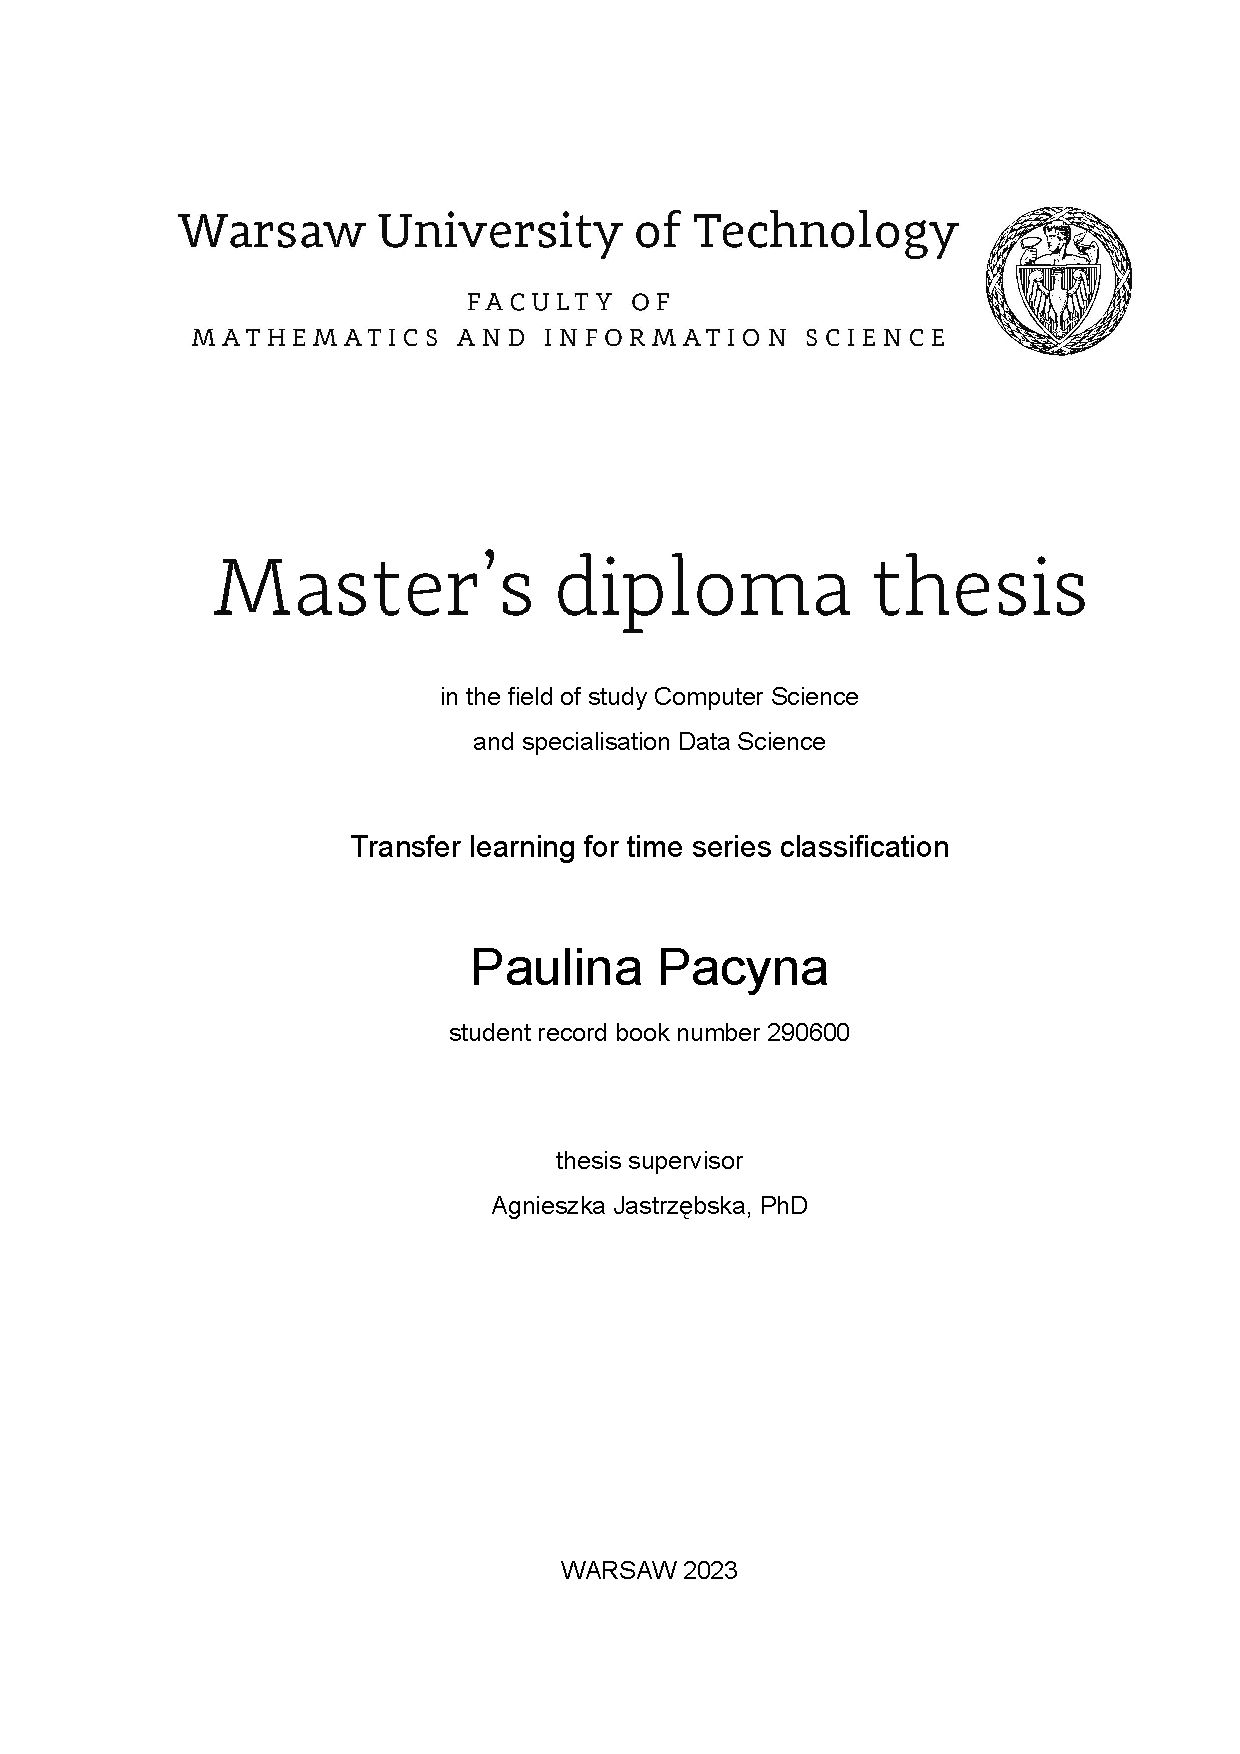
\includepdf[pages=-]{titlepage-en} % THIS INPUTS THE TITLE PAGE

\null\thispagestyle{empty}\newpage

% ------------------ PAGE WITH SIGNATURES --------------------------------

\thispagestyle{empty}\newpage
\null

\vfill

\begin{center}
\begin{tabular}[t]{ccc}
............................................. & \hspace*{100pt} & .............................................\\
supervisor's signature & \hspace*{100pt} & author's signature
\end{tabular}
\end{center}



% ---------------------------- ABSTRACTS -----------------------------

{  \fontsize{12}{14} \selectfont
\begin{abstract}

\begin{center}
\title
\end{center}
The task of classifying time series is an important problem in the field of data mining. Most phenomena that change over time can be described in terms of time series. A time series can describe, for example, the amplitude of a heartbeat sound, stock prices, or hand movement along an axis when serving in tennis. Time series can express different characteristics of the phenomenon. Those characteristics are called \textit{classes}. For example, the heartbeat sound amplitude can represent (belong to) one of two classes: \textit{healthy} and \textit{unhealthy}. Time series classification attempts to learn the distinctive features of a time series and build a model that can distinguish between those classes.

The time series classification problem was initially solved using classical algorithms such as the k-nearest neighbor classifier with distance measures suited for time series, like Dynamic Time Warping. The advantages of using deep learning algorithms in the context of time series classification have recently begun to be recognized. Neural networks can detect shapes that distinguish a class or understand ordered temporal relationships.

Transfer learning is practically used when there is limited data to train. Transfer learning attempts to apply patterns learned from one dataset to improve learning when creating a model for another dataset. A common practice is to prepare a source classifier trained on a large, readily available amount of data for one task and then use this model or parts of it for a detailed task with a smaller amount of data. Models trained using this method often have a shorter training time, faster accuracy increase, and can generalize more easily on the test set.
\newpage
This thesis focuses on proposing, testing, and evaluating multi-source transfer learning for time series classification. We introduce two methods, one of them inspired by the success of ensemble methods in time series classification. Both of those methods apply to most neural network architectures. Both methods were compared to the same network architectures but without transfer learning and proved to improve accuracy and mitigate overfitting.

While transfer learning usually leads to improvements, sometimes \textit{negative transfer} may occur, meaning that the usage of transfer learning is detrimental to the resulting classifier. Negative transfer is especially common when the source domain differs from the target domain or the dataset sizes are small. Given that the datasets present in the time series classification field are usually small, negative transfer may be a threat. This can be mitigated by choosing the source datasets according to the target dataset characteristics.

As the methods proposed in this thesis do not specify which source datasets for the transfer learning are suitable for a given target dataset, we also study the dataset selection method. We compare selecting the source datasets based on a DTW Barycenter Averaging similarity measure to selecting datasets randomly. Datasets chosen in order to minimize the similarity measure lead to improving the target classifier results.

Finally, we study how many source datasets should be used in the transfer learning procedure. We conduct experiments with $3$, $5$, and $8$ source datasets. All those settings result in satisfactory results, and using $5$ source datasets outperforms the two other settings.

\noindent \textbf{Keywords:} time series, classification, transfer learning, deep learning, ensemble, ... % TODO ska supervisor why.. the template also has ", ..." at the end
\end{abstract}
}

\null\thispagestyle{empty}\newpage


{\selectlanguage{polish} \fontsize{12}{14}\selectfont
\begin{abstract}

\begin{center}
\tytul
\end{center}

Zadanie klasyfikacji szeregów czasowych jest ważnym problemem w dziedzinie eksploracji danych. Szeregi czasowe występują za każdym razem, gdy chcemy zmierzyć jakieś zjawisko, które zmienia się w czasie. Szereg czasowy może opisywać np. amplitudę dźwięku bicia serca, ceny akcji czy ruch ręki wzdłuż osi podczas serwu w tenisie. Takie szeregi czasowe mogą wyrażać różne cechy zjawiska. Te cechy nazywane są \textit{klasami}. Na przykład amplituda dźwięku bicia serca może reprezentować (należeć do) jednej z dwóch klas:  \textit{norma}~i~\textit{choroba}. Klasyfikacja szeregów czasowych polega na rozpoznawaniu charakterystycznych cech szeregu czasowego i budowaniu modelu, który potrafi rozróżniać klasy.

Problem klasyfikacji szeregów czasowych był początkowo rozwiązywany za pomocą klasycznych algorytmów, takich jak algorytm k-najbliższych sąsiadów w połączeniu z miarami podobieństwa dla szeregów, ktorym jest dynamiczne marczenie czasu (Dynamic Time Warping). W ostatnim czasie zaczęto dostrzegać zalety stosowania algorytmów głębokiego uczenia w kontekście klasyfikacji szeregów czasowych. Sieci neuronowe są w stanie wykryć kształty wyróżniające daną klasę lub zrozumieć relacje między obserwacjami w czasie.

Metoda transfer learning jest stosowana w przypadku ograniczonej ilości danych do trenowania modelu. Technika transfer learning próbuje zastosować wzorce wyuczone~z~jednego zbioru danych, podczas tworzenia modelu dla innego zbioru danych. Częstą praktyką jest przygotowanie źródłowego klasyfikatora wytrenowanego na dużej, łatwo dostępnej ilości danych dla jednego zadania, a następnie wykorzystanie modelu lub jego części do szczegółowego zadania z mniejszą ilością danych. Modele wytrenowane tą metodą często mają krótszy czas trenowania, szybszy wzrost dokładności i lepsze, ogólniejsze wyniki na zbiorze testowym.

\newpage
Celem pracy dyplomowej jest rozwinięcie badań nad metodą transfer learning w klasyfikacji szeregów czasowych, przez opisanie metod pozwalających na użycie więcej niż jednego zbioru źródłowego. Opisujemy dwie metody, które można stosować do większości sieci neuronowych. W niniejszej pracy została przeprowadzona analiza porównawcza powyższych metod, przez przyrównanie do wyników otrzymanych z wykorzystaniem identycznej co do architektury sieci neuronowej, ale bez metody transfer learningu. Porównujemy obie metody pod kątem czasu trenowania oraz miejsca zajmowanego na dysku.

W metodzie transfer learningu, szczególnie przy klasyfikacji szeregów czasowych, powszechnie występuje efekt negatywnego transferu. Efekt ten ma miejsce, gdy zbiór lub zbiory źródłowe różnią się znacznie od zbioru docelowego. W pracy omawiamy algorytmy doboru zbioru źródłowego do zbioru docelowego na podstawie miar podobieństwa zbiorów, aby zminimalizować efekt negatywnego transferu.

Na koniec analizujemy optymalną liczbę zbiorów źródłowych dla proponowanych metod transfer learningu. Przeprowadzamy eksperymenty z użyciem $3$, $5$ oraz $8$ zbiorów zródłowych.


\noindent \textbf{Słowa kluczowe:} szeregi czasowe, klasyfikacja, transfer learning, ...
\end{abstract}
}


%% --------------------------- DECLARATIONS ------------------------------------
%
%%
%%	IT IS NECESSARY OT ATTACH FILLED-OUT AUTORSHIP DEECLRATION. SCAN (IN PDF FORMAT) NEEDS TO BE PLACED IN scans FOLDER AND IT SHOULD BE CALLED, FOR EXAMPLE, DECLARATION_OF_AUTORSHIP.PDF. IF THE FILENAME OR FILEPATH IS DIFFERENT, THE FILEPATH IN THE NEXT COMMAND HAS TO BE ADJUSTED ACCORDINGLY.
%%
%%	command attacging the declarations of autorship
%%
%\includepdf[pages=-]{scans/declaration-of-autorship}
%\null\thispagestyle{empty}\newpage
%
%% optional declaration
%%
%%	command attaching the declaataration on granting a license
%%
%\includepdf[pages=-]{scans/declaration-on-granting-a-license}
%%
%%	.tex corresponding to the above PDF files are present in the 3. declarations folder
%
\null\thispagestyle{empty}\newpage
% ------------------- TABLE OF CONTENTS ---------------------
% \selectlanguage{english} - for English
\pagenumbering{gobble}
\tableofcontents
\thispagestyle{empty}
\newpage % IF YOU HAVE EVEN QUANTITY OD PAGES OF TOC, THEN REMOVE IT OR ADD \null\newpage FOR DOUBLE BLANK PAGE BEFORE INTRODUCTION
%\null\newpage

% -------------------- THE BODY OF THE THESIS --------------------------------

\null\thispagestyle{empty}\newpage
\pagestyle{fancy}
\pagenumbering{arabic}
\setcounter{page}{11}


\chapter{Introduction}
%\markboth{}{Introduction}
%\addcontentsline{toc}{chapter}{Introduction}
Time series classification was initially approached using classical machine learning algorithms. Bagnall et al.~in  \cite{bake_off} categorize the commonly used algorithms into several categories. The first category is time domain distance-based algorithms. Those algorithms use various distance measures adjusted for the time series domain to capture the similarity between pairs of time series. The distance measure is then combined with a distance-based classifier. A flagship example of an algorithm belonging to this class of algorithms is Dynamic Time Warping distance with the k-Nearest Neighbour classifier. The DTW-1-NN classifier is often used as a benchmark classifier. Another category of classifiers mentioned in \cite{bake_off} are dictionary, shapelet and interval based classifiers. All try to extract distinctive features for the time series class. The dictionary-based classifiers encode the time series into a dictionary of \textit{words} representing the time series. Shapelet-based algorithms focus on subseries of the time series that are discriminatory of class membership. Interval-based algorithms extract features from selected intevals of the time series.

With the rise of the popularity of deep learning algorithms, researchers attempted to replace the former, hand-extracted features and algorithms with deep learning classifiers. Fawaz et al.~reviewed deep learning algorithms applied to the time series classification task \cite{dl_tsc}. The usage of deep learning algorithms enabled the possibility to utilize transfer learning.

Transfer learning is widely used in image recognition and natural language processing. Fawaz et al.~extended their previous findings by a study on the application of transfer learning \cite{dl_tsc}. The authors examine knowledge transferability on 85 datasets from the UCR archive by pre-training a model on one dataset and fine-tuning it on another. The authors examine if the accuracy improved for all pairs of datasets in the UCR archive.

Transfer learning for deep learning is usually done by training the network on a big, diverse dataset and utilizing the first layers of the network when training on another dataset. In image recognition or natural language processing, it is common to pre-train the source network on the ImageNet dataset or Wikipedia dataset, respectively. Such a diverse dataset with labels does not exist for time series. In this thesis, we attempt to create an artificial, diverse dataset from smaller datasets available on the UCR archive. We try to mimic the good properties of a transfer learning source dataset by preprocessing, upsampling, and augmenting the dataset. We also study if transfer learning on a diverse dataset helps to generalize new training data and improve the training process on the target dataset. Similarly, as in \cite{imagnet}, we experiment to find which features of the source dataset (classes diversity, dataset size, augmentation, preprocessing) are fundamental for the transfer learning process.

%TODO We wstępie brakuje konkretnego, szczegółowego wymienienia zakresu (celów pracy). Proszę dodać odpowiedni paragraf nie martwiąc się tym, że “zdradzi” Pani częściowo wyniki końcowe.
%
%Kończący paragraf opisuje strukturę pracy. czyli “ W rozdziale 2 przedstawiono …”
%What is the thesis about? What is the content of it? What is the Author's contribution to it?
%\par
%WARNING!  In a diploma thesis which is a team project: Description of the work division in the team, including the scope of each co-author’s contribution to the practical part (Team Programming Project) and the descriptive part of the diploma thesis.
%\par
\chapter{Related works}
In this chapter, we describe several algorithms used in time series classification, focusing on deep learning algorithms. We refer to literature and papers in the domain of time series classification and transfer learning. We also describe the most popular archive of time series datasets, the UCR archive.


\section{Time series classification}
A time series is an ordered collection of observations indexed by time.
$$X = (x_t)_{t\in T} = (x_1, ... , x_T),\ x_t\in \real$$
The time index $T$ can represent any collection with the natural order. We assume that indices are spaced evenly in the set $T$. The realization or observation $x_t$ in the times series is a numerical value describing the phenomena we observe, for example, the amplitude of a sound, stock price, or y-coordinate. Time series classification is a problem of finding the optimal mapping between a set of time series and corresponding classes.



\subsection{Multi Layer Perceptron}\label{mlp_section_related}
The Multi Layer Perceptron (MLP) is the first artificial neural network architecture proposed in \cite{dl_tsc} and can be used for time series classification tasks.
%A MLP network can be formally defined as a function depending on a set \textit{weights} $\theta_i$.
%$$MLP(X; \theta_1,\dots , \theta_M, \beta_1,\dots , \beta_M) = f_M( \beta_M +  \theta_M \cdot (f_{M-1}( \beta_{M-1} +  \theta_{M-1} \cdot (\dots f_1( \beta_1 +  \theta_1 \cdot X)))))$$
Formally, the MLP network can be defined as a composition of functions (called \textit{dense layers} or \textit{layers}). The network returns a vector that usually represents the probability distribution over the set of classes.
$$MLP(X; \theta_1,\dots , \theta_M, \beta_1,\dots , \beta_M) = L_M(\dots L_2(L_1(X;\theta_1, \beta_1);\theta_2, \beta_2);\theta_M, \beta_M)$$
Each layer $L_i: \real^M \rightarrow \real^N$ is a function that depends on the parameters $\theta \in r^{M\times N}, \beta \in \real^N$
$$L_i(X ; \theta_i, \beta_i) = f_i(X \theta_i  + \beta_i)$$
The function $f_i: \real^N \rightarrow \real^N$ is an arbitrarily chosen non-linear function. The number of layers and dimension of weights in hidden layers is also arbitrary. The weights in the first and last layer have to match the dimensionality of input data (e.g.~the length of the time series) and the number of classes. The output of the last layer is interpreted as a probability distribution over the set of classes.

The disadvantage of using Multi Layer Perceptrons for time series classification is that the input size is fixed. All time series in the training data must have the same length. In transfer learning, this means that if we want to reuse the source network (or a set of first layers from the network), the time series in the target dataset must have the same length as in the source dataset.

The MLP architecture fails at understanding the temporal dependencies \cite{dl_tsc}. Each input value in the time series is treated separately because it is multiplied by a separate row in the weight matrix (see Figure \ref{fig:mlp_multiplication} for an illustration).
\begin{figure}
\centering
\label{fig:mlp_multiplication}
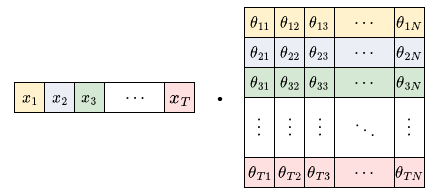
\includegraphics[height=4cm]{imgs/MLP_multiplication_v2.png}
\caption{The multi layer perceptron architecture treats each entry in the input time series separately.}
\end{figure}
\subsection{Convolutional Neural Networks}
Convolutional Neural Networks are widely used in image recognition. A convolution applied for a time series can be interpreted as sliding a filter over the time series. A convolutional layer is a set of functions called convolutions or filters. The filter is applied at a given point, using the values surrounding the point.

To define the convolution operation, let's assume the input is a matrix $X \in \real^{(N_1, \dots, N_K)}$. In the case of images, the number of dimensions $K$ is often equal to $3$ (height, width, channels), for univariate time series we can assume just one dimension, and for multivariate time series we need two dimensions - (feature, time).
The filter consists of a matrix of weights $M \in \real^{(P_1, \dots, P_K)}$.
Usually, $P_l$ are odd numbers, so that we can index the matrix with symmetrical numbers: $ (\frac{-P_l+1}{2},  \frac{-P_l+3}{2}, \dots, 0, \dots, \frac{P_l-1}{2})$. The $0$ index marks the center of the matrix.
%TODO - powolac sie czemu nieparzyscie

Finally the convolution $*$ is defined as follows:
$$(X*M)_{i_1, \dots, i_K} = \sum_{l_1=\frac{-P_1+1}{2}}^{\frac{P_1-1}{2}} \cdots \sum_{l_K=\frac{-P_K+1}{2}}^{\frac{P_K-1}{2}} M_{l_1, \dots, l_K} X_{i_1 + l_1, \dots, i_K + l_K}$$

The result of the convolution is passed elementwise to a nonlinear function. The nonlinear function, together with the convolution operation, is called a filter.
In the case of univariate time series, the first layer of the convolutional neural network is one-dimensional. The output of the first layer has dimensions (length of time series - the length of the filter + 1, number of filters). Below we define the value of the output for filter $i$
$$ y_{t, i} = f_i([\theta_{\frac{-M+1}{2}}^i, \dots , \theta_{\frac{M-1}{2}}^i] \cdot [X_{t+\frac{-M+1}{2}}, \dots, X_{t+\frac{M-1}{2}}]),$$
where $\cdot$ is a dot product and $t \in T$ is the time index.
In Figures \ref{fig:convolution_output_growth} and \ref{fig:convolution_output_hill} we show the results of applying two different filters to a time series.
% TODO ctrl f czy wszystkie Figures maja \ref

\FloatBarrier

\begin{figure}[h!t]
\centering
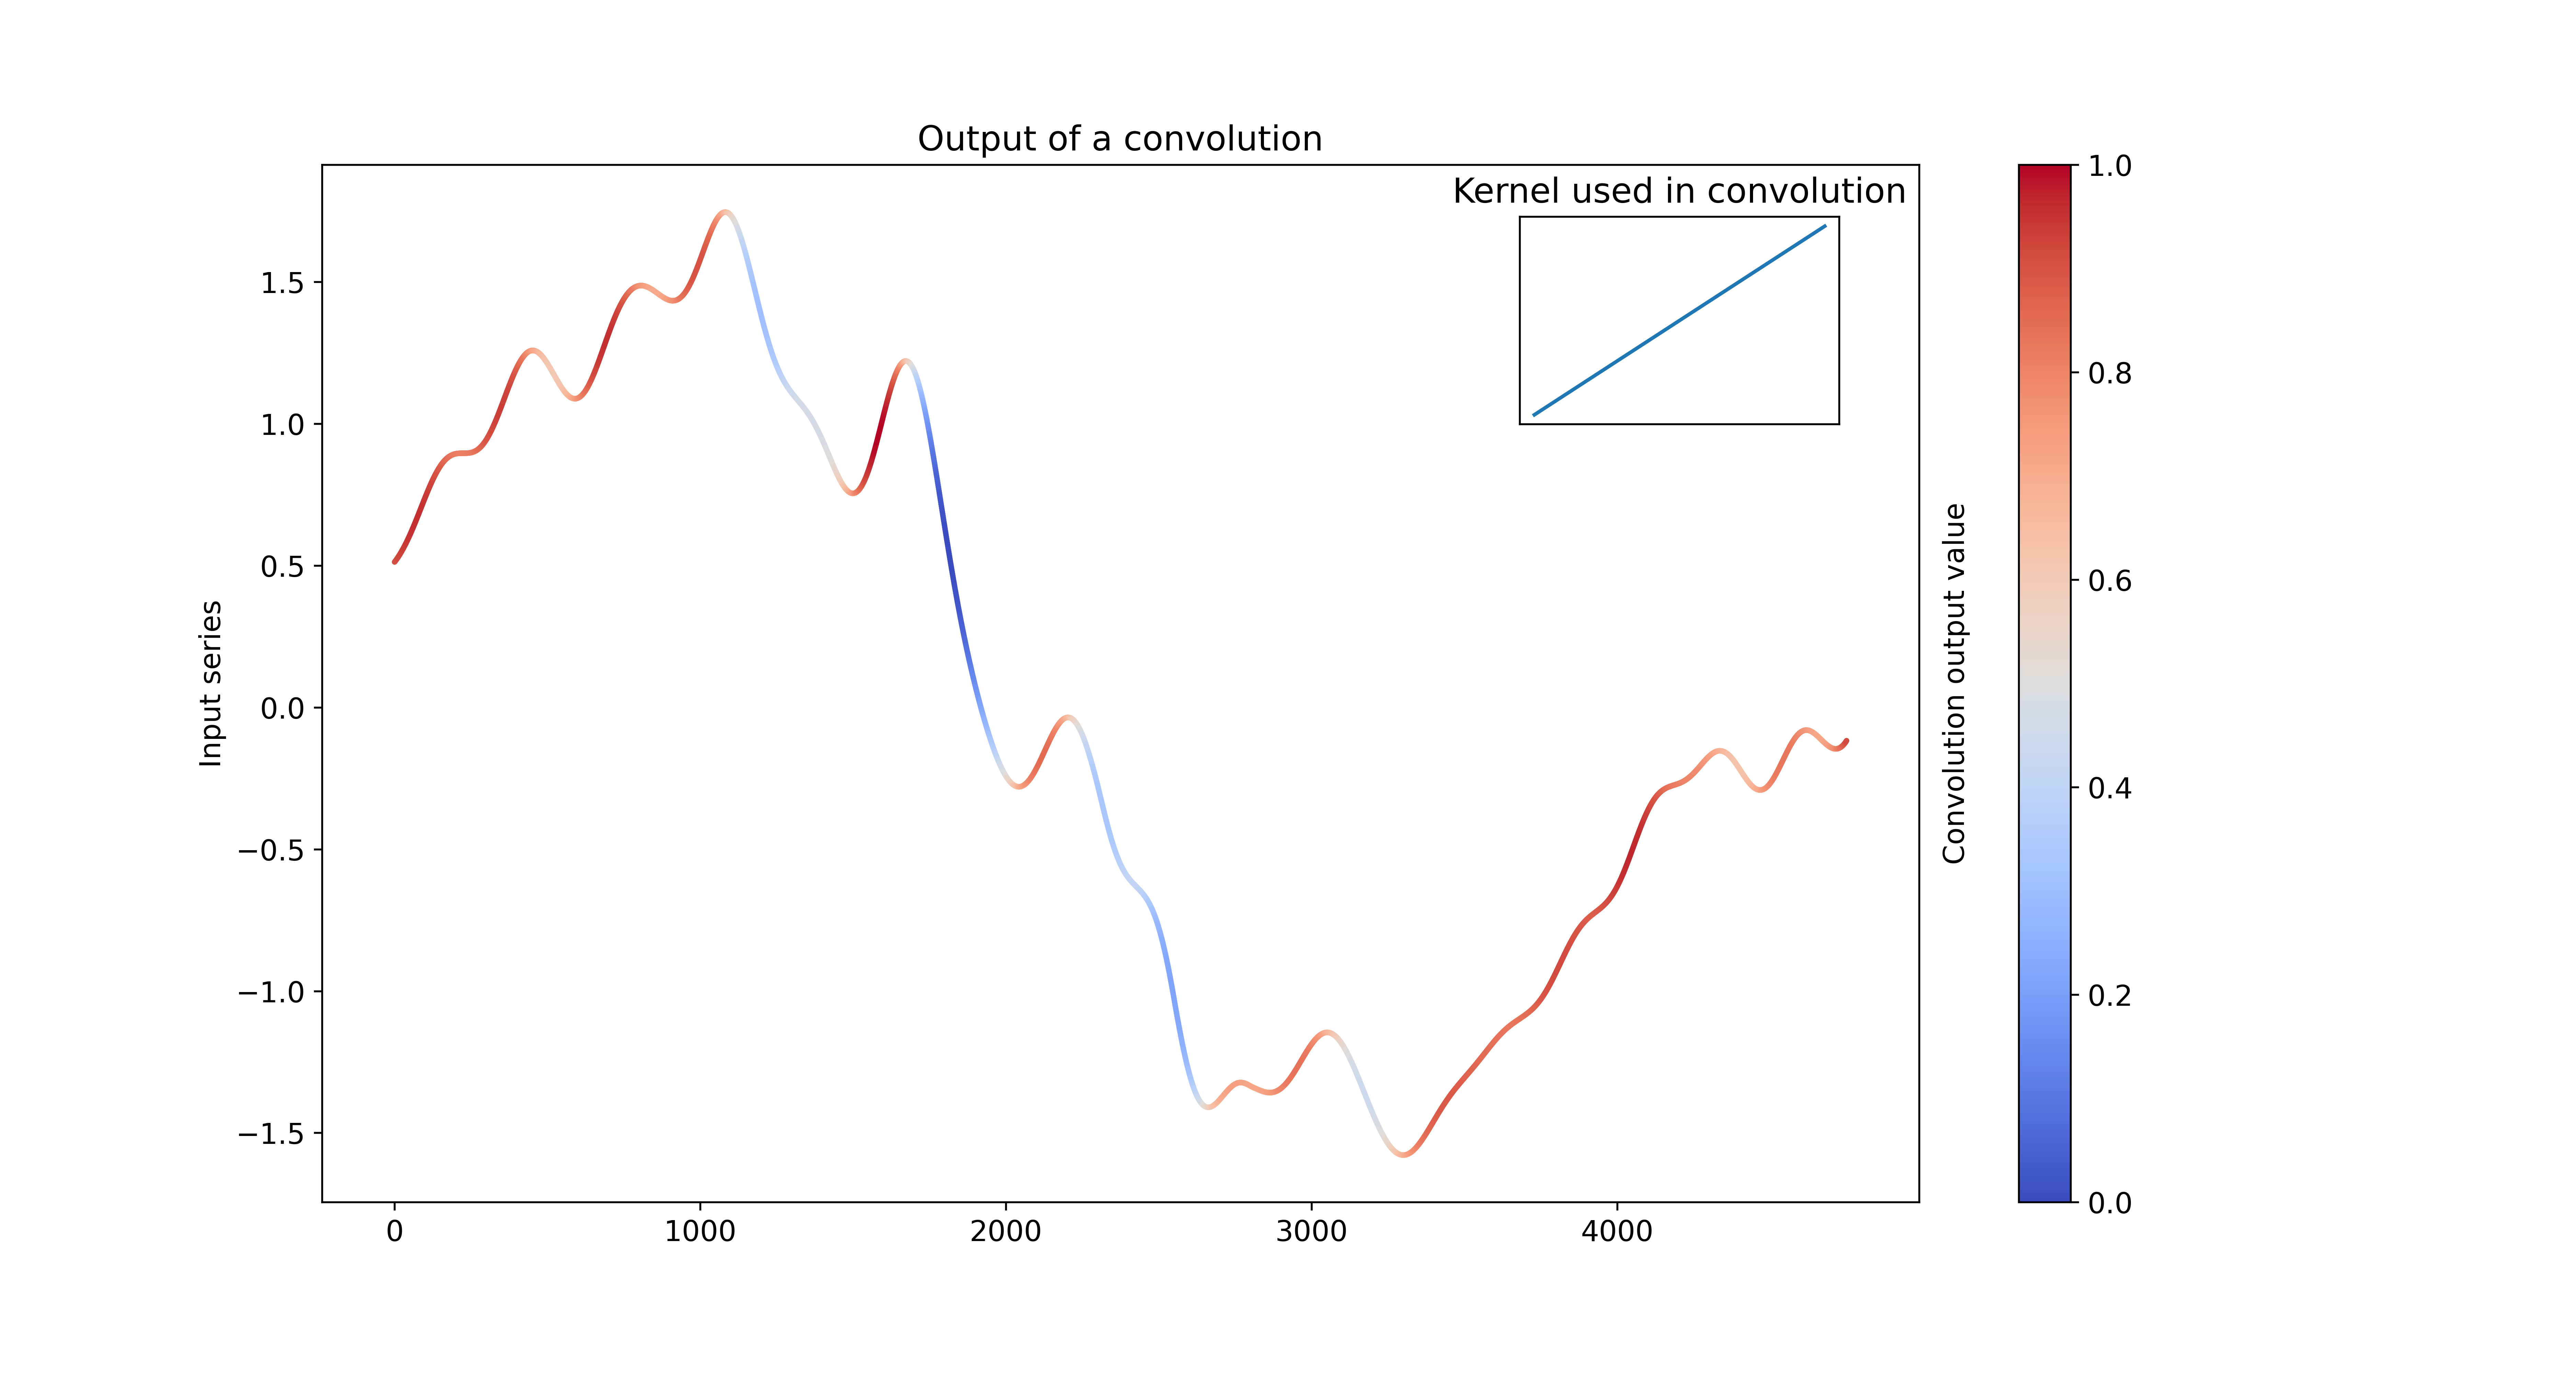
\includegraphics[width=17cm]{imgs/convolution_output_growth.png}
\caption{Result of applying a ``slope'' detecting filter to time series. Red regions indicate a higher value in the time series returned by the output convolution.}
\label{fig:convolution_output_growth}
\end{figure}
\FloatBarrier
\begin{figure}[h!]
\centering
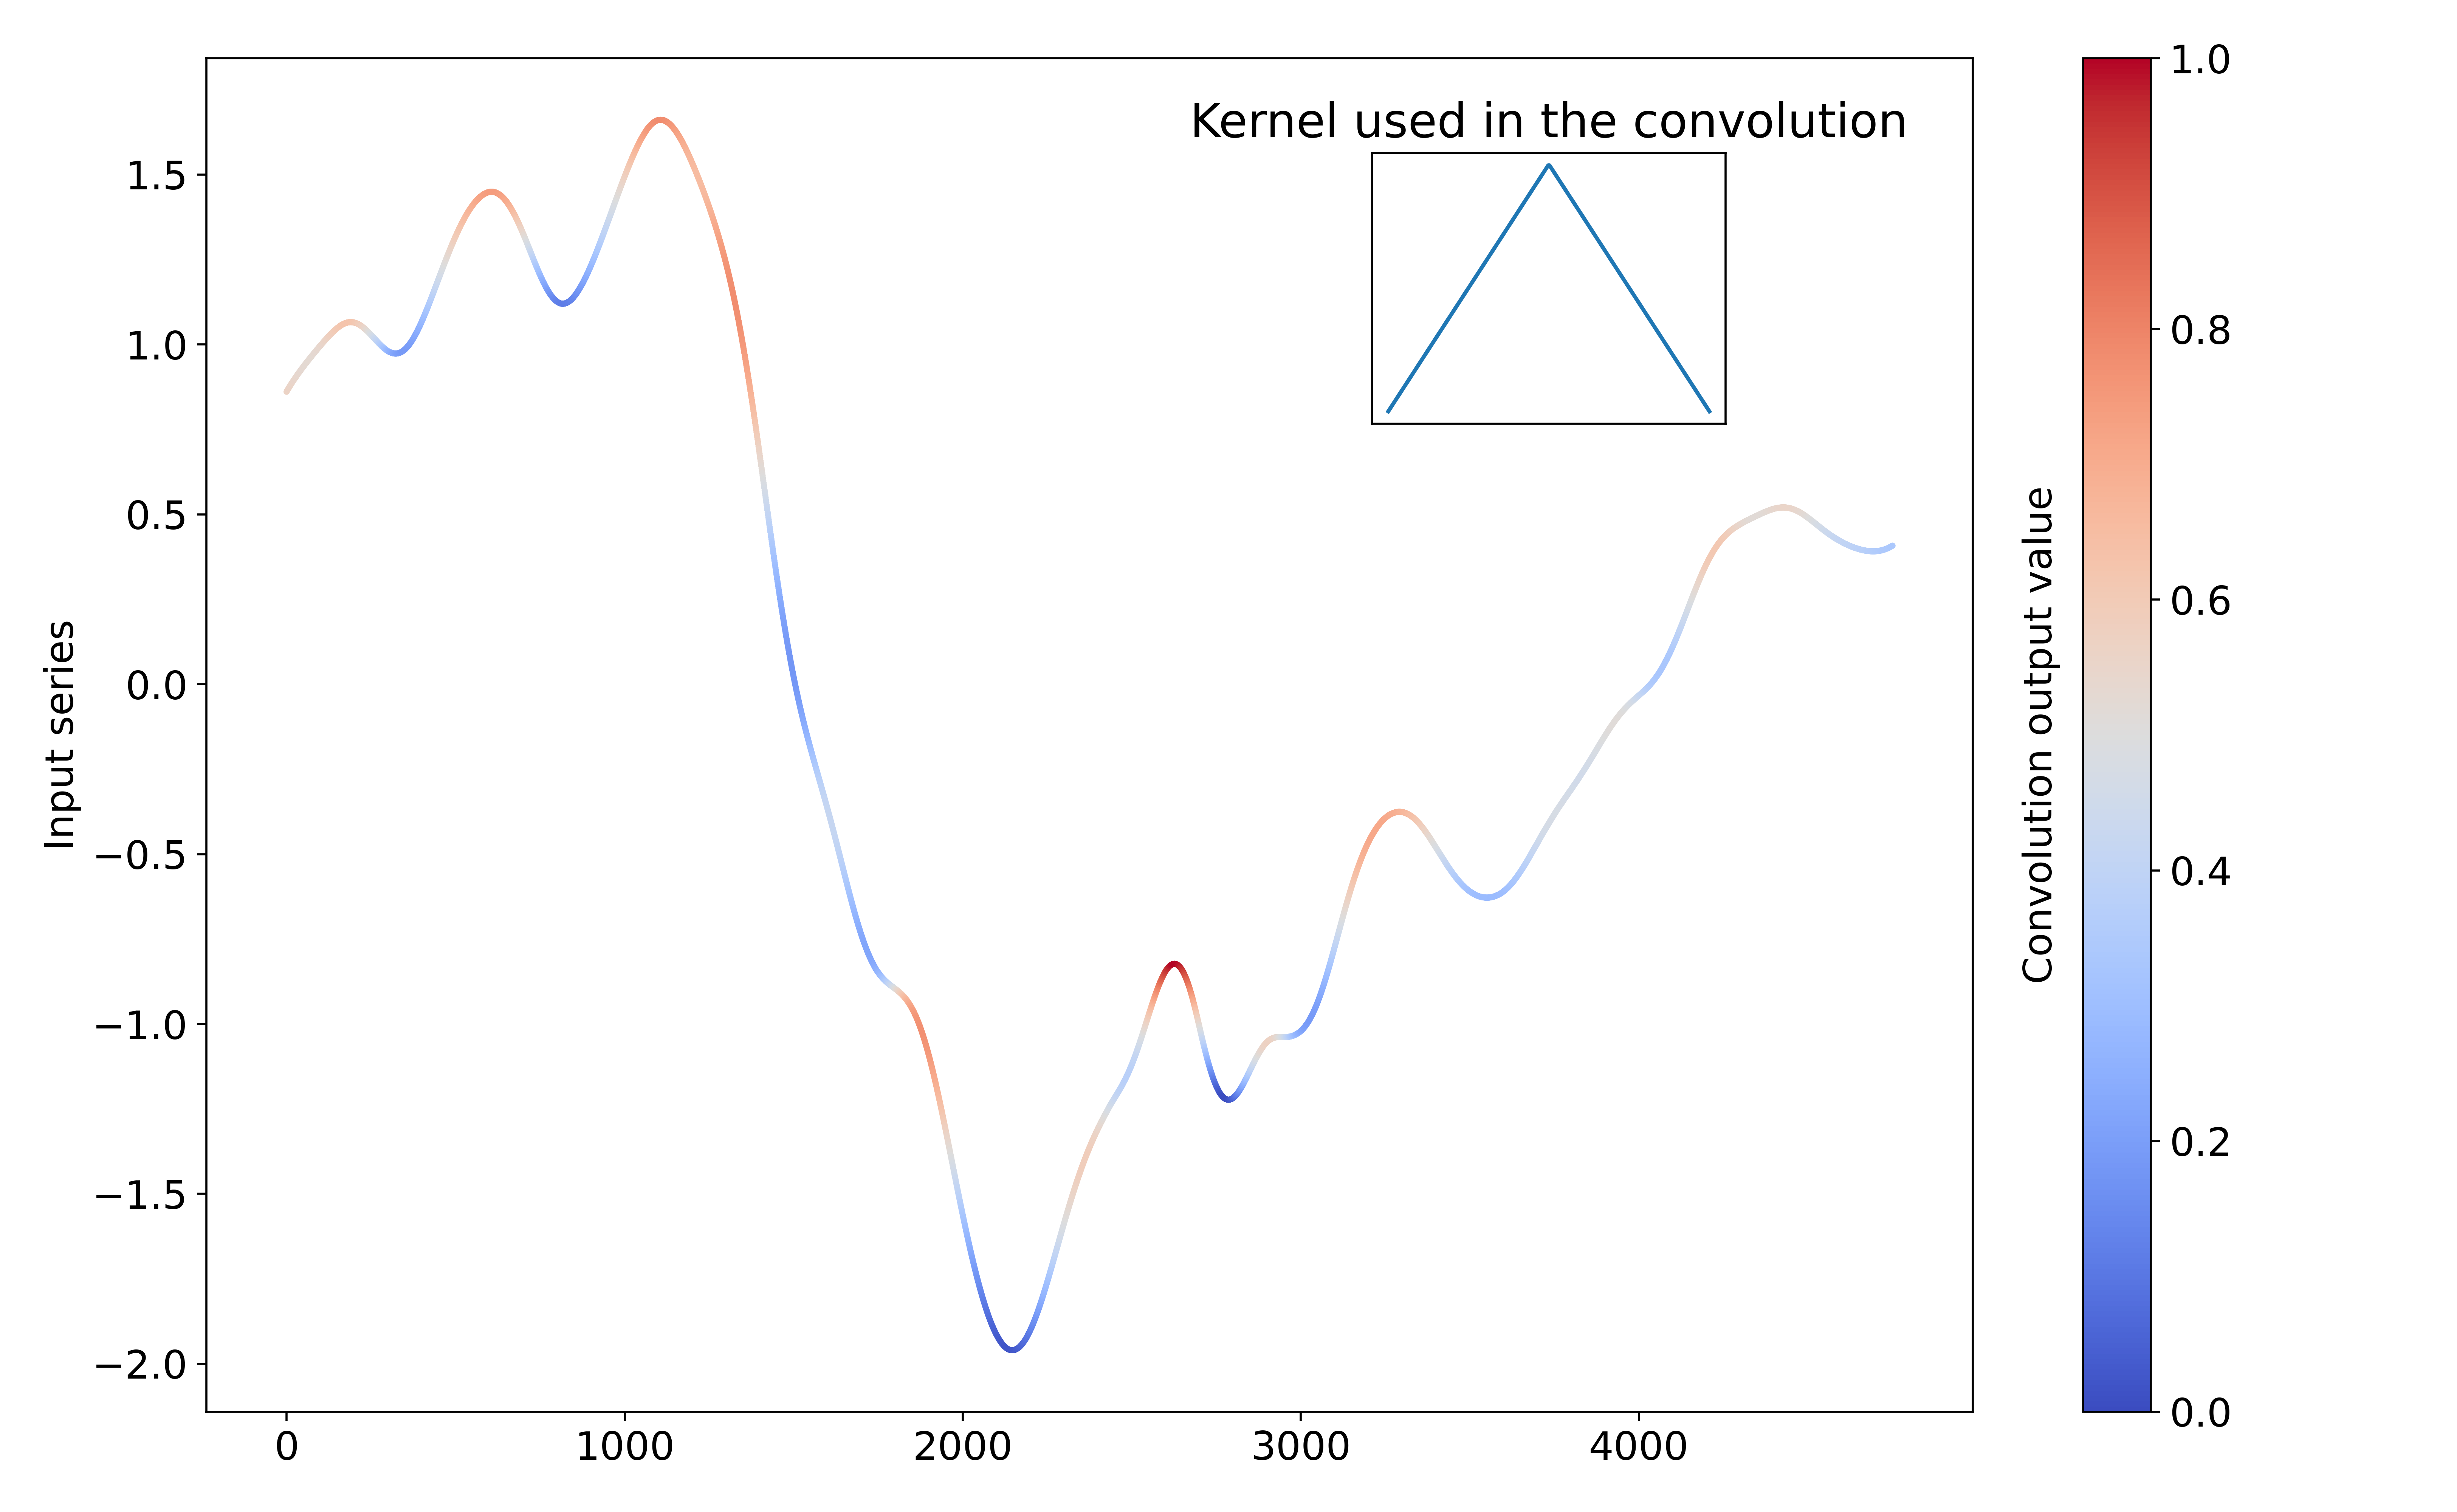
\includegraphics[width=17cm]{imgs/convolution_output_hills.png}
\caption{Result of applying a ``peak'' detecting filter to a time series. Red regions indicate a higher value in the time series returned by the output convolution.}
\label{fig:convolution_output_hill}
\end{figure}

\FloatBarrier

The weights $\theta^i$ are different for each filter.
The same filter is applied over the whole length of the time series. This is called \textit{weight sharing}, enabling the network to learn patterns regardless of the position in the time series.

The architecture of the convolutional layer is not dependent on the input data size. Regardless of the size of the input data, the number of filters and size of filters remain the same, and only the output sizes depend on the input size. Therefore, if the convolutional layer is  succeeded by layers with the same property, like other convolutional layers or Global Pooling with Dense Layer (see Section \ref{FCN}), the whole network may be invariant to the input sizes \cite{dl_tsc}. Such networks may be interesting in transfer learning, as the sizes of time series in the source and target tasks do not have to match.

\subsection{Fully Convolutional Networks}\label{FCN}
Fully Convolutional Networks are convolutional networks used in time series classification. A sample architecture of a Fully Convolutional Network proposed is in \cite{dl_tsc}. The first layers in the network are 3 blocks of convolutional layers with ReLU activation function followed by batch normalization layers. The output of the last block is passed to a global pooling layer. The global pooling layer averages the output through the time axis, resulting in a vector of length equal to the number of feature maps in the last convolutional layer. The averaged vector is passed to a block of 2 fully connected layers. Figure \ref{fig:FCN_img} shows a visualization of the network.



\FloatBarrier

\begin{figure}[h!]
\centering
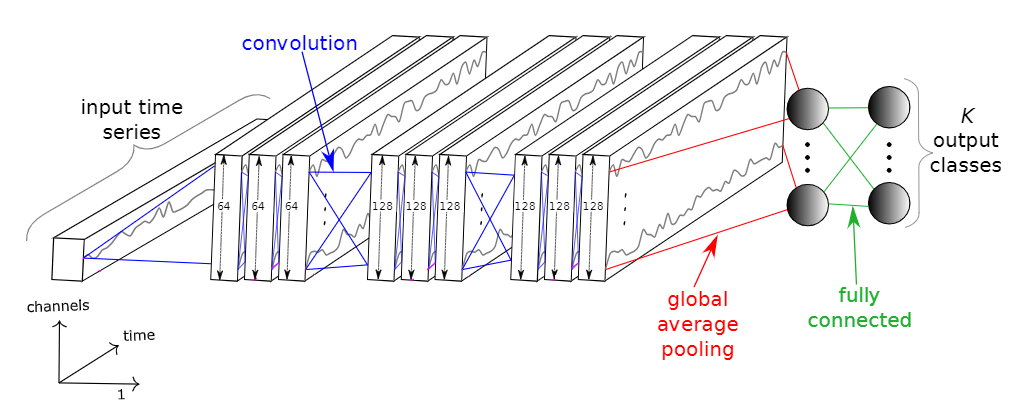
\includegraphics[width=15.5cm]{imgs/fcn.png}
\caption{Architecture of a Fully Convolutional Network. Source: \cite{dl_tsc}}
\label{fig:FCN_img}
\end{figure}

\FloatBarrier

Because the architecture of convolutional layers does not depend on the size of input data and the convolutional layers are followed by pooling over the time axis, the whole network is capable of processing data of variable lengths.
\subsection{Residual Network}
The Residual Network was first proposed by Zhiguang, Weizhong et al.~in \cite{residual}. The Residual Network is suitable for relatively deep architectures compared to other neural networks used for time series classification.

A residual connection addresses the vanishing gradient problem occurring in networks composed of many layers \cite{residual}. The vanishing gradient problem occurs in the backpropagation process. When the gradient passes from the last layer to the first, it may decrease toward zero. This causes the first layers of the network to learn slowly. The residual connection between layers passes the input directly from one layer to another, skipping a few layers. This way, if the network is struggling with a vanishing gradient, this shortcut connection may help the network to converge.

The architecture of the Residual Network is conceptually similar to the FCN network. Instead of three convolutional layers, the Residual Network begins with three blocks of convolutional layers, connected with residual connections. Each block consists of three convolutional layers. The three blocks, which consist of nine convolutional layers and three residual connections in total, are followed by a Global Average Pooling layer and a Dense layer. The networks' diagram is shown below (Figure \ref{fig:Resnet_img}).


\FloatBarrier

\begin{figure}[h!]
\centering
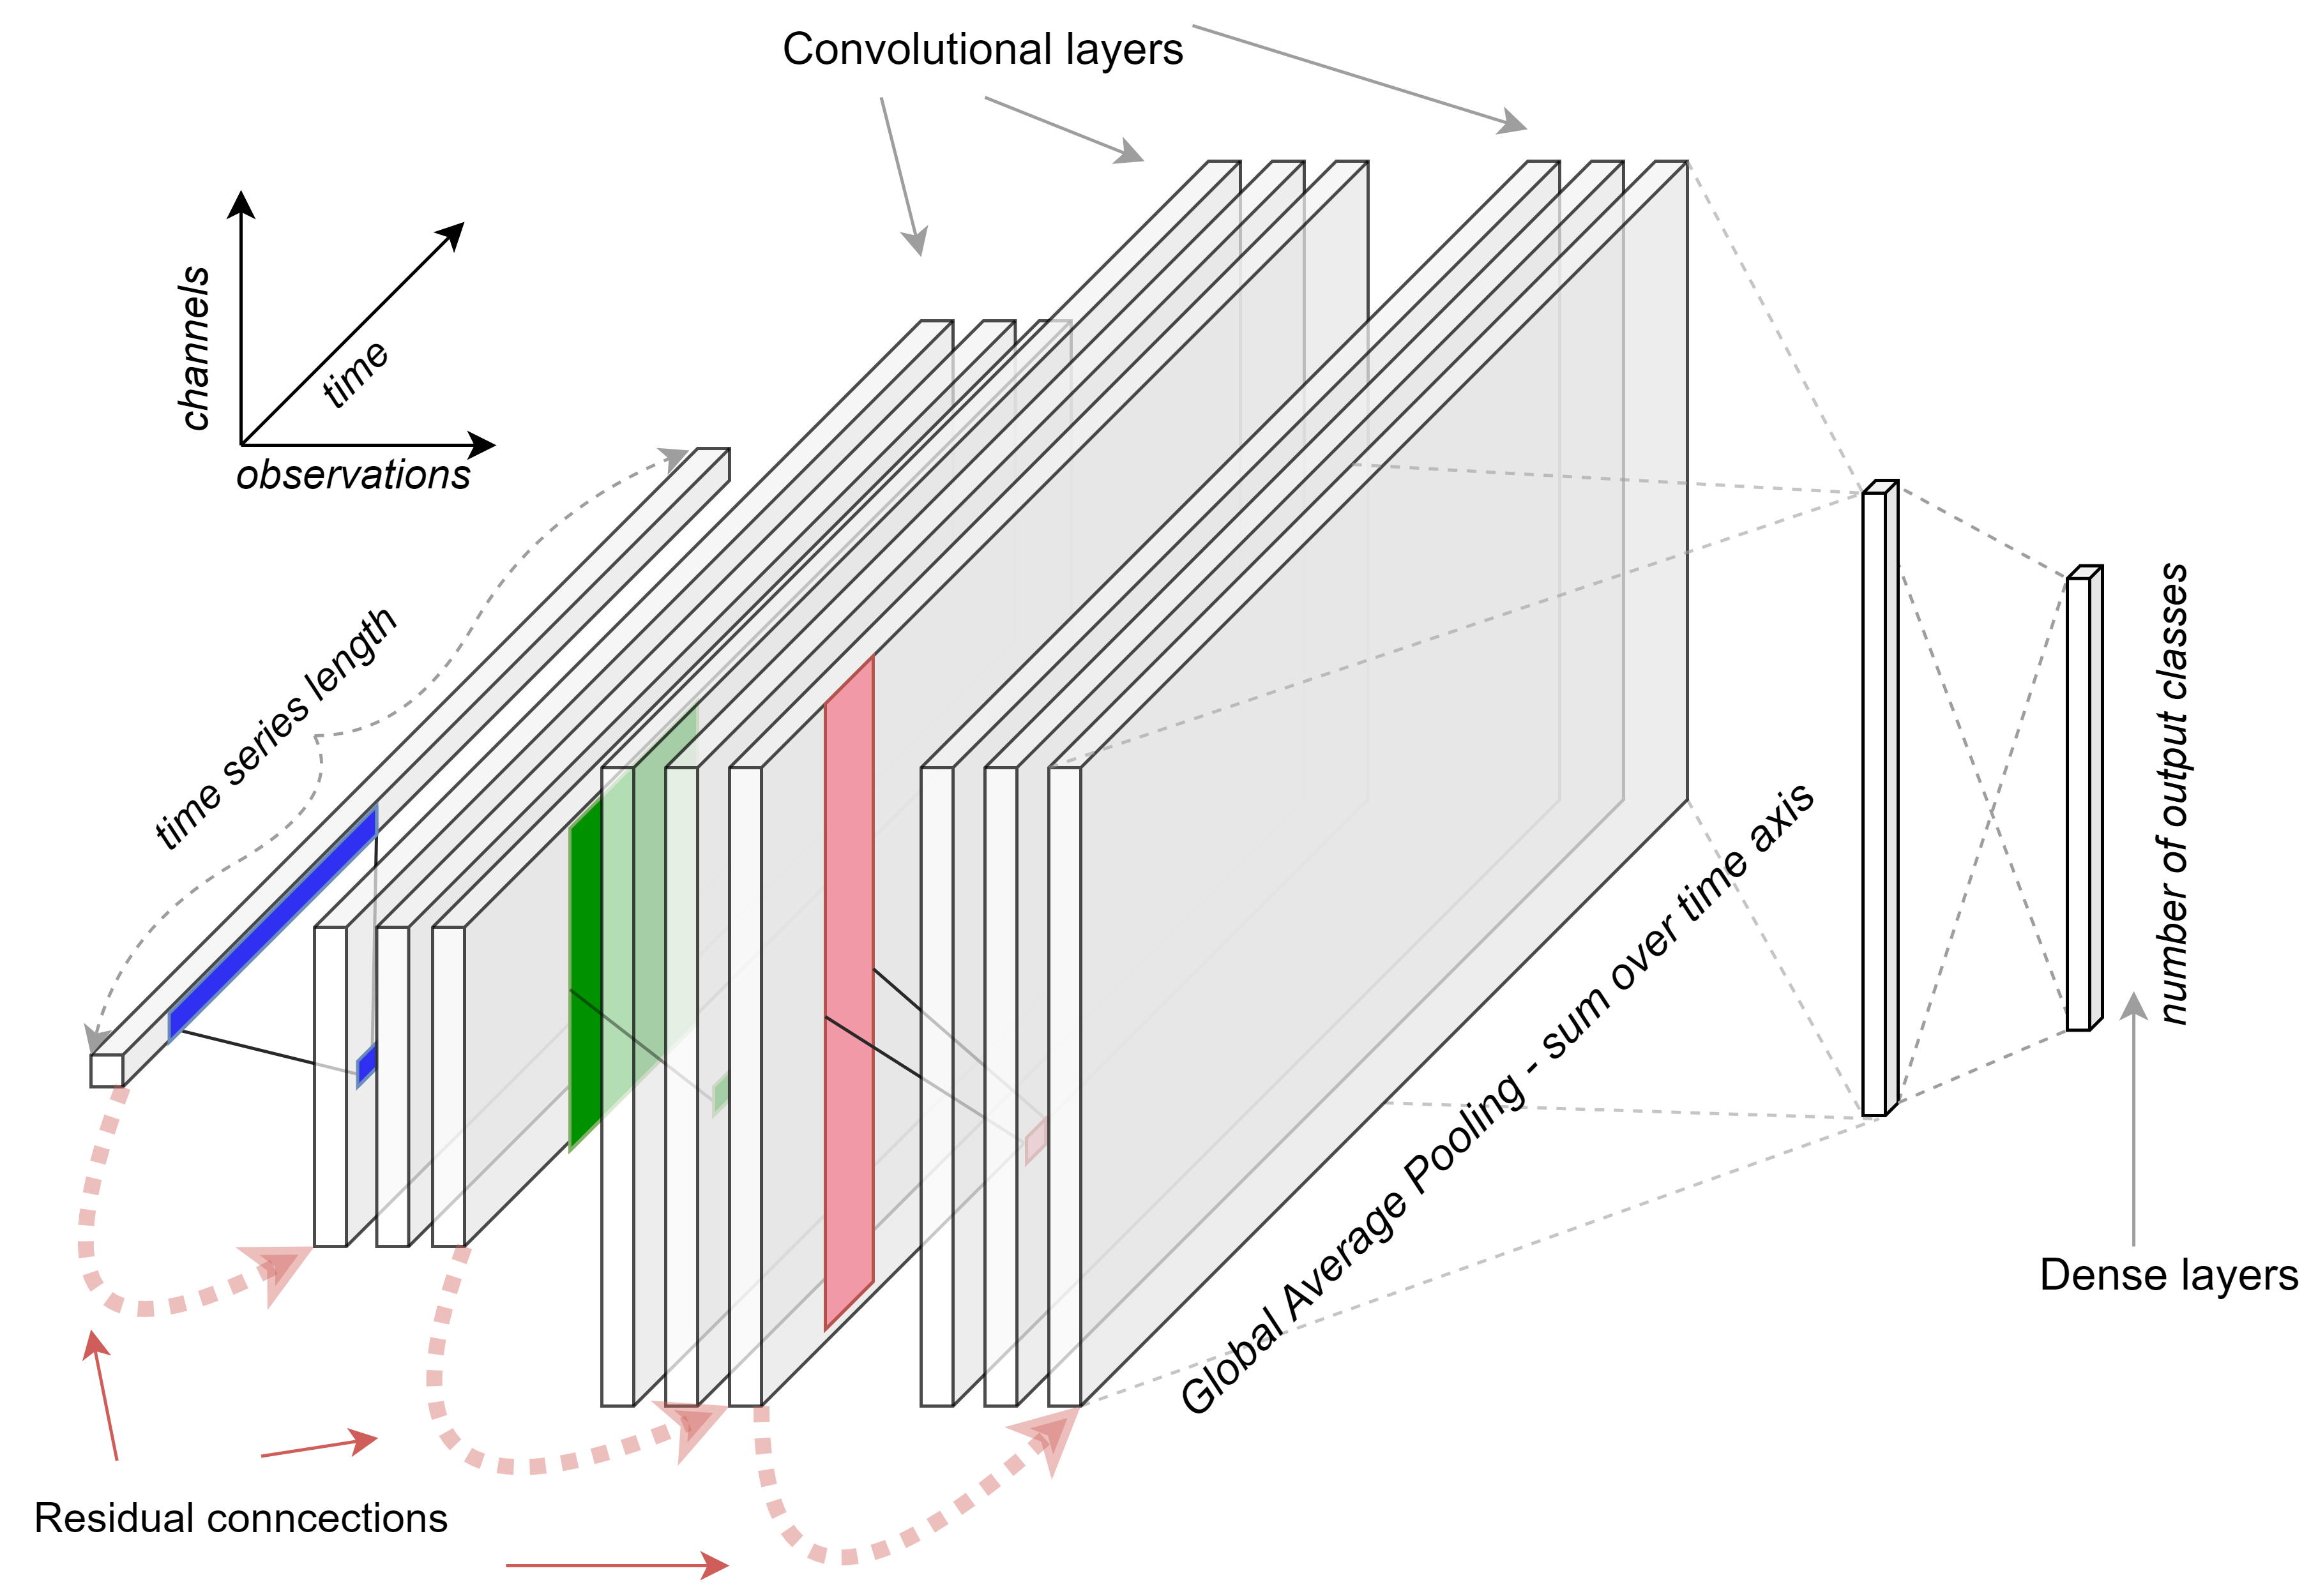
\includegraphics[width=15.5cm]{imgs/resnet.png}
\caption{Architecture of a Residual Network. Source: \cite{dl_tsc}}
\label{fig:Resnet_img}
\end{figure}

\FloatBarrier

\subsection{Encoder Network}
 The Encoder Network is a deep convolutional network proposed by \cite{encoder}. The first layers of the network are similar to the FCN architecture. The network consists of three convolutional layers followed by an attention layer instead of the Global Average Pooling layer. Another novelty introduced in this network compared with the FCN architecture is adding a DropOut layer and replacing the ReLU activation function with PReLU (Parametrized ReLU), thus adding another parameter to the network. The network ends with a Dense layer predicting the distribution over the classes. The architecture is shown below (Figure \ref{fig:encoder_img}).

\FloatBarrier

\begin{figure}[h!]
\centering
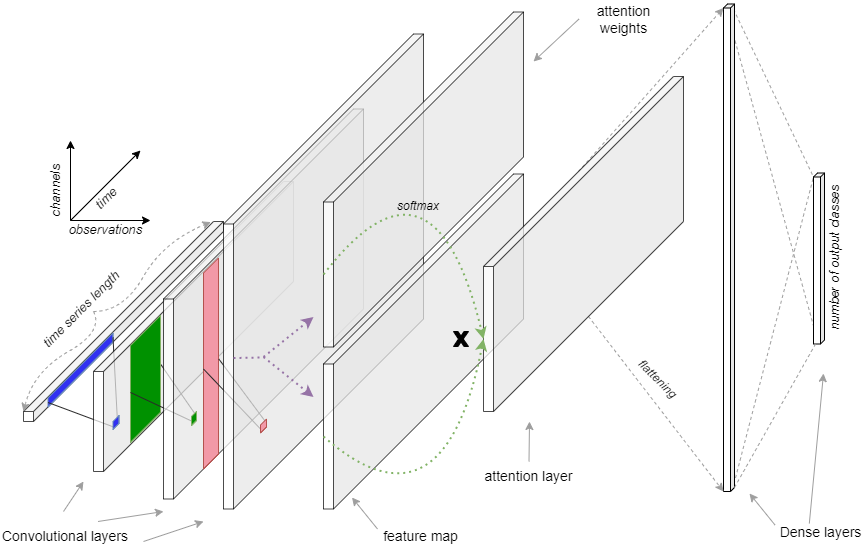
\includegraphics[width=15.5cm]{imgs/encoder.png}
\caption{Architecture of an Encoder Network. Source: \cite{dl_tsc}}
\label{fig:encoder_img}
\end{figure}

\FloatBarrier

The attention layer, first proposed in \cite{attention}, assigns weights to each input element representing the importance of the prediction. The weights representing the attention are normalized using the softmax function and then applied to the input data. The weights  are learned by the network. The outputs of the attention layer can be interpreted as a universal representation of the input time series that can adapt to and represent unseen data \cite{encoder}.

As opposed to the FCN network architecture, the Encoder network is not invariant to the input size. The Dense layer parameters depend on the output size of the attention layer and implicitly on the output size of convolutional layers.  Similarly, as in the former architecture, the convolutional layers enable weight sharing, thus learning shapelets independently of their position in the time series.


\section{The UCR archive}
The URC (University of California, Riverside) archive is a time series classification archive introduced in 2002 by Dau, Keogh et al.~\cite{UCR_archive}. At the moment of writing this thesis, it consists of 140 univariate time series datasets. The time series describes various phenomena, like readings from a device or sensor, motion recordings, or food spectrographs. The time series types are summarized below (Table \ref{table:ucr_summary}). We also show several time series samples from different datasets below (Figure \ref{fig:UCR_samples}).
\begin{table}[!h]
\centering
\tabcolsep=0.11cm
\scalebox {0.9}{
\begin{tabular}{@{}|l|l|@{}}
%\begin{singlespace}
% TODO sprawdzic dlaczego usunęłam HRM
% TODO dodać POWER do DEVICE
% TODO  add SharePriceIncrease


\toprule
\textbf{Dataset type (source)}       & \textbf{Number of datasets} \\ \midrule
Audio                                & 10
\\ \midrule
Device                               & 10                           \\ \midrule
ECG (Electrocardiogram)              & 7 \\ \midrule
EOG (Electrooculography)             & 2                           \\ \midrule
EPG (Electrical penetration   graph) & 2                           \\ \midrule
Hemodynamics                         & 3                           \\ \midrule
Image                                & 33                          \\ \midrule
Motion                               & 28 \\ \midrule
Sensor                               & 22                          \\ \midrule
Simulated                            & 9                           \\ \midrule
Spectro                              & 12       \\ \midrule
Traffic                              & 2                           \\ \bottomrule
%\end{singlespace}
\end{tabular}
}
\caption{Summary of types of datasets in the UCR archive.}
\label{table:ucr_summary}
\end{table}
\FloatBarrier

\begin{figure}[h!]
\centering
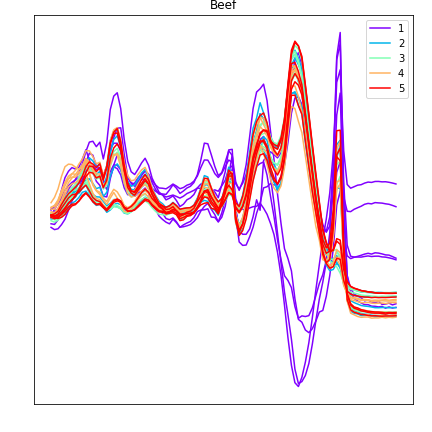
\includegraphics[height=7cm]{imgs/UCR_Beef.png}
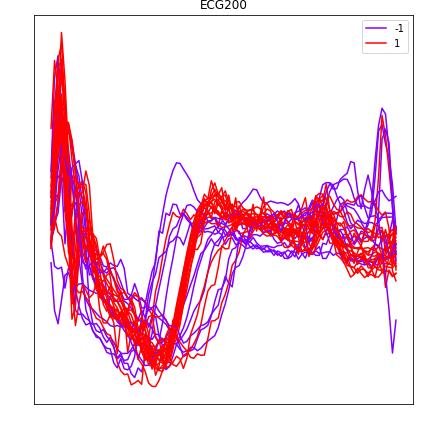
\includegraphics[height=7cm]{imgs/UCR_ECG200.png}
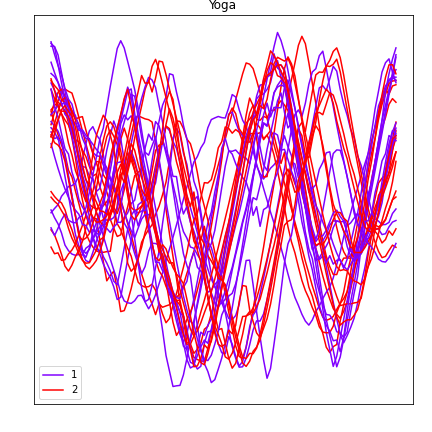
\includegraphics[height=7cm]{imgs/UCR_Yoga.png}
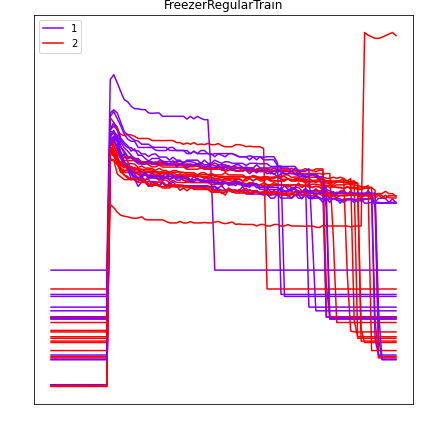
\includegraphics[height=7cm]{imgs/UCR_FreezerRegularTrain.png}
\caption{Example time series from the UCR archive. The images belong to the following categories: Food, ECG, Image, Device.}
\label{fig:UCR_samples}
\end{figure}
All datasets together contain 1122 unique labels. Most datasets differentiate between two labels and have several dozen rows per class. The series length varies from 8 to almost 300 thousand. Below we show four histograms summarizing the number of classes per dataset, the lengths of the series, and the number of observations per class and per dataset. (Figure \ref{fig:histograms})
\begin{figure}[h!]
\centering
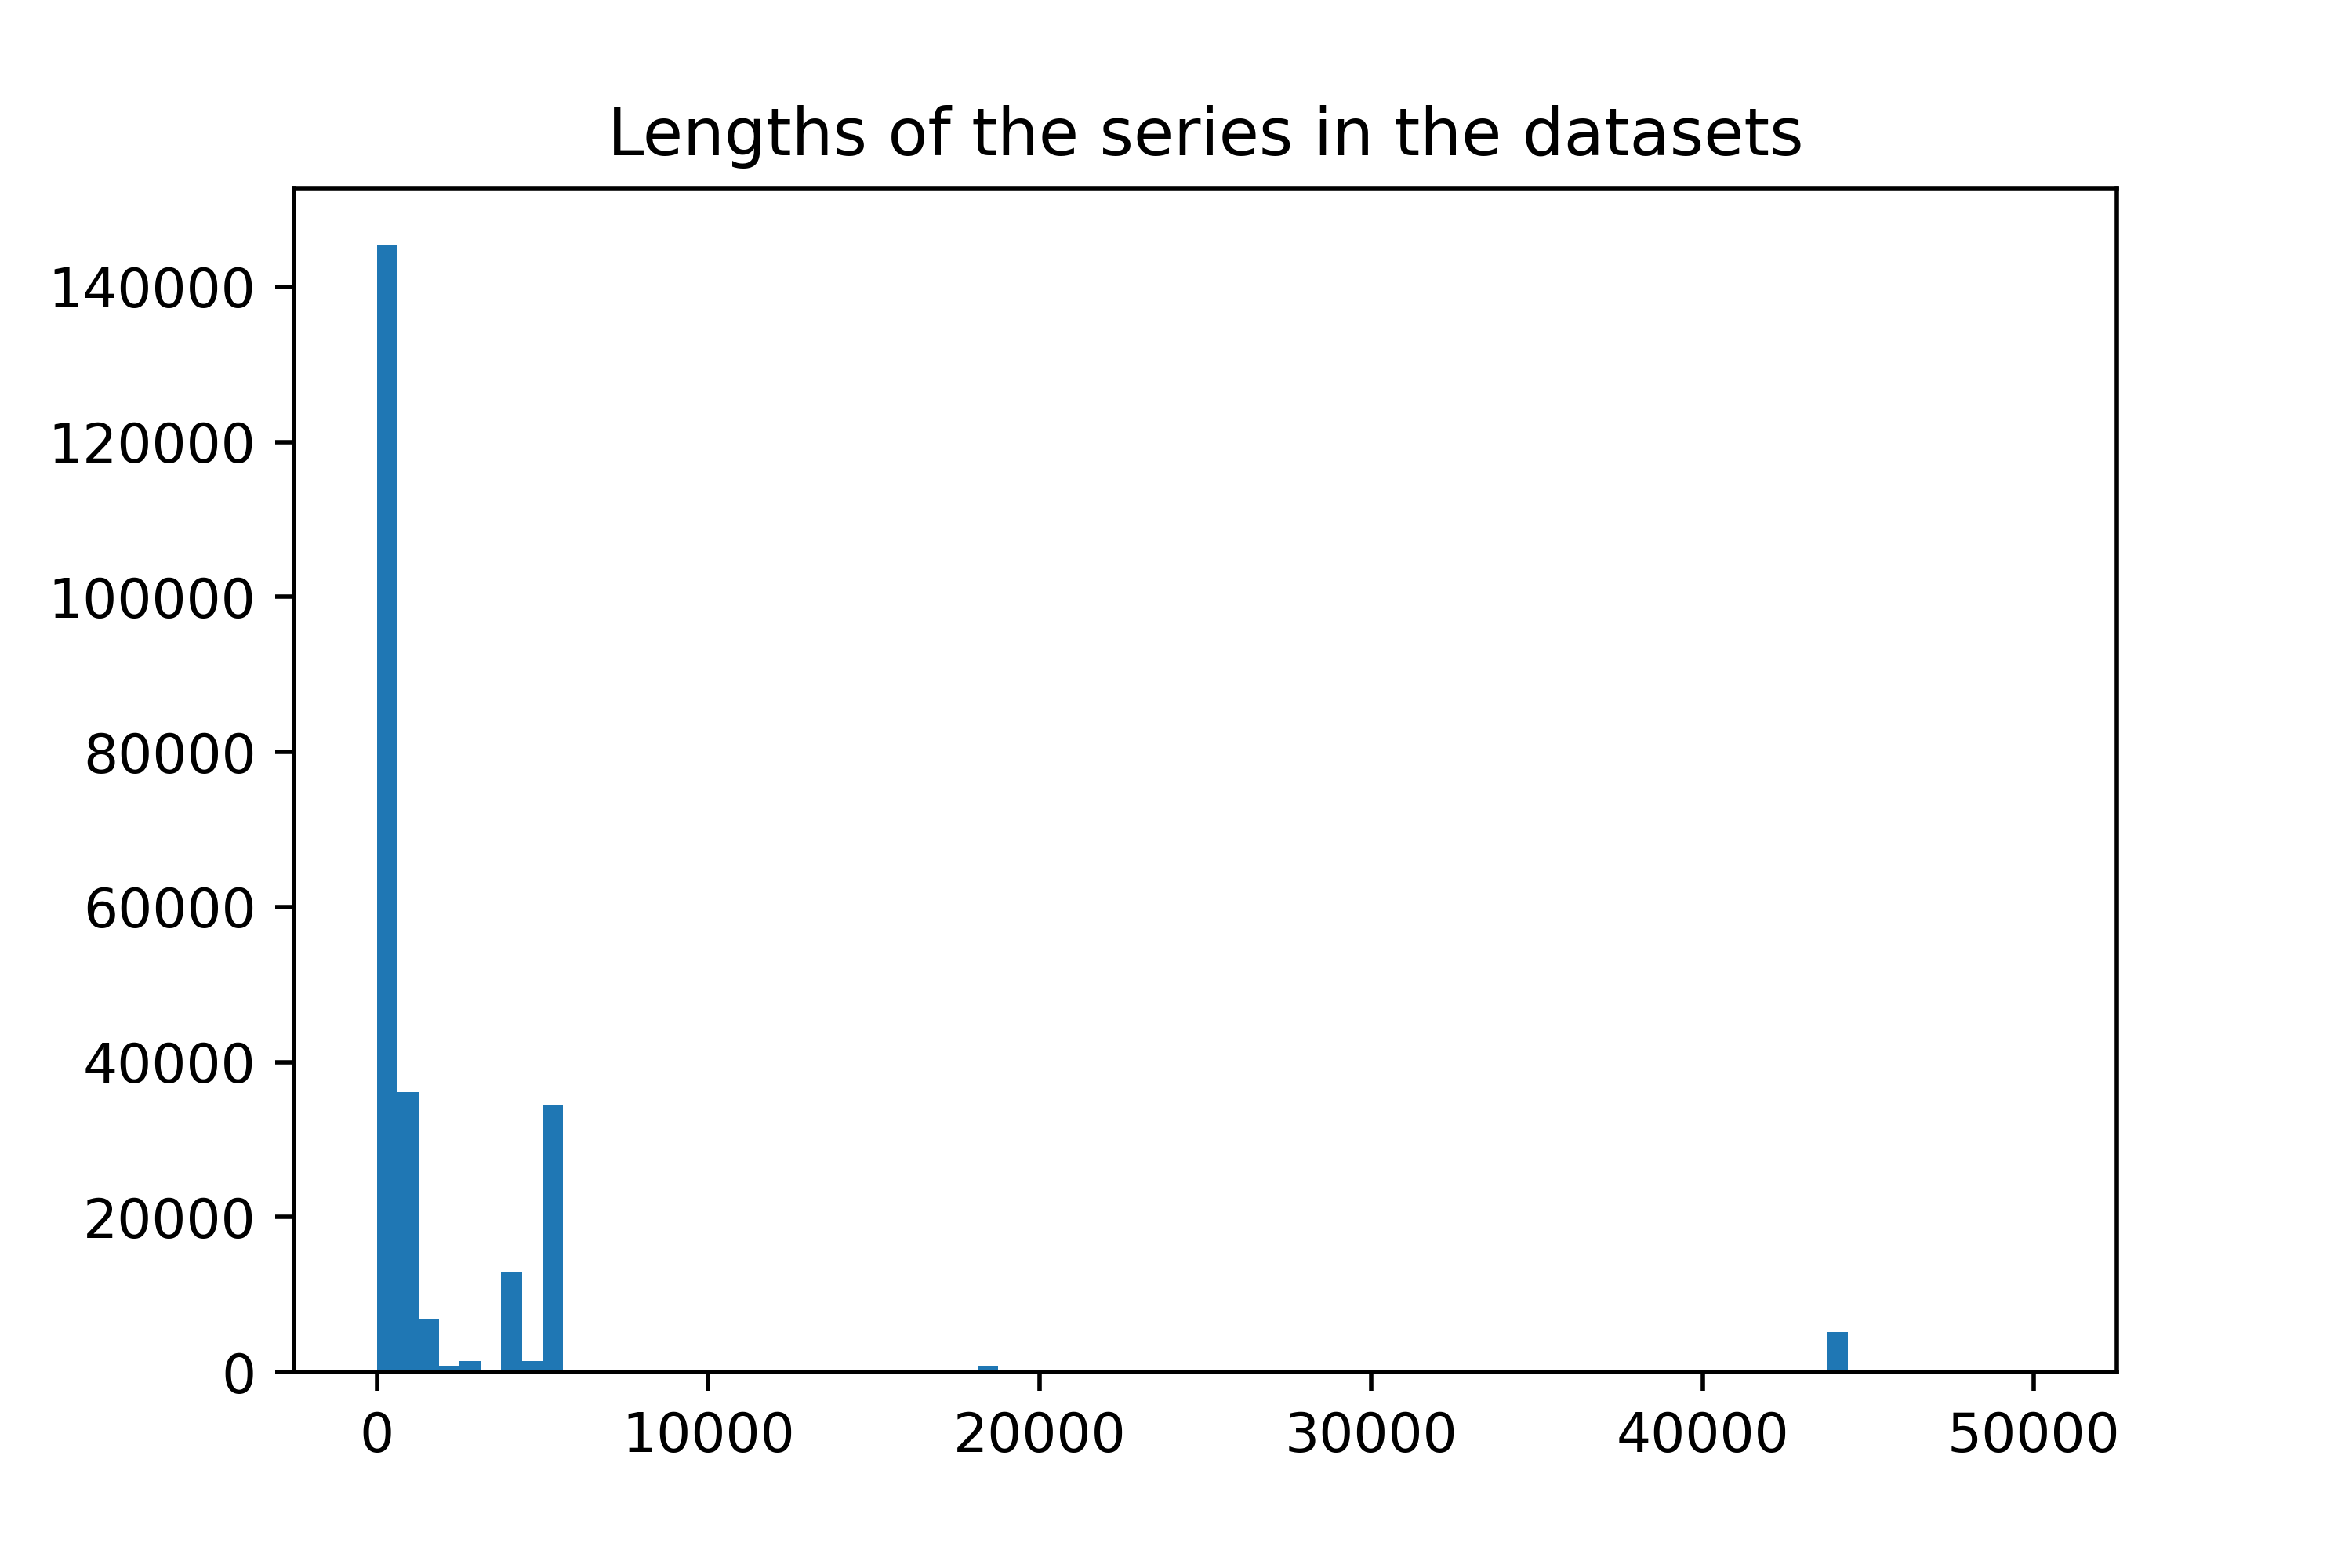
\includegraphics[width=7.9cm]{imgs/lengths_of_the_series_in_the_datasets.png}
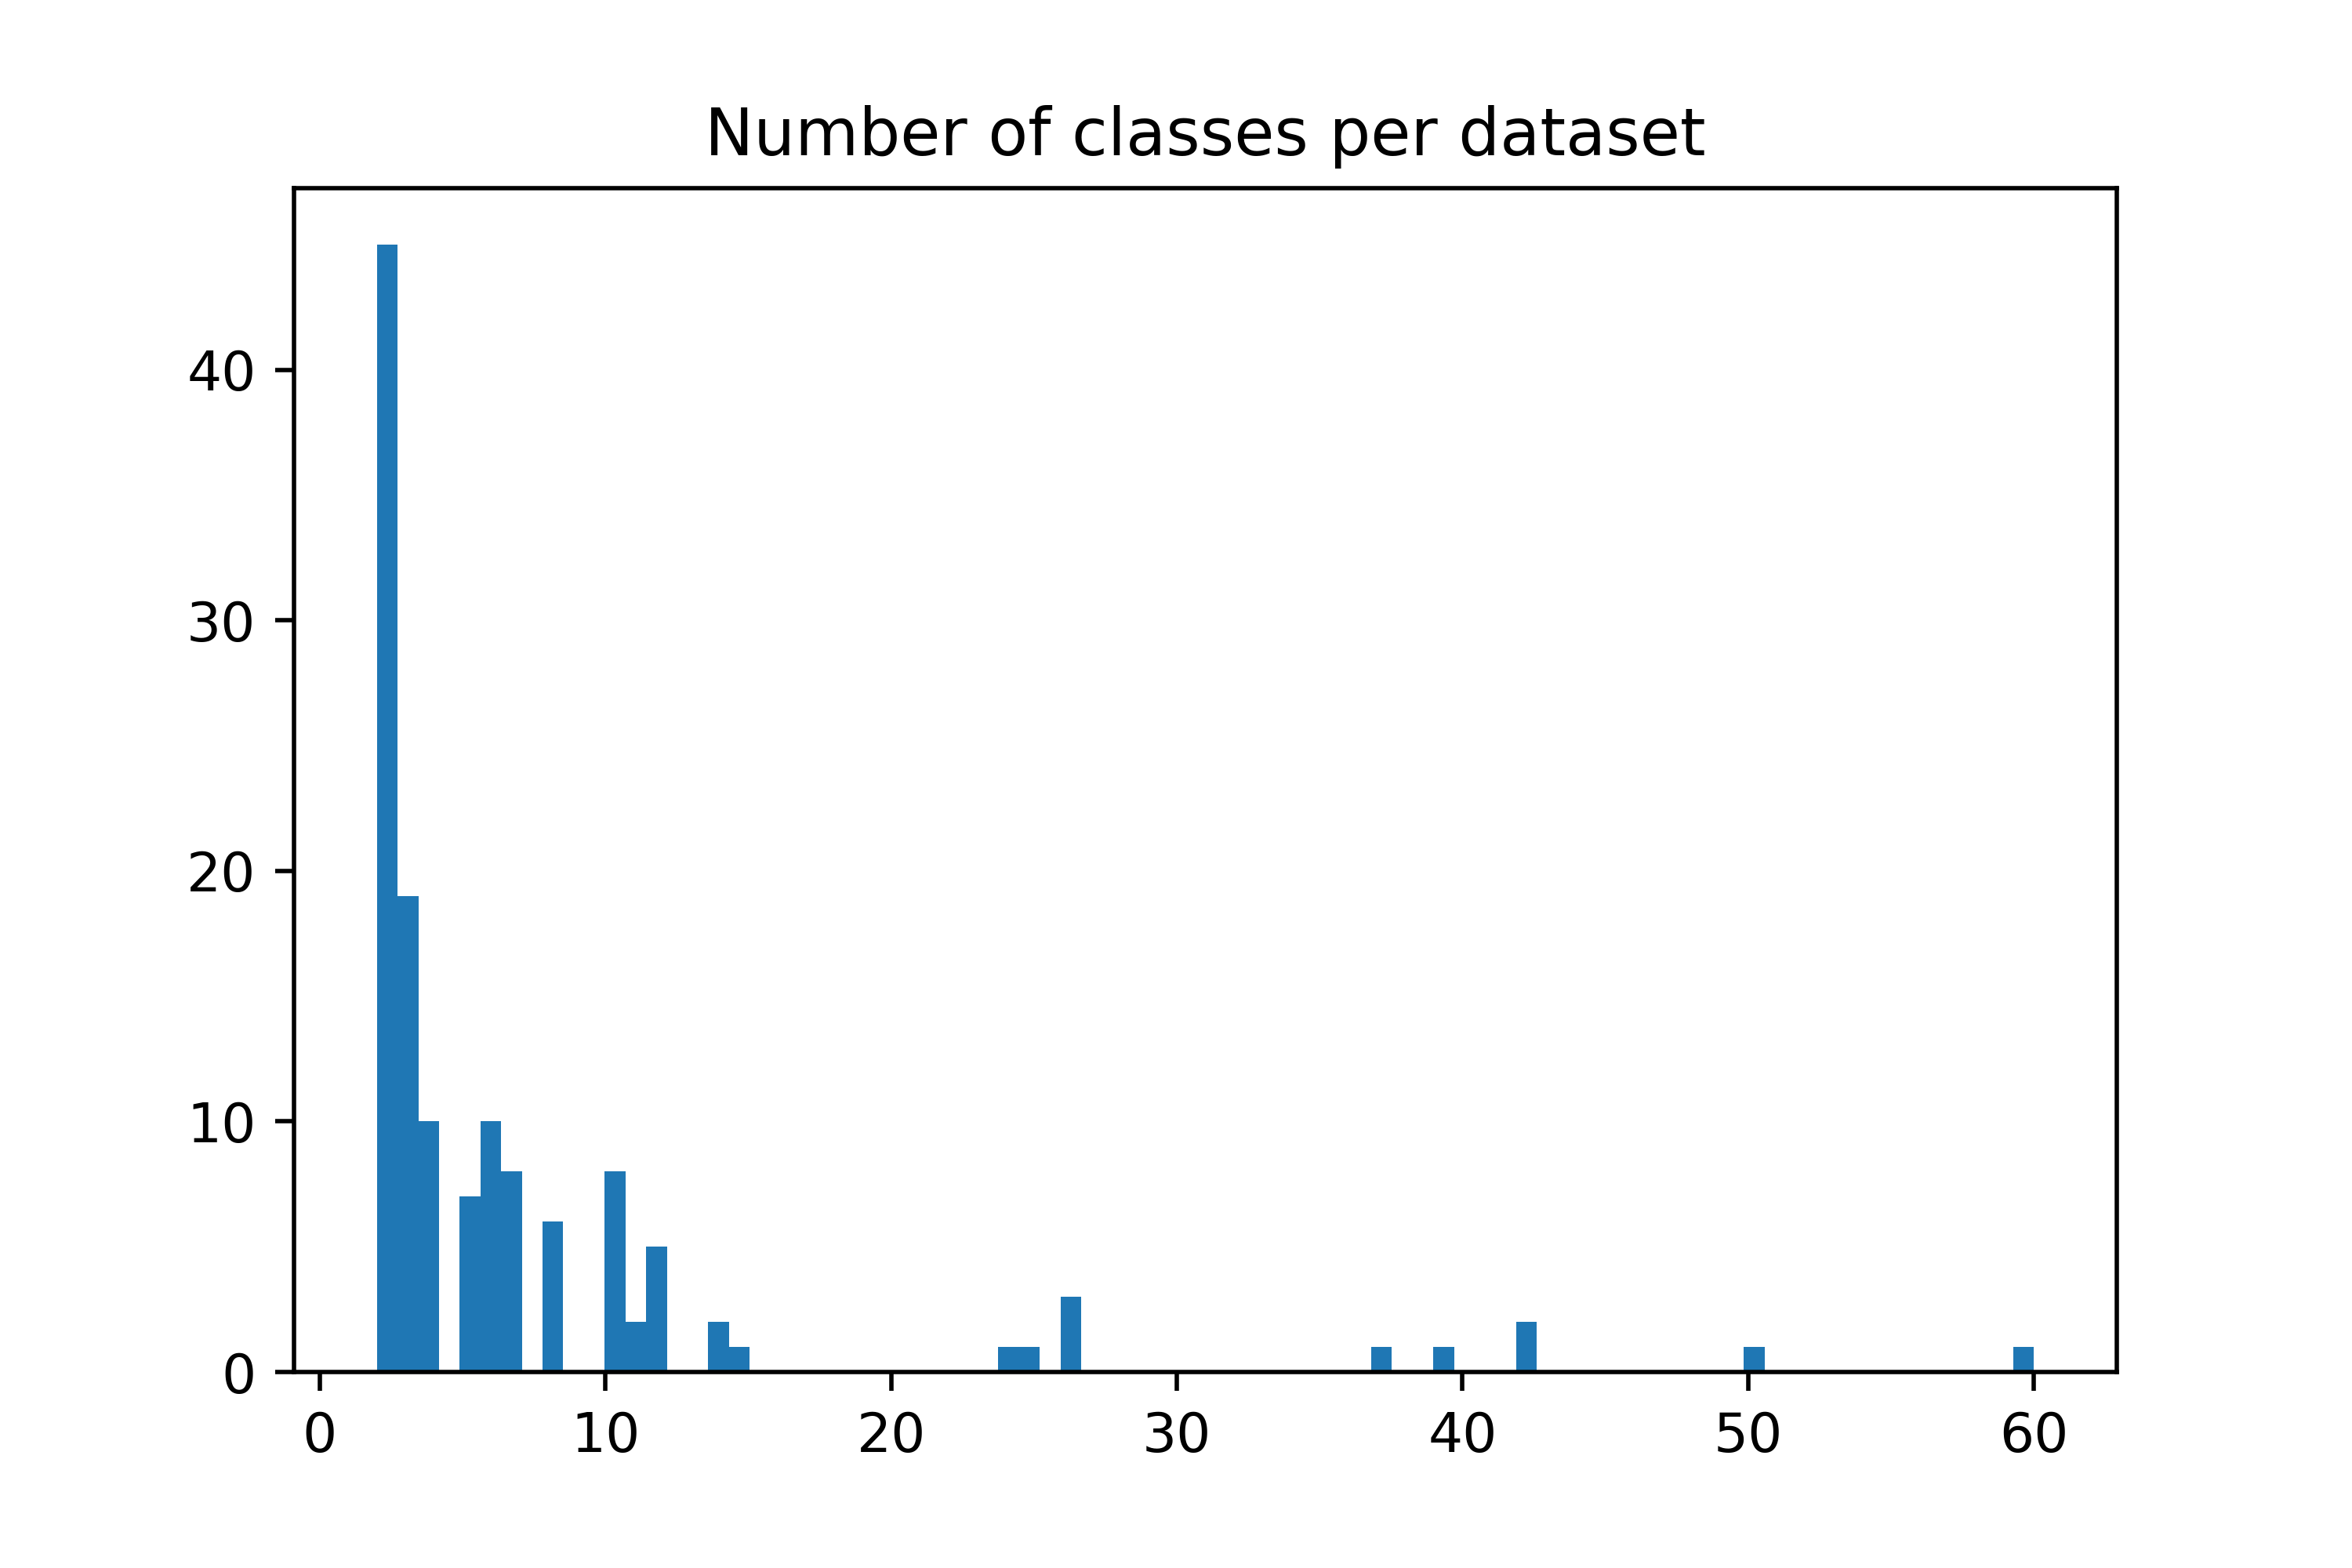
\includegraphics[width=7.9cm]{imgs/number_of_classes_per_dataset.png}
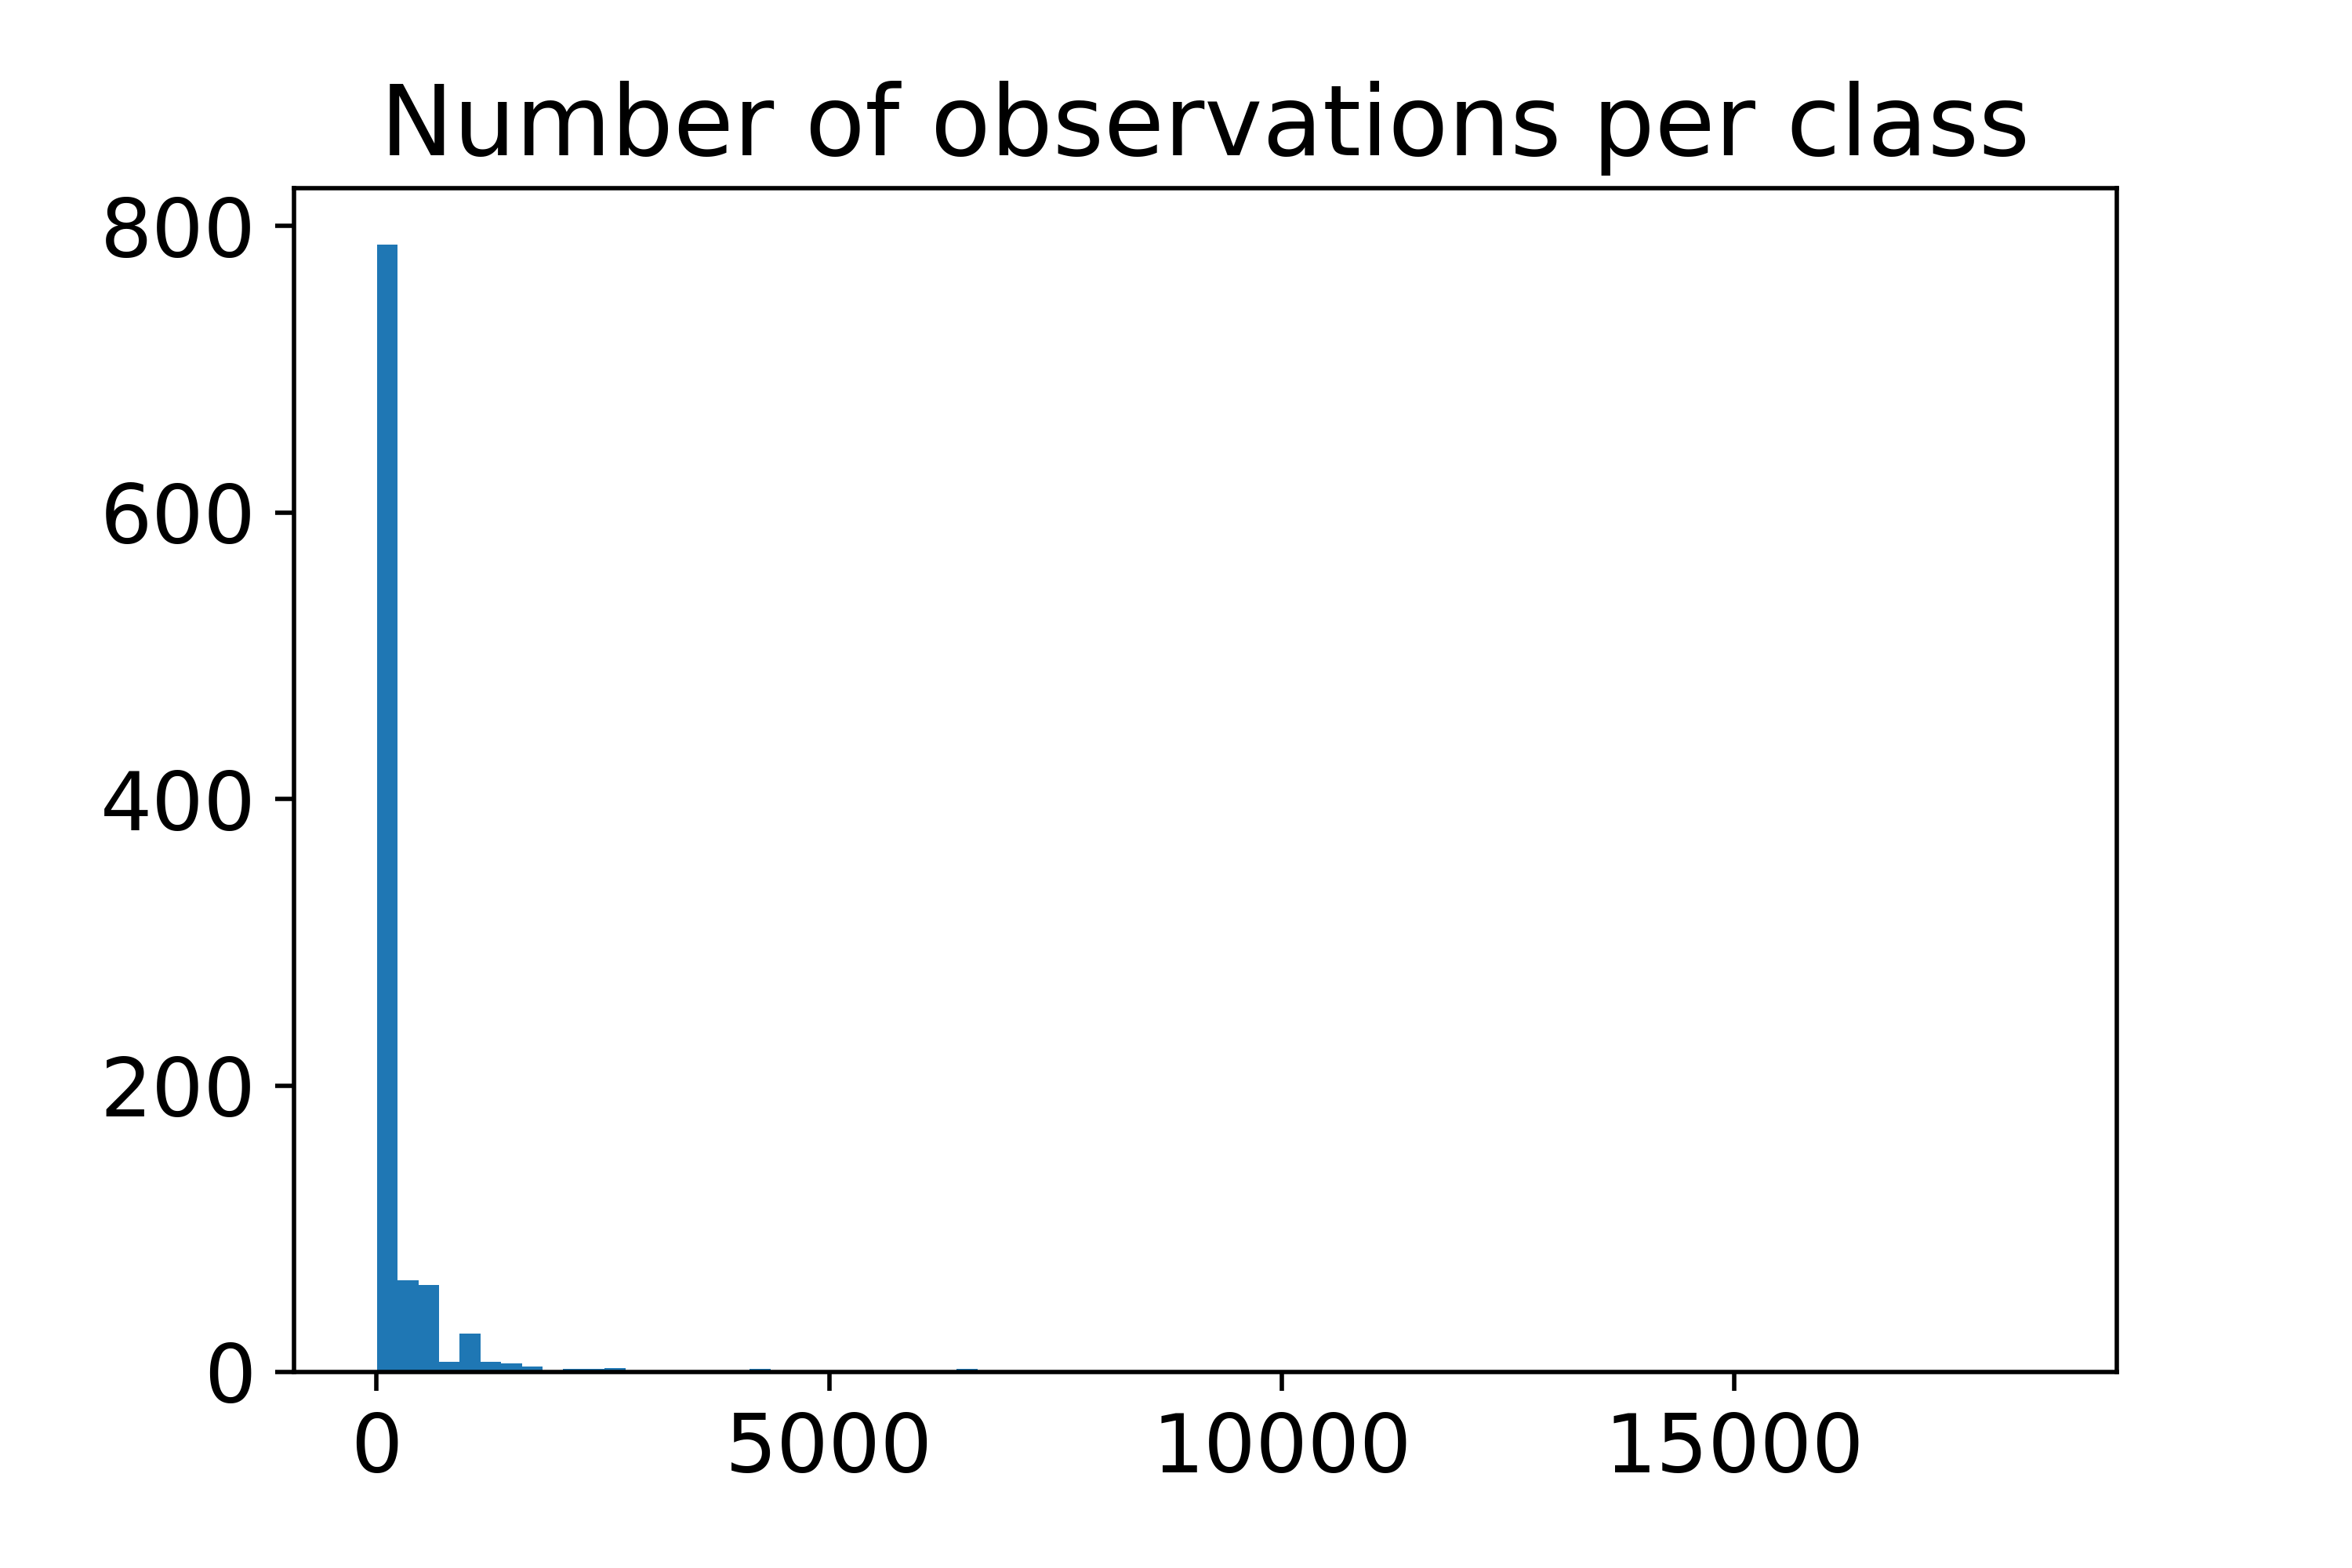
\includegraphics[width=7.9cm]{imgs/number_of_observations_per_class.png}
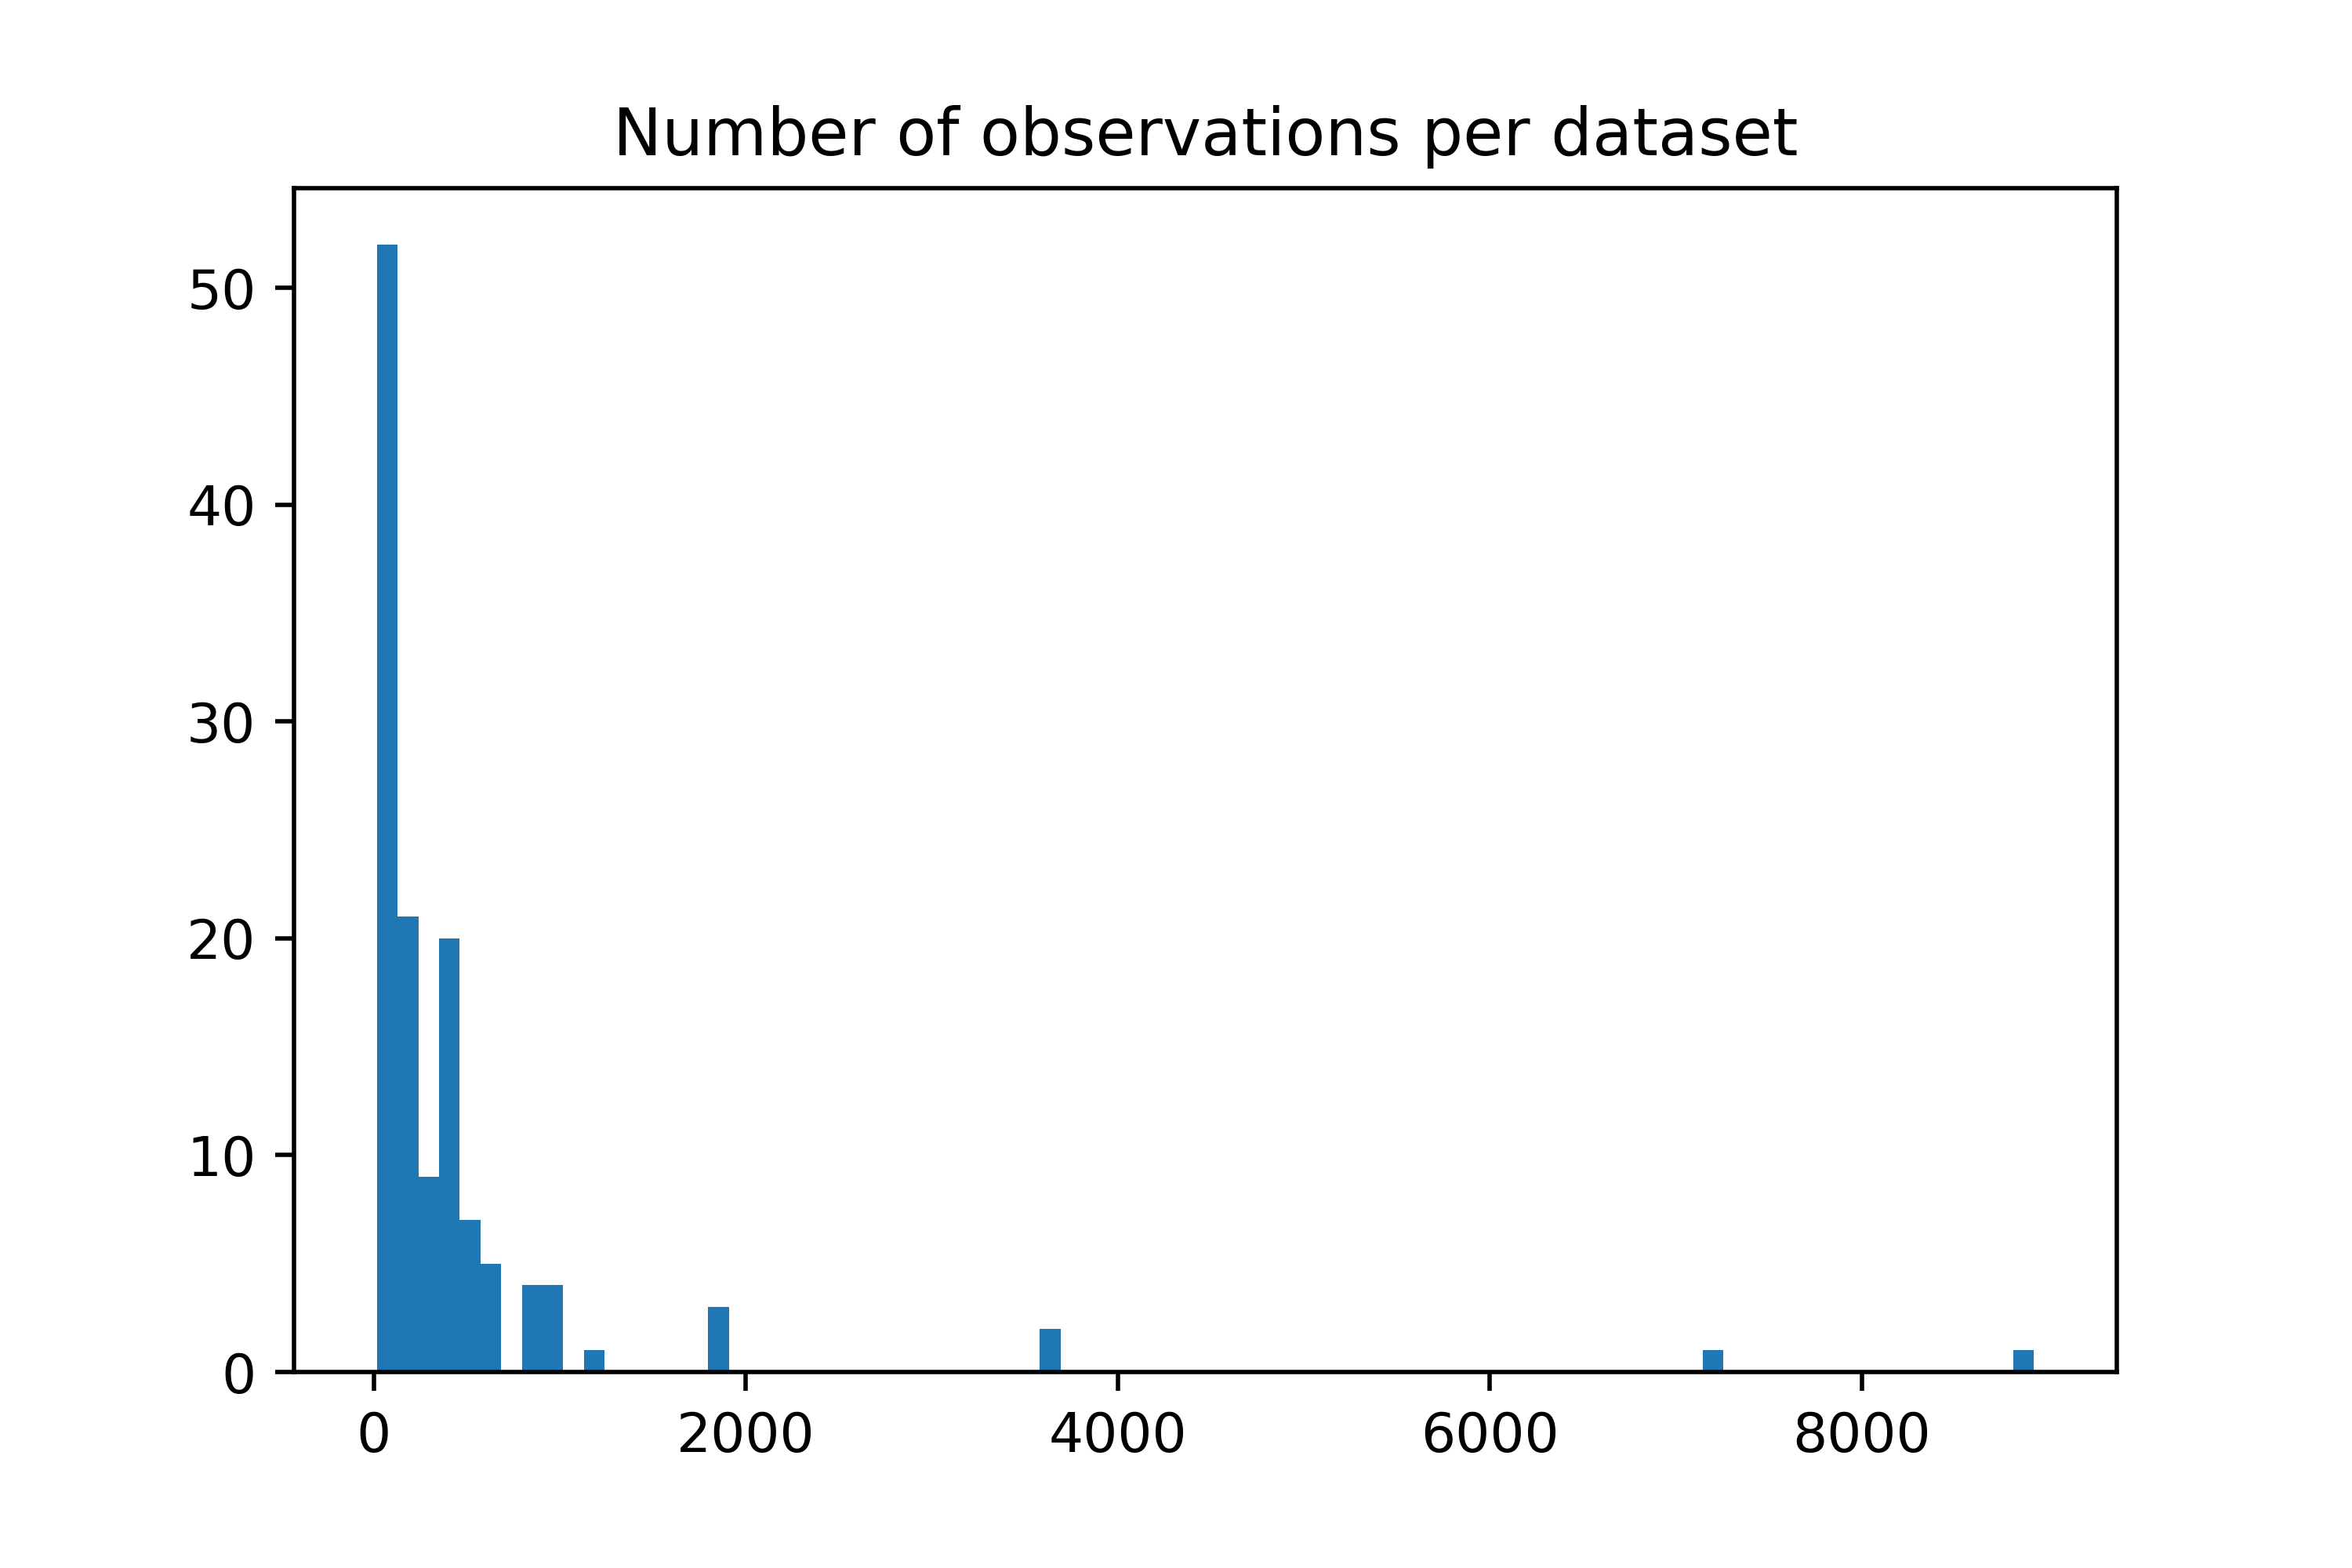
\includegraphics[width=7.9cm]{imgs/number_of_observations_per_dataset.png}
\caption{Summary of the UCR archive. The first plot is a histogram of time series length. The second histogram shows the number of classes in datasets. The two last histograms summarize the number of rows per class and per dataset.}  %TODO czcionka wieksza
\label{fig:histograms}
\end{figure}
The datasets in the archive are already split into train and test datasets. Most of the time, series are already z-normalized. However, the authors recommend testing on other test/train splits and preprocessing the time series accordingly to the method used. Below we describe the datasets in detail, considering all available categories.

\begin{itemize}
\item \textbf{Audio} - Sound amplitudes of heartbeats and spectrograms of sound produced by insects, cats, dogs, or whales. Classes represent normal and abnormal patients or different species.

\item \textbf{Device} - This category includes time series describing the power consumption of house devices or summarized population consumption for specific periods. This category is characterized by the combinations of spikes and constant areas in the time series. The data is divided into classes based on different types of devices or different time periods of data collection.

\item \textbf{ECG} - The data is composed of electrocardiogram readings. The classes correspond to different persons being examined, different diseases detected, the location of sensors, or the time when the data was collected.

\item \textbf{EOG} - There are two datasets describing electrooculograph readings, measuring the corneo-retinal standing potential between the front and the back of the human eye. The classes distinguish how the reading varied when writing and looking at different characters.
\item \textbf{EPG} - The electrical penetration graphs measure voltage changes in the electrical circuit that connects insects and their food source.
\item \textbf{Hemodynamics} - This category consists of time series representing airway, arterial blood, central venous, and pressure measurements. Each class represents one of the pigs that were examined.

\item \textbf{Image} - The majority of datasets in this category are outlines of images of different shapes. The images represent algaes, arrows, birds, bones, faces, vegetables, written words, fish, hands, and leaves. Another type of time series in this category are changes in the pixel intensity or growth of an area on a picture over time.

\item \textbf{Motion} - Positions of certain points (usually on the human body, but also on a car or worm) over an axis, e.g.,~while walking, speaking, driving, playing cricket, skating, writing, or performing gestures. One of the datasets uses electromyographic signals instead of point positions. Another dataset is different from others, as it describes the number of pedestrians at different hours.


\item \textbf{Sensor} - The data includes sensor readings, e.g.,~earthquake, humidity, temperature sensors, or robots. An example task is to predict an earthquake or to classify the surface the robot was walking on.

\item \textbf{Simulated} - The time series used in this category were simulated or obtained from an algorithm.

\item \textbf{Spectro} - This category consists mainly of food spectrograms but also one data set of time series representing  surface electromyography which captures the electric activity of groups of muscle at rest or during activity

\item \textbf{Traffic} - In this category are two datasets recording pedestrian flow. The classes correspond to weekdays or places.


\end{itemize}


\section{Preprocessing and augmenting time series}
Data preprocessing is the process of preparing, cleansing, and manipulating the data to optimize the training process. Data augmentation is a process used to increase the amount and variability of data. Data augmentation is beneficial when there is a limited amount of data, as it can prevent overfitting.

Many classical and deep learning models were invented and designed together with the data preprocessing and augmenting step \cite{bake_off, dl_tsc}. One such method is Window Slicing \cite{dl_tsc}. This method extracts subsequences of the original series. The resulting subsequences are then concatenated with a downsampled copy and smoothed copy. This method is used in Multi-scale Convolutional Neural Network \cite{multiscale} and Time Le-Net \cite{timelenet}.

Window Warping was another preprocessing and augmentation method proposed together with the former method in the Time Le-Net model. It aims at making the model more robust to perturbations in the time axis by training the network on \textit{squeezed} or \textit{dilated} series together with the original series. The \textit{dilated}/\textit{squeezed} time series is two times longer/shorter than the original time series.
The dilated, squeezed, and original time series are concatenated, forming a vector 3.5 longer than the original time series. In the Time Le-Net model, this vector undergoes the Window Slicing preprocessing step before training.



\section{Transfer learning}
Transfer learning is a technique that attempts to apply knowledge learned  while solving one task to enhance the learning process for another task. Formally, the problem can be described using the notions of tasks and domains \cite{survey_transfer_learning, comp_survey_transfer_leaerning}. A \textit{Domain} is a pair $\mathcal{D}=(\mathcal{X}, P(\mathcal{X}))$, where $\mathcal{X}$ is the feature space (e.g.,~the time series observations, and $P(\mathcal{X})$ is the probability distribution over the feature space. A \textit{Task} is a pair of label space $\mathcal{Y}$ and the decision function $f$, $\mathcal{T} = (\mathcal{Y}, f)$. The decision function $f$ is learned from $\mathcal{X}, P(\mathcal{X}), \mathcal{Y}$ in the learning process.

Transfer learning attempts to utilize knowledge from different domain/domains and task/tasks. Formally, given $S \in \natur$ source domains and source tasks ($\{(\mathcal{D}_i^S,\mathcal{T}_i^S): i=1, \dots, S \}$) and $T \in \natur$ target domains and target tasks ($\{(\mathcal{D}_i^T,\mathcal{T}_i^T): i=1, \dots, S \}$) transfer learning utilizes knowledge learned from source domains and tasks to improve the learning process of decision functions in target tasks $\mathcal{T}_i^T$
\subsection{Transfer learning categorization}
Transfer learning can be categorized from different points of view \cite{comp_survey_transfer_leaerning}. One of the ways in which we can divide transfer learning algorithms is based on the availability of the labels:
\begin{itemize}
\item \textbf{inductive} transfer learning - labels are available for both source and target datasets
\item \textbf{transductive} transfer learning - labels are available only in the domain dataset
\item \textbf{unsupervised} transfer learning - no labels available in either dataset
\end{itemize}
Another way of dividing transfer learning methods is by comparing feature space distribution and labels. If the source and training dataset consists of the same features, belonging to a similar distribution ($\mathcal{D^S} = \mathcal{(X, P(X))^S} = \mathcal{(X, P(X))^T} = \mathcal{D^T})$) and the label spaces are equal ($\mathcal{Y^S} = \mathcal{Y^T} $), then the task can be described as homogeneous transfer learning. If at least one of the former assumptions does not hold, the transfer learning setting is heterogeneous.

Transfer learning can be categorized based on the algorithm/approach used. There are four main categories \cite{deep_tranfer_learning} used in deep learning:
\begin{itemize}
	\item \textbf{instance} based transfer learning - target dataset is enriched by instances from the source dataset belonging to the target distribution.
	\item \textbf{mapping} based transfer learning - source and target dataset are mapped to one domain. The distribution is adjusted in both datasets.
	\item \textbf{network} based transfer learning - target classifier uses parts of the network from the source classifier $f$.
	\item \textbf{adversarial} based transfer learning - an adversarial network tries to distinguish between the two datasets. If the network fails at this task, then it means that the extracted features are similar between source and target datasets.
\end{itemize}

\subsection{Characteristics of a good source domain}

In the field of image processing, it is widespread to use convolutional neural networks \mbox{pre-trained} with the ImageNet dataset \cite{imagnet}.  ImageNet is a large dataset of human-annotated images. It contains 1 million labeled images of 1000 classes. The label space consists of fine-grained classes such as breeds of dogs and cats and coarse-grained classes like \textit{red wine} and \textit{traffic light}. Example pictures from this dataset are shown below \ref{fig:image_net}. As transfer learning based on this dataset became more popular and successful, a question arose: Which features of this dataset make it so suitable for this task?
\FloatBarrier

\begin{figure}[h!]
\centering
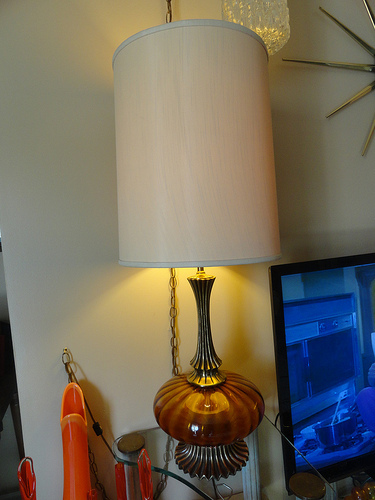
\includegraphics[height=5cm]{imgs/lamp.jpeg}
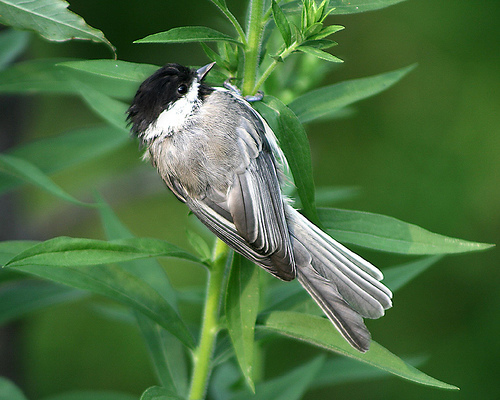
\includegraphics[height=5cm]{imgs/bird1.jpeg}
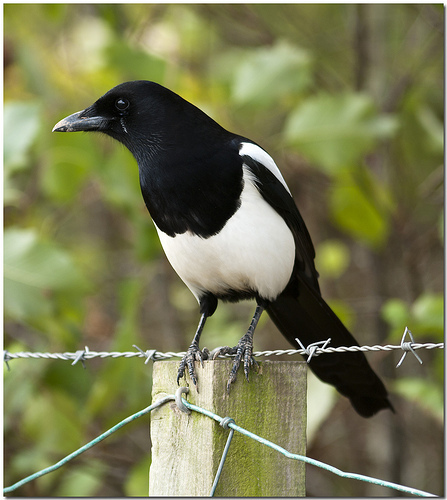
\includegraphics[height=5cm]{imgs/bird2.jpeg}
\caption{Sample images from the ImageNet dataset, with examples of similar (fine-grained) classes like two birds of different breeds and coarse-grained classes, like a lamp and a bird. \href{https://www.kaggle.com/competitions/imagenet-object-localization-challenge/data}{Source: url}}
\label{fig:image_net}
\end{figure}

\FloatBarrier

A study conducted in \cite{imagnet} attempts to answer this question. The first hypothesis is that the volume of the dataset is relevant to train accurate, general classifiers. The authors compared models that were pretrained on the original dataset and those based on sampled subsets (reduced 2, 4 8 and 20 times). The results show that the more training examples, the better results. The accuracy of the initial classifier occurred to be more dependent on the size of the dataset than the accuracy of classifiers fine-tuned from the base classifier. It is natural that the base classifier's accuracy depends on the dataset size. Still, the classifier fine-tuned from the base classifier seems to cope with the reduced dataset, and the impact on the accuracy is less detrimental. This is visible in Figure \ref{fig:size_acc_img}.

\FloatBarrier


\begin{figure}[h!]
\centering
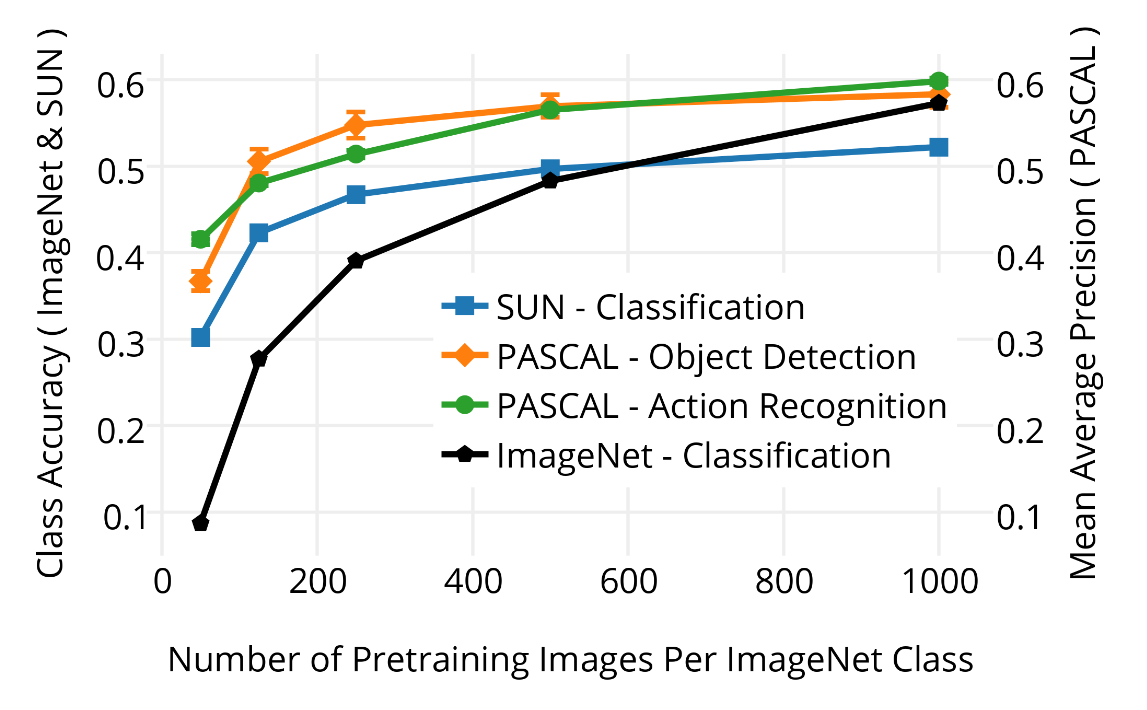
\includegraphics[width=10cm]{imgs/imagenet_instances_accuracy.png}
\caption{Accuracy of the base classifier (black) and classifiers fine-tuned from the base classifier. Image source: \cite{imagnet}}
\label{fig:size_acc_img}
\end{figure}
\FloatBarrier

Next experiments examine the label space. The authors study if the granularity of the label space is essential for the problem. To compare the results, the label space is clustered, and 127 classes are derived from the initial 1000 classes. Pre-training with the reduced label space has a minimal negative impact on the accuracy of classifiers fine-tuned from this classifier. This suggests that such a fine division may not be needed.

Finally, the last question is if we train the classifier on the reduced label space with 127 classes, will it be able to distinguish between the fine-grained classes? To examine that, the authors extracted features from the first layers of the networks trained on reduced label space. Then, the authors performed classification with 1-NN and 5-NN models on the extracted feature space but with 1000 classes. The findings are that the k-NN classifier performs $15\%$ worse on a reduced dataset versus the normal dataset.

While the article \cite{imagnet} does not conclude which single feature of the ImageNet dataset makes it so efficient as a source dataset for transfer learning, it is clear that all properties of this dataset are essential for the accuracy of the classifier. We try to recreate the properties of the ImageNet dataset when creating the source dataset from time series.



\subsection{Negative transfer in naive transfer learning approach}\label{Negative_transfer}
Negative transfer is a problem in the transfer learning process when the target classifies achieve worse accuracy than without using transfer learning. Transfer learning for time series has been investigated in \cite{transfer_learning_time_series}. The paper's authors tested transfer learning on all datasets from the UCR archive. In the first approach, called \textit{naive transfer learning}, the authors used all pairs of datasets. One dataset from the pair was used as a source dataset to prepare the source classifier for transfer learning. The second dataset was used to fine-tune the former classifier. The architecture used in this approach was the Fully Convolutional Network, described in section \ref{FCN}.  All layers except for the last one were transferred from the source classifier to the target classifier. The authors compared the accuracy of a fine-tuned classifier to that of a classifier trained without transfer learning.

With respect to different source datasets, target classifiers' accuracies exhibited a high variance. There were cases where the fine-tuned classifiers suffered from transfer learning. On the other hand, for each target dataset, there was always a source dataset beneficial for the classification results. It is shown in the picture \ref{fig:tr_learning_min_max}, where for each target dataset, the maximum, median, and minimum accuracies for the different experiments were plotted.

\FloatBarrier


\begin{figure}[h!]
\centering
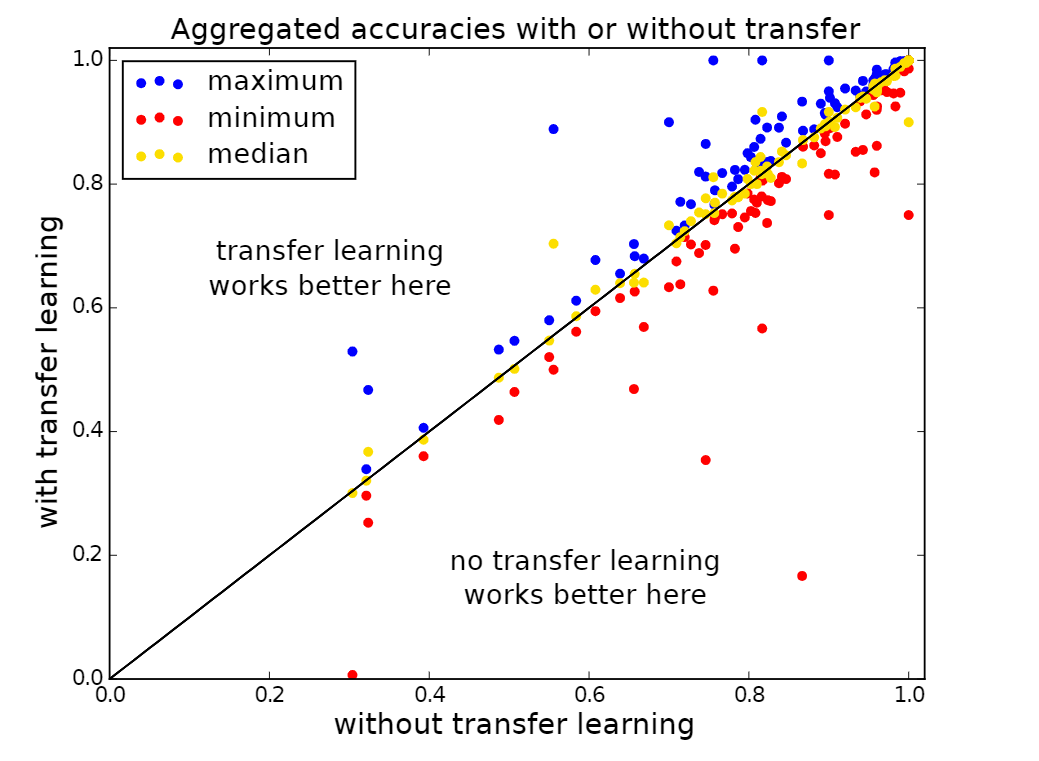
\includegraphics[width=10cm]{imgs/max_min_transfer_learning.png}
\caption{Image source: \cite{transfer_learning_time_series}}
\label{fig:tr_learning_min_max}
\end{figure}
\FloatBarrier
A negative transfer learning effect can be minimized or avoided by optimally choosing the source dataset/datasets. To improve the transfer learning process, the authors proposed a method of choosing the source dataset based on the DTW distance. This method is described in \ref{DTW_choosing}.

\subsection{Inter-dataset similarity measure based on Dynamic Time Warping Barycenter Averaging} \label{DTW_choosing}
Choosing the source dataset for transfer learning randomly or by trial and error can lead to the \textit{Negative transfer} problem, described in the previous chapter (\ref{Negative_transfer}). In \cite{transfer_learning_time_series}, the authors proposed an inter-dataset similarity measure that is used to choose the source dataset for transfer learning optimally. The first step of the method is to compute a \textit{prototype} time series per each class for every considered dataset. This step reduces the volume of the data that is used in the next step. The next step is to compute the distances between each pair of datasets, choosing the minimum DTW distance between prototypes of each class in both datasets. We proceed to describe the algorithm in detail below.

The algorithm uses DTW barycenter averaging \cite{dtw_dba}. The result of this method is a times series that minimizes the sum of DTW distances to each time series from the dataset.
$$DTW\_average = \arg\min_{X \in  2^{\real}}  \sum_{\bar{X}\in \mathcal{X}} DTW(X, \bar{X})$$
The resulting time series does not need to belong to the original dataset $\mathcal{X}$.

The first step of the algorithm is the data reduction step. For each class in the dataset $\{(X_i, y_i): i=1, \dots , N\}$, $y_i=c \in \{ 1, \dots, C\}$ the prototype time series $P_c$ is defined as the result of DTW barycenter averaging performed on the subset of $\mathcal{X}$ corresponding to class $c$. As a result, the original dataset is reduced to $C$ observations.


%\pagebreak
The next step is to compute the distance between the target dataset and all possible source datasets. The distance between two datasets is the minimum DTW distance between each pair of prototypes from the reduced datasets. The whole algorithm is described in detail in \cite{transfer_learning_time_series}.

In \cite{transfer_learning_time_series}, the distance was computed pairwise for all available datasets (using train splits). The authors compare the transfer learning performance with a randomly chosen source dataset versus choosing the source dataset that minimizes the former distance to the target dataset. The results are shown below (Figure \ref{fig:smart_transfer_learning}).
\FloatBarrier


\begin{figure}[h!]
\centering
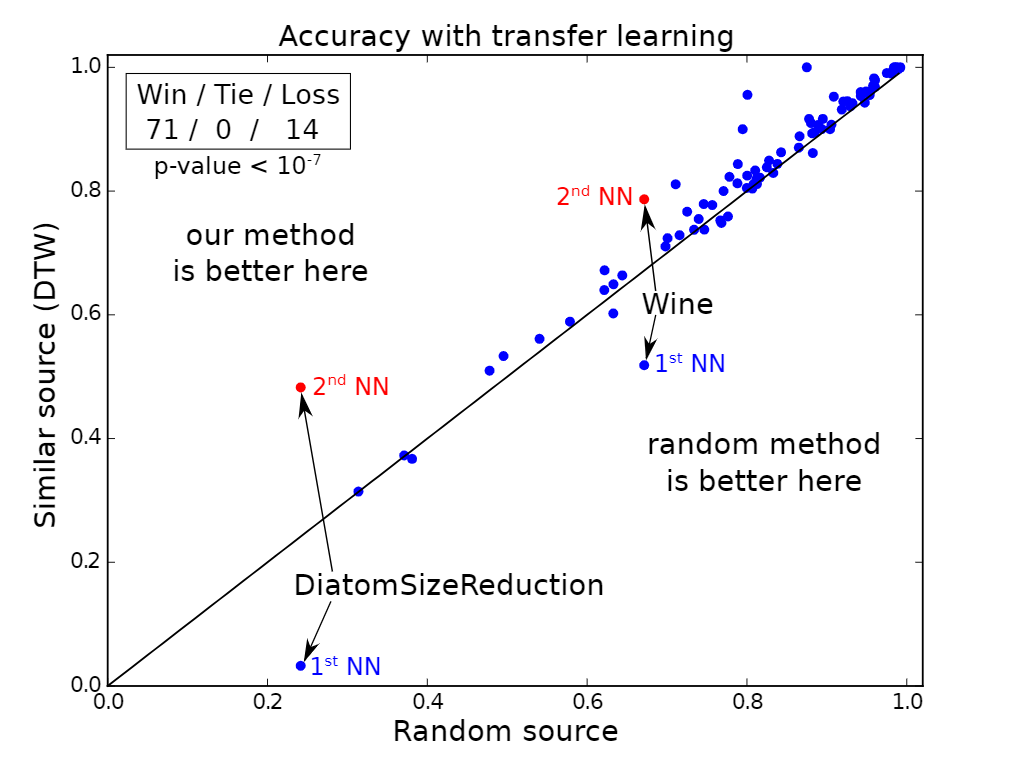
\includegraphics[width=10cm]{imgs/smart_transfer_learning.png}
\caption{Image source: \cite{transfer_learning_time_series}}
\label{fig:smart_transfer_learning}
\end{figure}
\FloatBarrier

The result shows that choosing the source dataset for transfer learning based on similarity to the target dataset may lead to benefits. In this work we try to construct the dataset artificially, by combining, preprocessing, and augmenting the datasets from the UCR archive, to mimic the properties of the ImageNet dataset. The artificial dataset is composed of multiple datasets. Therefore we rather won't use this similarity to choose one particular dataset. We take the inter-dataset distance into account when adjusting the distribution of classes in the artificial dataset, to favour classes similar to the target dataset.

\chapter{Methodology}
In this chapter, we cover the technical implementation of the solution. We introduce methods that aim at inductive transfer learning for time series classification. Most importantly, we introduce two approaches to multi-source transfer learning - the \textit{baseline} and the \textit{ensemble} approach. We also cover a selection method for selecting the source datasets given a target dataset. We also briefly summarize data reading and preprocessing steps.

\section{Data reading}\label{section:reading}
The data downloaded from the UCR archive is available in two formats, \texttt{ts} (as text files) and \texttt{arff/weka} (as binaries). In order to speed up the reading and conversion time, all datasets were read, concatenated, and saved as one array of time series (the original lengths were preserved). At this point, only basic preprocessing was done. It included the following steps:
\begin{itemize}
\item replacing \texttt{NaN} values with zeros
\item removing zeros at the end of the time series. This step was done because some of the time series published in the UCR archive were already padded with zeros to have the same lengths. This assumption is not necessary when using a Fully Convolutional Network.
\item trimming the series if the time series length exceeded $50 000$ time steps (applies only for one dataset - \texttt{DuckGeese}).


\end{itemize}

All time series were concatenated to one array of series and saved in a \texttt{.npy} format.


\section{Preprocessing and preparing the data}\label{section:preprocessing}
 In order to avoid focusing on one particular form of preprocessing and preparing the data, the preprocessing was done on the fly when training the data. This way, fast experimenting with hyperparameters and methods was possible. In order to achieve it, Keras DataGenerators were used. DataGenerators allow for defining a Python generator that provides batches of data to the fit method instead of providing a fixed dataframe. Using DataGenerators was useful when dealing with datasets consisting of time series of variable lengths and Fully Convolutional Networks. In such case, the time series lengths could differ for each batch.
For the Fully Convolutional Networks, we implemented \texttt{VariableLengthDataGenerator}.
The preprocessing steps are described below:
\begin{itemize}
   \item selecting time series to the batch. The number of series in a batch was equal to $32$. The series were chosen so that the classes were uniformly distributed in the batch by resampling.
   \item normalizing the time series values to standard normal distribution. The normalization is done per one time series
   \item obtaining time series of the same length within the batch. The length of the longest series in the batch is computed. The target length is equal to the length of the longest series or $3000$ if it exceeds. If a time series in the batch is shorter than the target length, then the series is padded with zeros.

\item augmentation - $30\%$ of the series in a batch are flipped over the x or y axis with $50\%$ chance.

\end{itemize}

\section{Neural network architectures}
The experiments were conducted on the Fully Convolutional Network. The network's detailed architecture summary, including layer sizes, is shown below. \begin{verbatim}
Model: "FCN"
_________________________________________________________________
 Layer (type)                Output Shape              Param #
=================================================================
 input_1 (InputLayer)        [(32, None, 1)]         0

 conv1d (Conv1D)             (32, None, 128)         1536

 batch_normalization (BatchN  (32, None, 128)        512
 ormalization)

 activation (Activation)     (32, None, 128)         0

 conv1d_1 (Conv1D)           (32, None, 256)         164096

 batch_normalization_1 (Batc  (32, None, 256)        1024
 hNormalization)

 activation_1 (Activation)   (32, None, 256)         0

 conv1d_2 (Conv1D)           (32, None, 128)         98432

 batch_normalization_2 (Batc  (32, None, 128)        512
 hNormalization)

 activation_2 (Activation)   (32, None, 128)         0

 global_average_pooling1d (G  (32, 128)              0
 lobalAveragePooling1D)

 dense (Dense)               (32, 2)                 258

=================================================================
Total params: 266,370
Trainable params: 265,346
Non-trainable params: 1,024
\end{verbatim}
The second parameter in output shape is always equal to \texttt{None}, because the time series length in a batch is not known in advance.
\section{Hyperparameters}\label{section:hyperparameters}
The hyperparameters used for the training were identical for all experiments. The hyperparameters were usually left as default. We did not experiment with hyperparameter optimization as we focused on the transfer learning approach. The most important hyperparameters are shown in the table \ref{table:hyperparams}.

\FloatBarrier

\begin{table}[!h]
\centering
\tabcolsep=0.11cm
\scalebox {0.9}{
\begin{tabular}{@{}|l|l|@{}}



\toprule
\textbf{Hyperparameter}       & \textbf{value} \\ \midrule
Batch size                                & 32 \\ \midrule
Augmentation rate  & 0.3\\ \midrule
Learning rate                                 & 1e-5 with 0.75 decay over 10 000 steps (exponential decay) \\
\\ \midrule
Number of epochs                                & 10\\
\bottomrule
%\end{singlespace}
\end{tabular}
}
\caption{Summary of hyperparameters.}
\label{table:hyperparams}
\end{table}
\FloatBarrier
\section{Multi-source transfer learning}
As single-source transfer learning for time series classification was covered by Fawaz et al.~\cite{transfer_learning_time_series}, this thesis considers mainly transfer learning using multiple source datasets. Two transfer learning approaches were developed, named \textit{baseline approach} and \textit{ensebmle approach}. Both of them are described below. Both of those approaches consider multiple (the number is arbitrary) source datasets, single target dataset, the same neural network architectures, and hyperparameters.

\section{Baseline approach}\label{section:baseline}
The \textit{baseline approach} is a simple extension to the classical transfer learning approach used in deep learning. Usually, in deep learning, the neural network is first trained on a large, diverse dataset (like ImageNet). The network is usually trained on the source dataset, and then the first layers are used in the source classifier.

The idea here is similar, but the source dataset is created artificially from multiple datasets. As most of the datasets in the UCR archive are small, we concatenate them to obtain a bigger dataset. Suppose that we have $N$ datasets $(X_i^\mathcal{S}, Y_i^\mathcal{S})$, $i=1, \cdots, N$.
The pre-training dataset $(X^\mathcal{T}, Y^\mathcal{T})$ is created as follows:
$X^\mathcal{T} = \bigcup_{i=1}^N X_i^\mathcal{S}$,

$Y = \{prefix_i(y): y \in Y_i, i=1, \dots, N\}$
where $prefix_i(\cdot)$ is a function such that $$\forall_{i\neq j} \forall_{\bar{y} \in Y_i, \hat{y} \in Y_j} \ \  prefix_i(y) \neq prefix_j{y}$$
In our case, the prefix function given a class name (as a string) transforms the string by adding a prefix with the dataset name. This way, the classes remain distinct after concatenation. The number of classes in the resulting dataset is equal to the sum of the number of classes in each dataset. The examples that correspond to the same dataset should be intuitively similar to each other (analog of the fine-grained classes in ImageNet), while examples from different datasets cover more latent space (analog of the coarse-grained classes in ImageNet). The concatenation process is shown in Figure \ref{fig:baseline_dataset}


\FloatBarrier
\begin{figure}[h!]
\centering
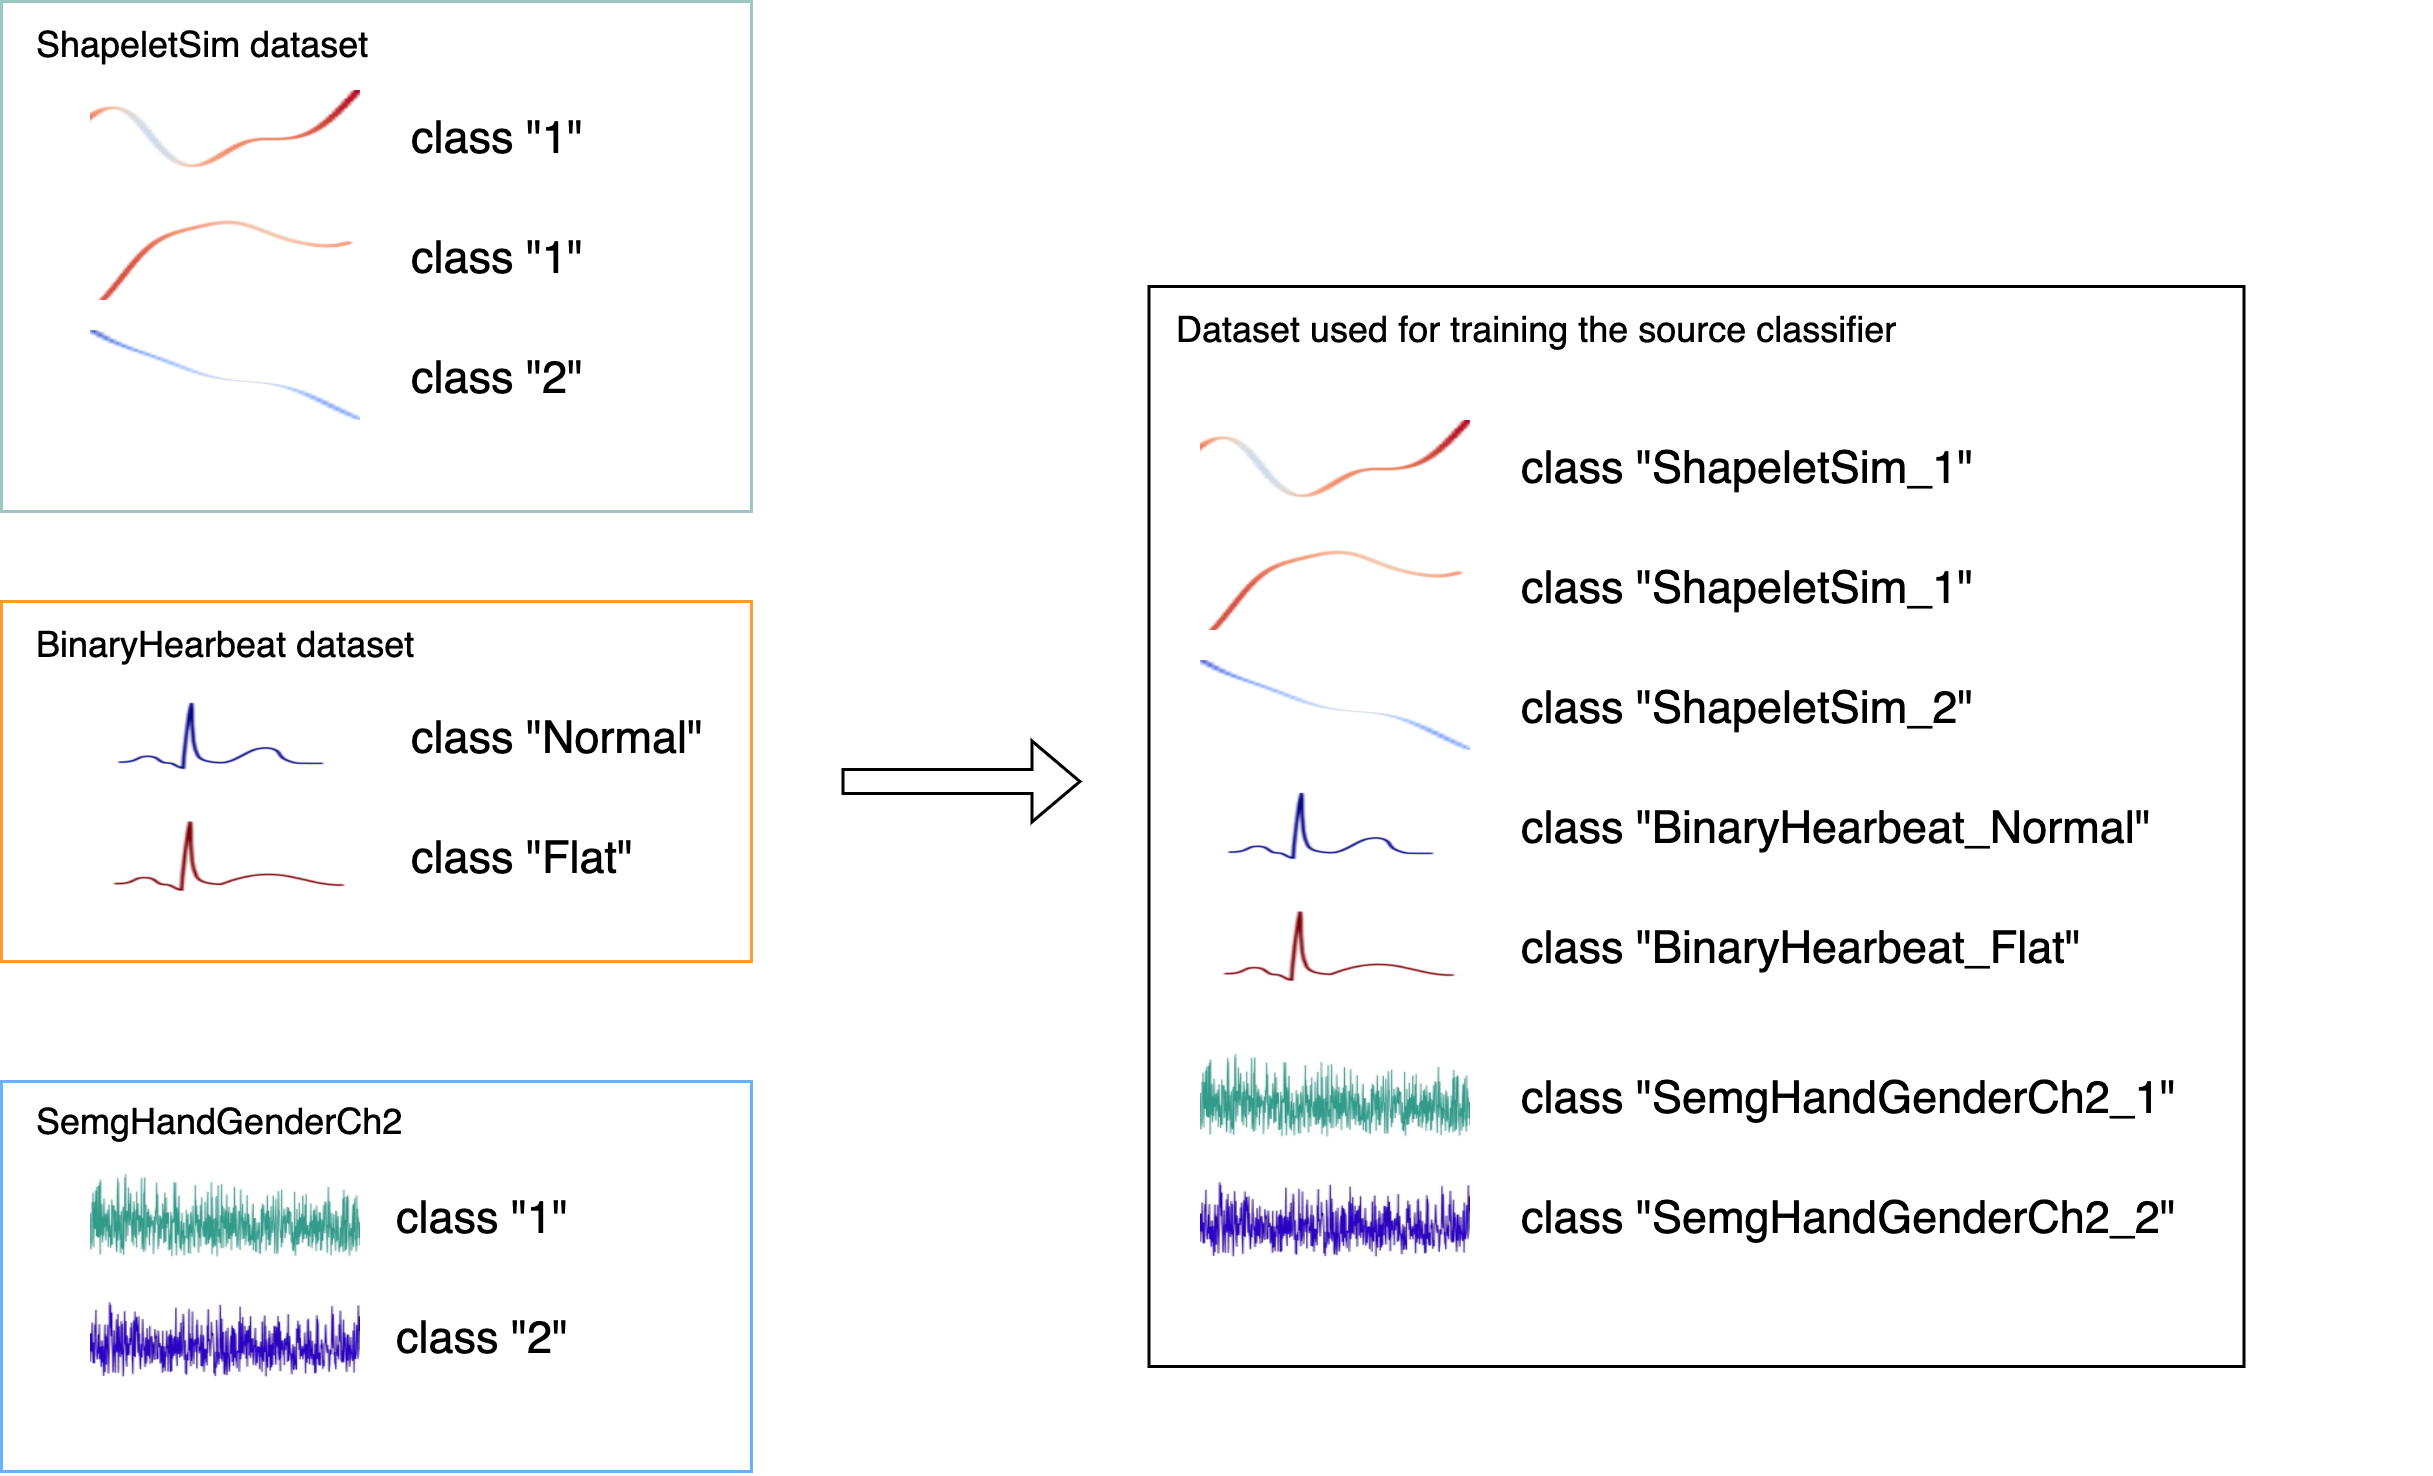
\includegraphics[width=17cm]{imgs/baseline.drawio.png}
\caption{Illustration of preparing the data for the source classifier in the \textit{ baseline} approach.}
\label{fig:baseline_dataset}
\end{figure}

\FloatBarrier
The data batches fed to the model are processed as described in the previous chapter, including length unification within the batch, normalization, and random augmentation of 30\% of the observations.

We obtain a neural network model after training the classifier on the artificial, concatenated dataset. The network (specifically the weights) is then used as a starting point to train on the target dataset. The target classifier is created by removing the last layer, which outputs the probabilities for each class. The layer is replaced by a new layer with randomly initialized weights and output size equal to the number of classes in the last layer. The whole network is then retrained on the target dataset. All weights are updated in the training procedure (freezing the weights is not used).

We compare the results by predicting the classes on the test split of the target dataset. The metrics used for comparison are explained in detail in the Results chapter. We compare the metrics to results obtained by training a network of the same architecture but without transfer learning (with random weights).

\section{Ensemble approach}\label{section:ensemble}
The second approach proposed in this thesis is inspired by the success of ensemble models (e.g.~HIVE-COTE) %TODO more ensemble classifiers
 in time series classification. Small dataset sizes common in time series classification tend to increase the variance error of the classifiers. Therefore the ensemble method is often proposed to decrease the variance and increase the accuracy of predictions. This intuition resembles this approach.

The previous study on transfer learning with a single source dataset \cite{transfer_learning_time_series} showed that though transfer learning generally increases the accuracy, the accuracy was decreased for many experiments. If a dataset differed significantly from the target dataset, a classifier pre-trained on such dataset would not adapt to the target dataset, thus decreasing the accuracy. The same situation is probable with multi-source transfer learning if some datasets are unsuitable for the particular target dataset. In order to mitigate the negative contribution, the ensemble method is used.

Let us assume that we want to perform transfer learning given $N$ source datasets $(X^\mathcal{S}_1, y^\mathcal{S}_1), \dots, (X^\mathcal{S}_N, y^\mathcal{S}_N)$ and a target dataset $(X^\mathcal{T}, y^\mathcal{T})$.
The model is created from $N$ source models. Model $M_i$ is a classifier (e.g.,~a Fully Convolutional Network) trained on the dataset $(X^\mathcal{S}_i, y^\mathcal{S}_i)$. The hyperparameters used for experiments are described in section \ref{section:hyperparameters} and do not differ from those used for the \textit{baseline approach}. % TODO section hyperparameters

Let's recall the notion from the section \ref{mlp_section_related} that a model $M_i$ is a composition of layers, $$M_i(X; \theta_1^i,\dots , \theta_M^i, \beta_1^i,\dots , \beta_M^i) = L_M^i(\dots L_2(L_1(X;\theta_1^i, \beta_1^i);\theta_2^i, \beta_2^i);\theta_M^i, \beta_M^i)$$
To shorten the notation, let us group the first layers together:
$$E(X;\Theta^i, B^i) = L_{M-1}(\dots L_2(L_1(X;\theta_1^i, \beta_1^i);\theta_2^i, \beta_2^i);\theta_{M-1}^i, \beta_{M-1}^i)$$
thus
$$M_i(X; \theta_1^i,\dots , \theta_M^i, \beta_1^i,\dots , \beta_M^i) =  L_M^i(E(X; \Theta^i, B^i);\theta_M^i, \beta_M^i)$$
We assume that the architecture of subsequent layers, except for the last one, is the same for all models $M_i$, $i=1, \dots, N$. Therefore only the last layer has the superscript $\ ^i$. The last layer output size is equal to the number of classes in dataset $i$, which may differ for every model. We also assume that the first layers architecture is the same for all models. Models agnostic to the input size (like FCNs) are advantageous here, as their architecture does not depend on the input size. As for other models, we assume a fixed size of the input data achieved by preprocessing the input data.
The weights $\theta^i_k$ and biases $\beta^i_k$ are obtained from training on dataset $i$.
The target model $M$ is created as follows:
$$M(X) = \frac{1}{N} \sum_{i=1}^N \hat L_M( E(X; \Theta^i, B^i);\hat\theta_M^i, \hat\beta_M^i )$$
The weights $\theta_1^i, \dots, \theta_{M-1}^i$ and biases $\beta_1^i, \dots, \beta_{M-1}^i$ are obtained from training the source models. The last layer $\hat L_M$ is "new", meaning the weights are randomly initialized. The new corresponding weights $\hat\theta_M^i$ and biases $\hat\beta_M^i$ have proper dimensionality (corresponding to the number of classes in the target dataset). This model is then retrained on the target dataset. All weights are updated in the training procedure (freezing the weights is not used).

A graphical example of the process can be found in Figure \ref{fig:ensemble_architecture}.


\FloatBarrier
\begin{figure}[h!]
\centering
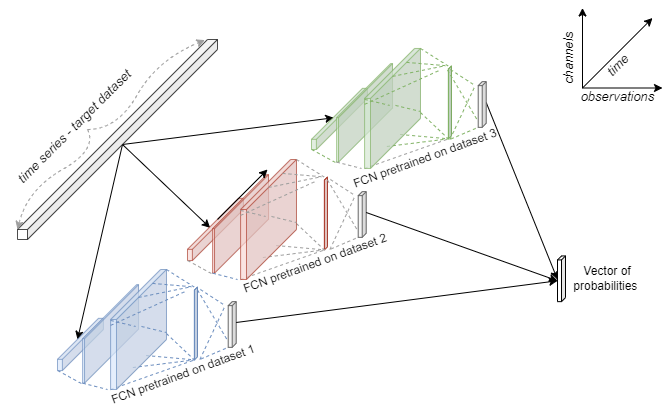
\includegraphics[width=17cm]{imgs/ensemble_architecture.png}
\caption{Illustration of the\textit{ ensemble }approach based on $N=3$ source models (Fully convolutional networks in this case). If a layer is colored, it means that the weights in this layer are initialized by pre-training on one of the source datasets. The last layer in each model is new.}
\label{fig:ensemble_architecture}
\end{figure}

\FloatBarrier


\section{Selecting the source datasets for multi-source transfer learning}\label{section:selecting}
In both multi-source learning approaches described above (\textit{baseline} and \textit{ensemble} approaches), we do not impose any restrictions on the source datasets themselves. Neither of the two approaches does not include any rules on how the source datasets correspond to the target dataset. In the experiments conducted in this thesis, two approaches for picking the datasets are proposed. In the first approach, we randomly choose $N$ datasets from a given category corresponding to the target dataset. To illustrate, let us say that the objective is to train a target classifier on the \texttt{InlineSkate} dataset, which belongs to the \texttt{Motion} category in the UCR archive. Then the source datasets are picked randomly from the given category, which could be \texttt{UWaveGestureLibraryX, AsphaltPavementType, ToeSegmentation2, CricketZ, UWaveGestureLibraryZ}.


The second approach described was based on a similarity measure. The inter-dataset similarity measure called DTW barycenter averaging was described in \ref{DTW_choosing}. The intuition behind the second approach is that usually transfer learning benefits if the domains are similar. In order to measure the similarity between datasets, the DBA distances were computed for all pairs of datasets in a given category. Then, for a given target dataset, $N$ datasets minimalizing the distance to the target dataset were used for pretraining the source network (either in \textit{baseline} or \textit{ensemble} approach). The dataset still belonged to the same UCR category as the target dataset.
\section{Environment and code structure}
The solution is written in Python 3.8, mainly utilizing the library \texttt{Keras} from the \texttt{TensorFlow} library. The structure of the code is as follows:

\begin{verbatim}
./MASTER-THESIS/SRC
+---data
|   ...
+---experiments
|   +---no_transfer_learning
|   +---transfer_learning
+---mlflow_logging
+---models
+---preprocessing
+---reading
+---results
|   +---baseline
|   +---baseline_vs_ensemble
|   +---dba_vs_random
|   +---ensemble
|   +---ensemble_dba_3_vs_5
|   +---ensemble_dba_5_vs_8
+---selecting
\end{verbatim}

The folders contain the following content:
\begin{itemize}
\item \texttt{data} - \texttt{ts} and \texttt{arff} files downloaded from the UCR archive,   serialized \texttt{keras} models to use in the ensemble (see section  \ref{section:ensemble}) and \texttt{numpy} files containing all series from UCR archive concatenated to one dataframe (see section \ref{section:reading})
\item \texttt{experiments}  experiments corresponding to scenarios described in \ref{section:ensemble} and section \ref{section:baseline} and without the use of transfer learning for comparison purposes.
\item \texttt{mlflow\_logging} - utility functions to write metrics and parameters of the experiments and runs to MlFlow
\item \texttt{models} - model architecture definitions in \texttt{keras} syntax
\item \texttt{preprocessing} - utility functions for preprocessing purposes, definitions of DataGenerators (see \ref{section:preprocessing}.
\item \texttt{reading} - script for reading \texttt{ts} and \texttt{arff} files, creating the concatenated dataset (see \ref{section:reading})
\item \texttt{results} - scripts for preparing results (as plots or sole values) of comparing experiments conducted by scripts in the \texttt{experiments} directory. The experiments are further described in \ref{section:ensemble} and section \ref{section:baseline}. The results are described in chapter \ref{chapter:results}
\item \texttt{selecting} - source dataset selection methods (see \ref{section:selecting})

\end{itemize}

The model training experiments were run in Google Colab with GPU. Other scripts, for example, to calculate DBA similarity measures or to summarize results gathered in MlFlow were run locally.
\chapter{Results}\label{chapter:results}
The results and metrics of classifiers obtained from training networks with transfer learning were compared to the results obtained without transfer learning. The performance of the target classifier in the\textit{ ensemble }approach was compared to an ensemble model with the same amount of component models in the ensemble.

\section{Experiments}
Each experiment recorded in MlFlow corresponds to one training setting. An example setting may be, e.g.~\begin{itemize}
\item training a network using the \textit{ensemble approach}, with 5 datasets picked using the DBA similarity measure
 \item training a network using the \textit{baseline approach}, with 5 source datasets picked randomly
 \item training an ensemble of FCNs without transfer learning

\end{itemize}
Following the MlFlow convention, each experiment consisted of several runs, each corresponding to one target dataset from the category \texttt{MOTION} and \texttt{IMAGE}. This is shown on screenshot \ref{fig:mlflow_screnshot}. When comparing averaged results, then the result was averaged on all runs (61 runs for each experiment).


\FloatBarrier

\begin{figure}[h!t]
\centering
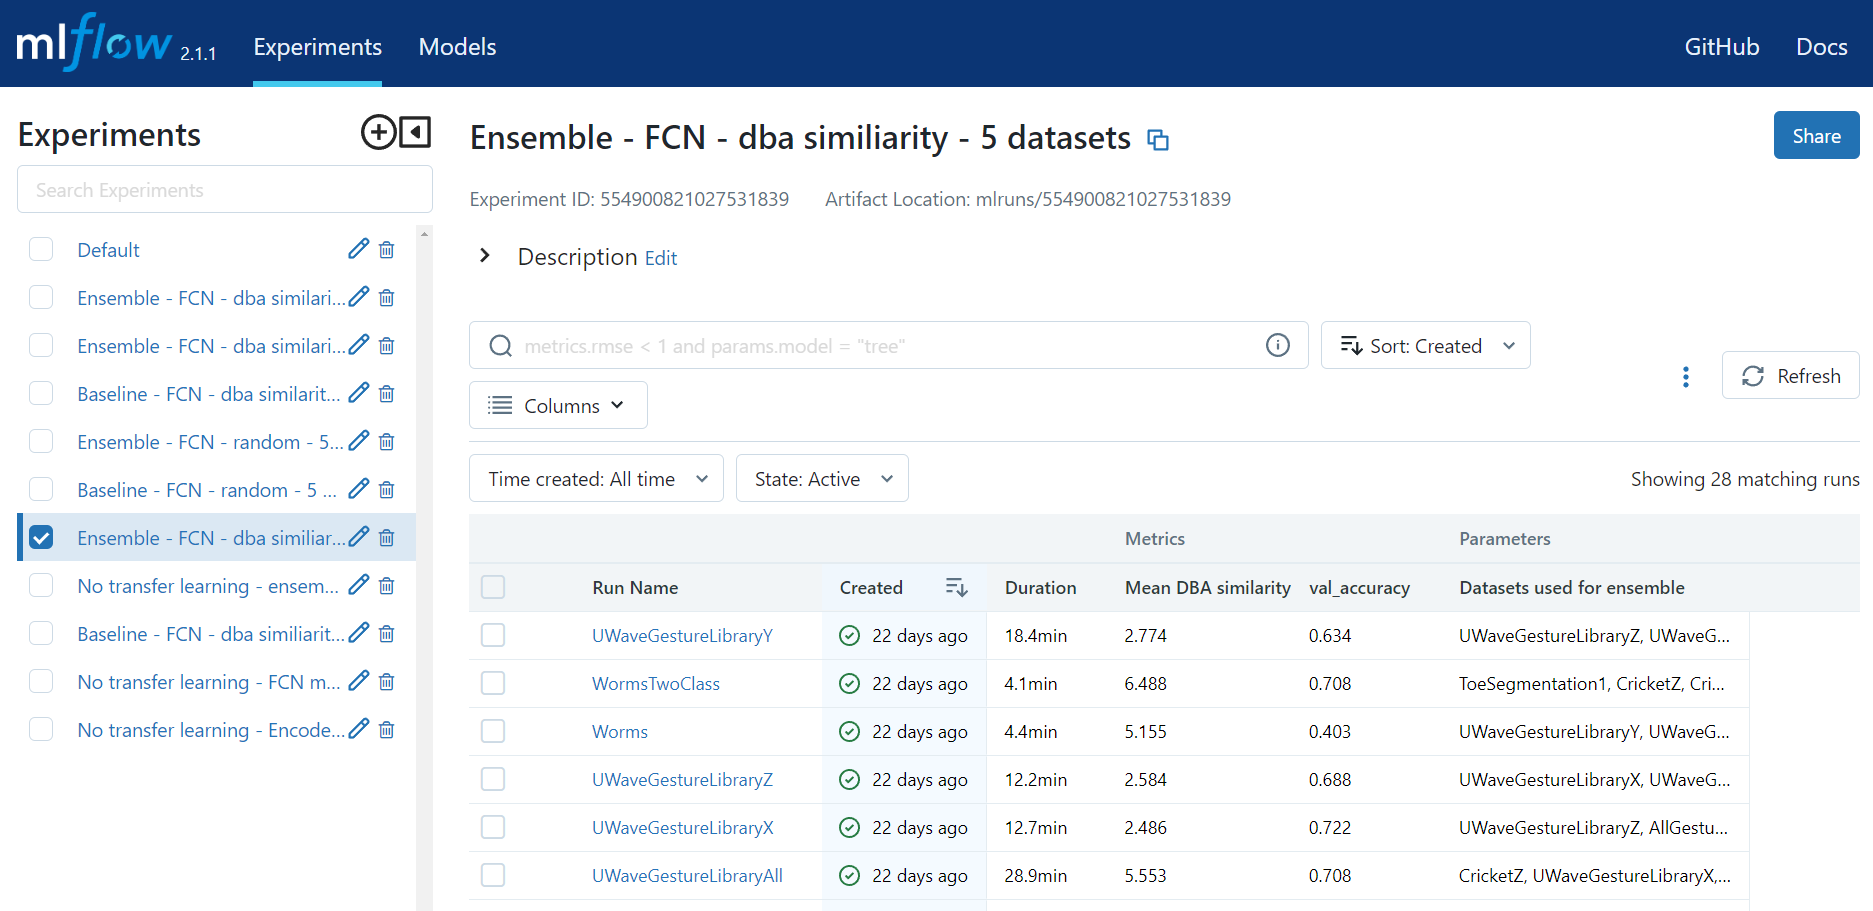
\includegraphics[width=17cm]{imgs/mlflow_screenshot.png}
\caption{The structure of experiments recorded in MlFlow. Each experiment corresponds to a different setting, and each run corresponds to a model trained on a different target dataset (and consequently different source datasets).}
\label{fig:mlflow_screnshot}
\end{figure}
\FloatBarrier
\section{Evaluation of the \textit{baseline} approach}
The \textit{baseline} approach, in which a single Fully Convolutional Network was pre-trained and fine-tuned, was compared to results obtained from training a single FCN model on the target dataset only. For this comparison, we used a Fully Convolutional Network as the model, and five source datasets were selected to minimize the DBA distance to the target dataset. Figure \ref{fig:baseline_acc} shows the accuracy and loss in each epoch, averaged over all experiments conducted.


\FloatBarrier

\begin{figure}[h!t]
\centering
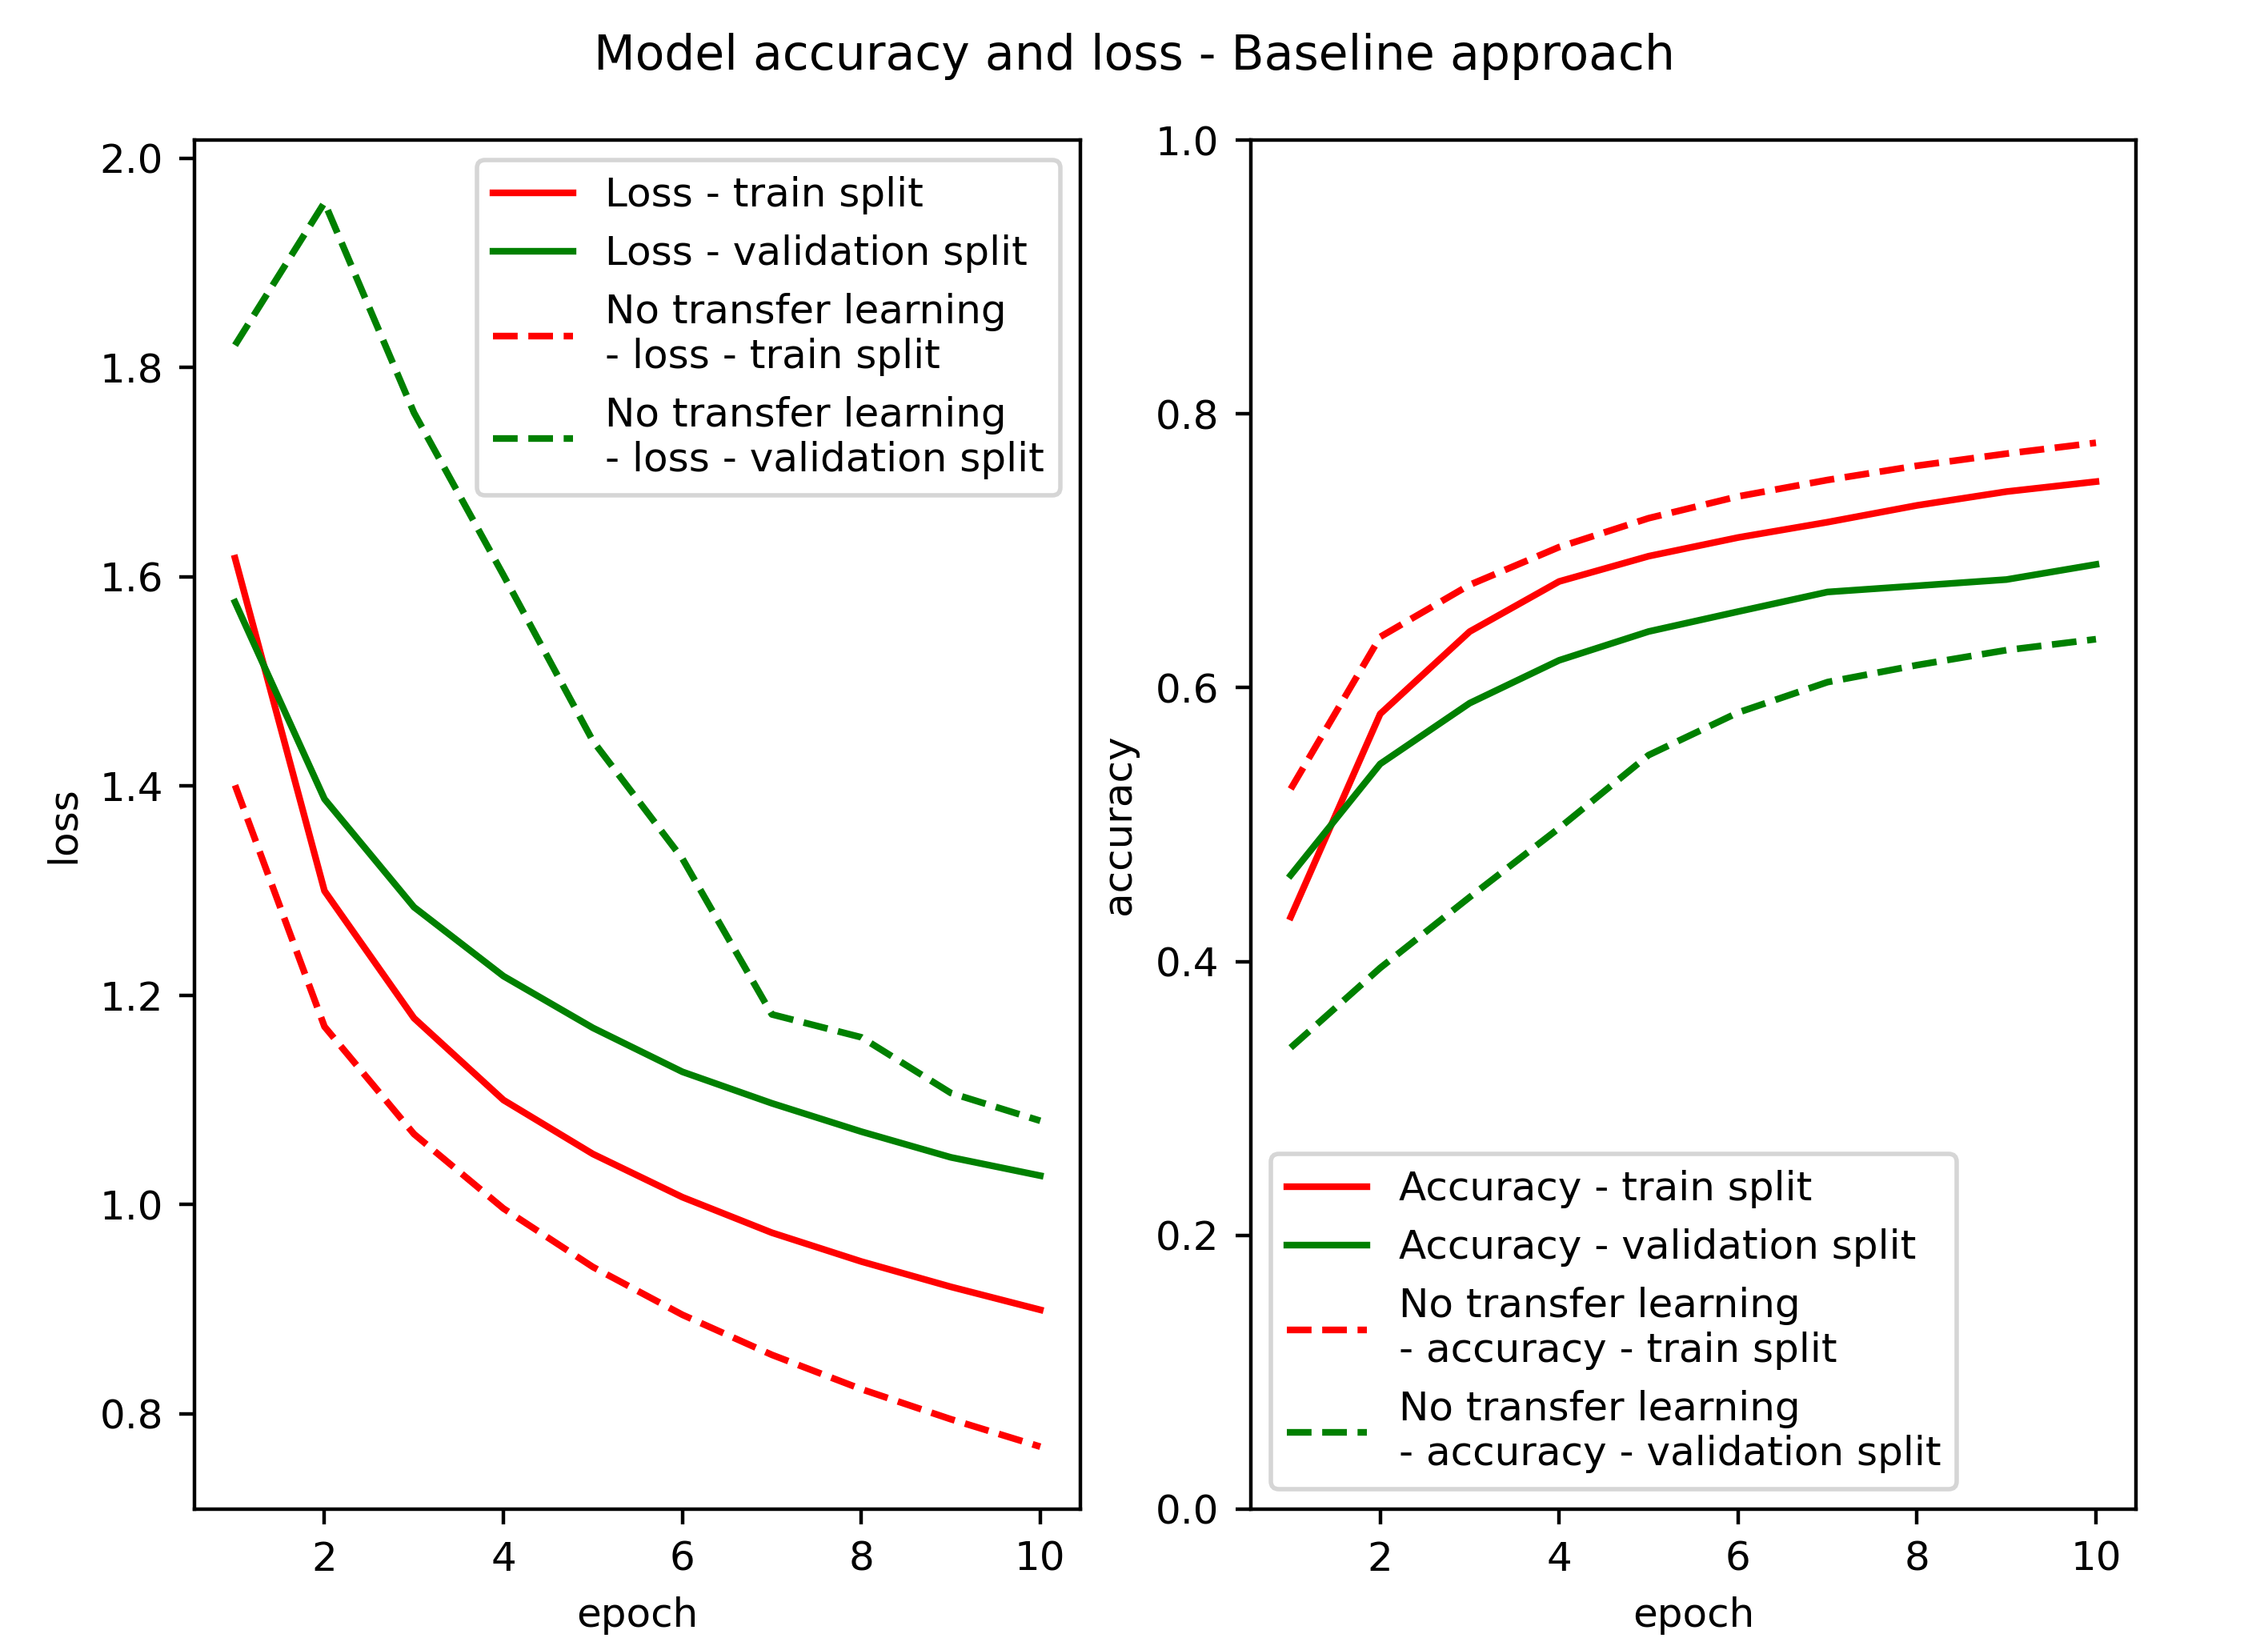
\includegraphics[width=17 cm]{imgs/baseline/loss_acc.png}
\caption{Averaged accuracy and loss obtained from transfer learning with the \textit{baseline} approach, compared to a single FCN trained only on the target dataset.}
\label{fig:baseline_acc}
\end{figure}
\FloatBarrier
The most remarkable improvement is visible in the first epochs of the training process, which suggest that the network uses the knowledge learned from the previous task. As the training continues, the advantage is less significant. In Figure \ref{fig:win_tie_loss_baseline}, we show a comparison win-tie-loss diagram for the fifth and tenth epochs.
Transfer learning makes the gap between accuracy/loss on the train and validation split smaller. This can mean that the model is less prone to overfitting and hence generalizes better due to exposure to more diverse examples in the pre-training phase.
\FloatBarrier
\begin{figure}[h!t]
\centering
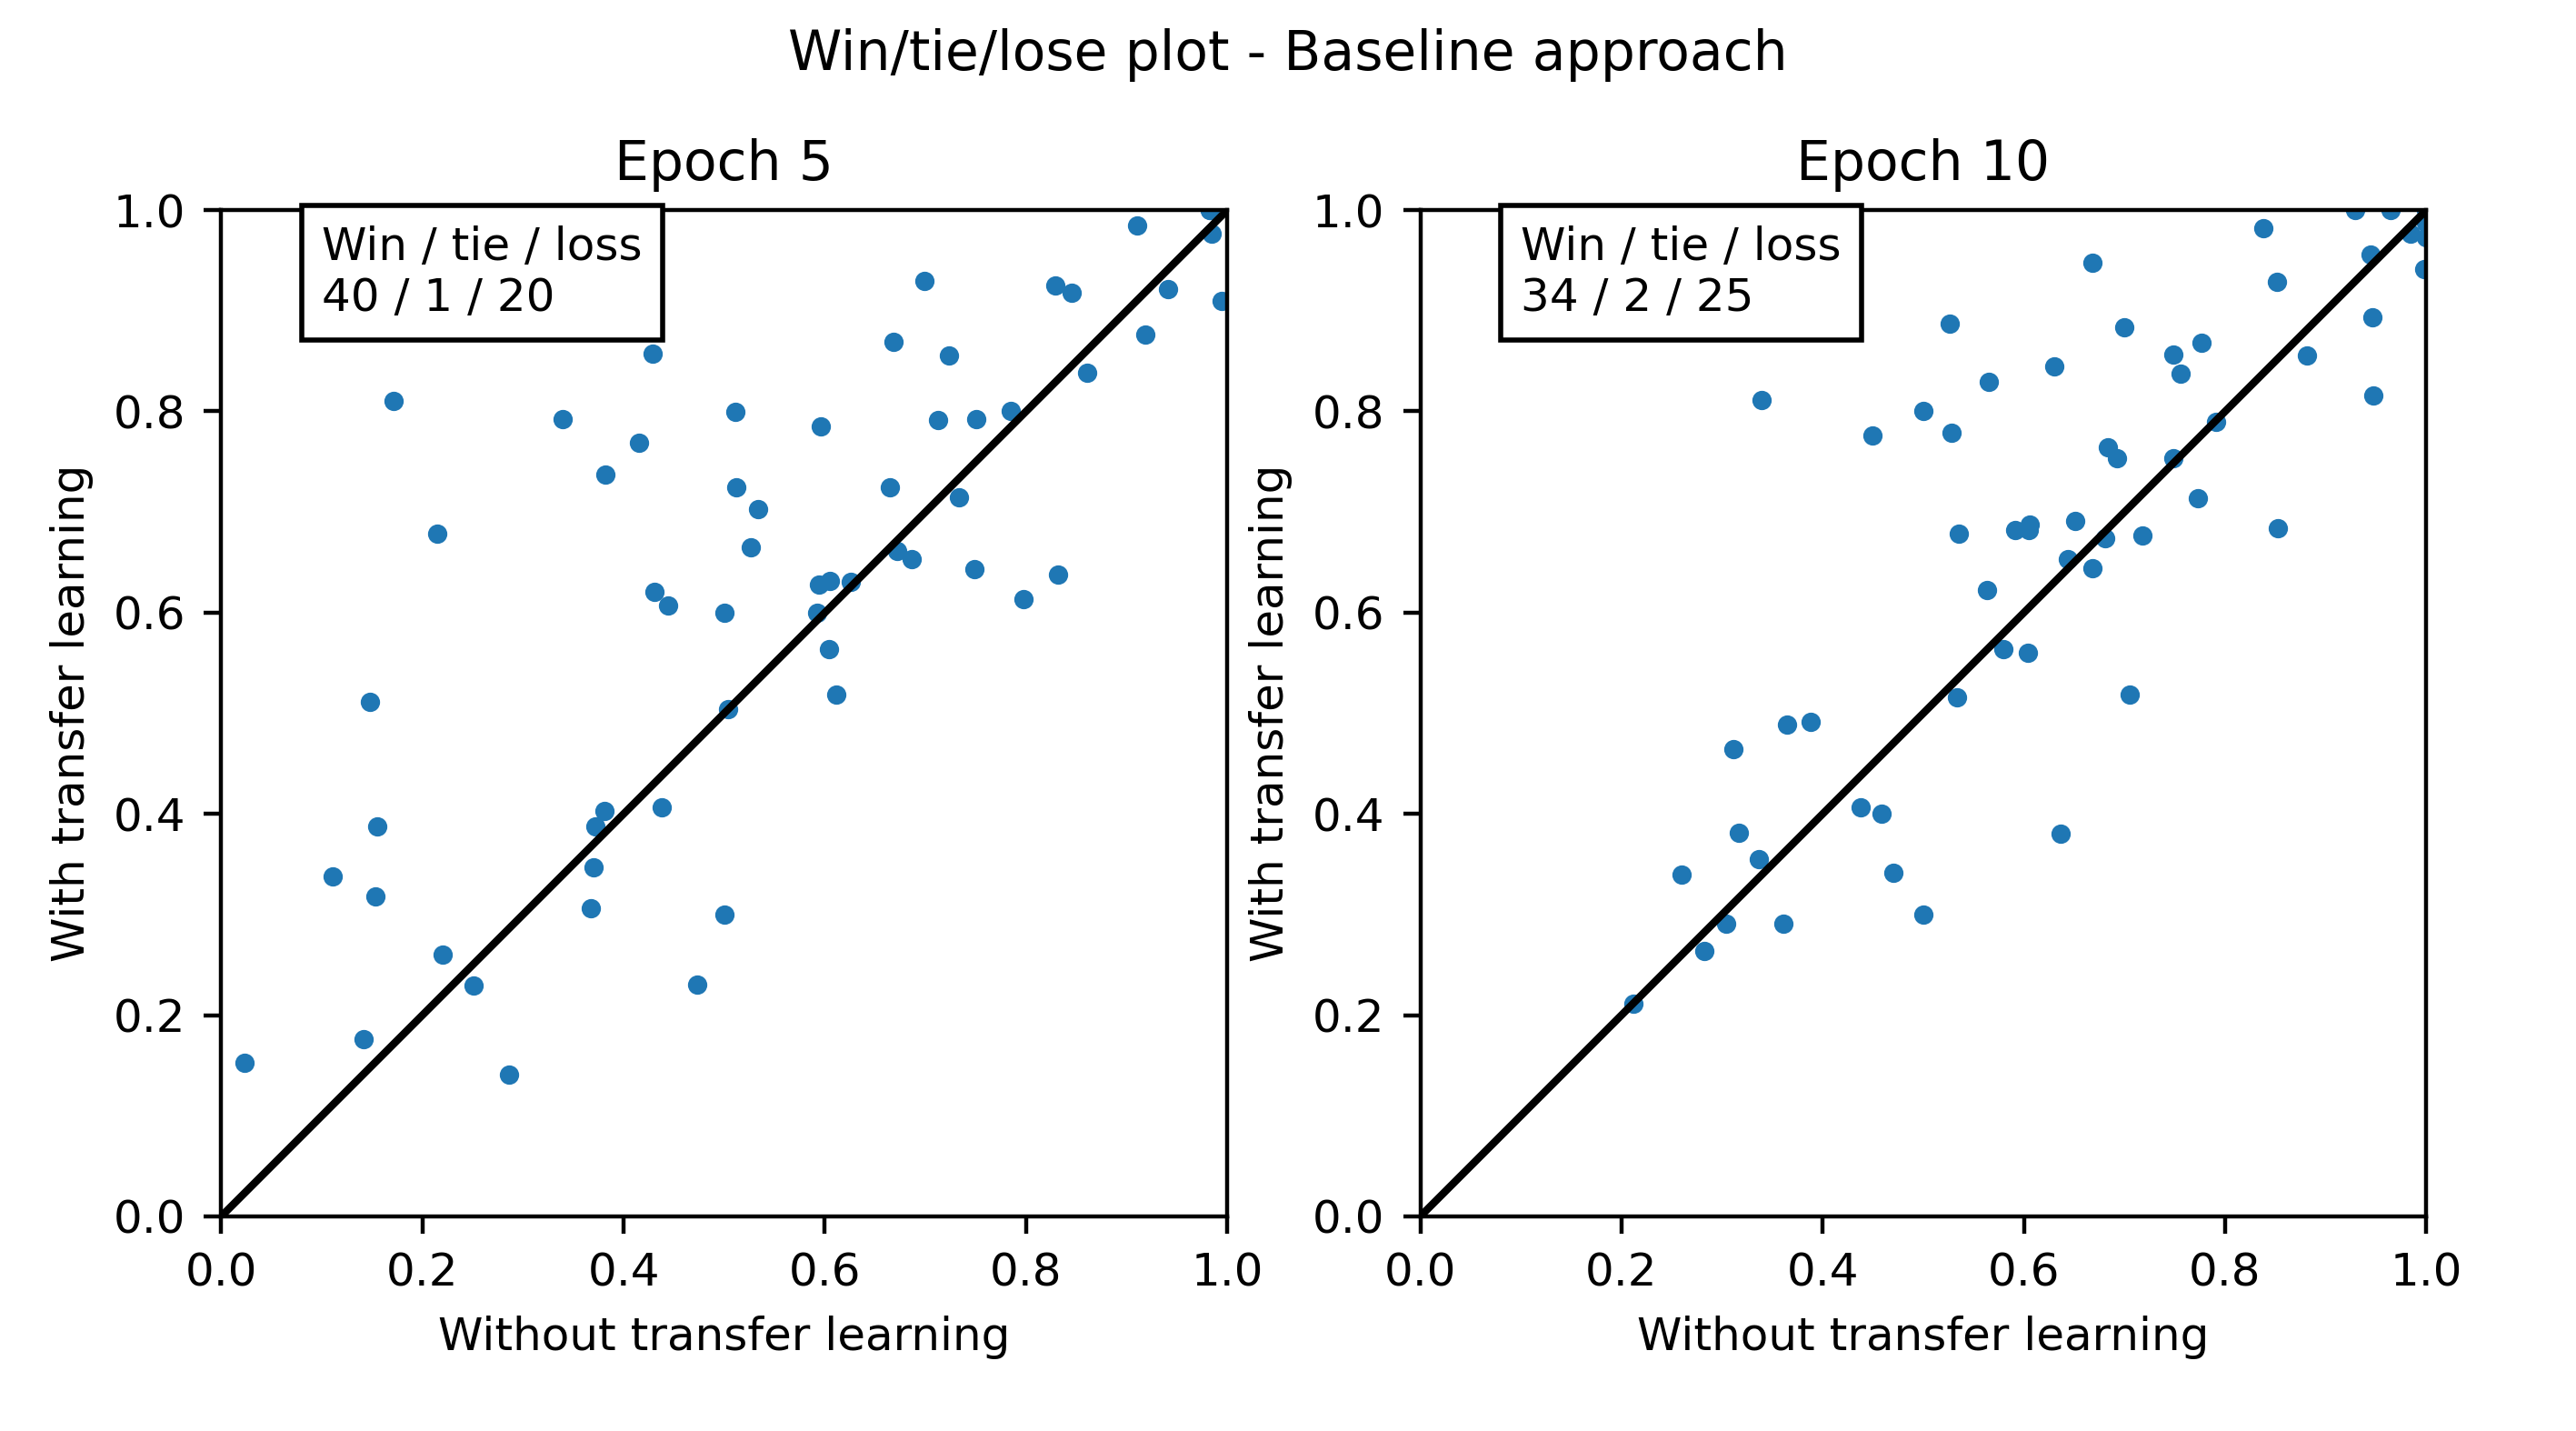
\includegraphics[width=17 cm]{imgs/baseline/win_tie_lose_epoch.png}
\caption{Win-tie-loss plot. This plot shows the validation accuracy in each run's 5th and 10th epoch (corresponding to a target dataset). The y-axis corresponds to the baseline approach, and the x-axis to the approach without transfer learning. If a dot is above the diagonal, then it means that the transfer learning was beneficial.}
\label{fig:win_tie_loss_baseline}
\end{figure}

\FloatBarrier
\section{Evaluation of the \textit{ensemble} approach}
In the \textit{ensemble} approach, we created an ensemble model from 5 FCN models pre-trained on different datasets. The pre-trained ensemble was fine-tuned on the target dataset, and the results were compared to a model whose architecture was identical to the ensemble, but the weights were initialized randomly. Transfer learning improved accuracy and loss, similarly as in the \textit{baseline} approach. Figure \ref{fig:ensemble_acc} shows the comparison of accuracy and loss in each epoch, averaged over all runs (each run corresponds to a target dataset).

\FloatBarrier

\begin{figure}[h!t]
\centering
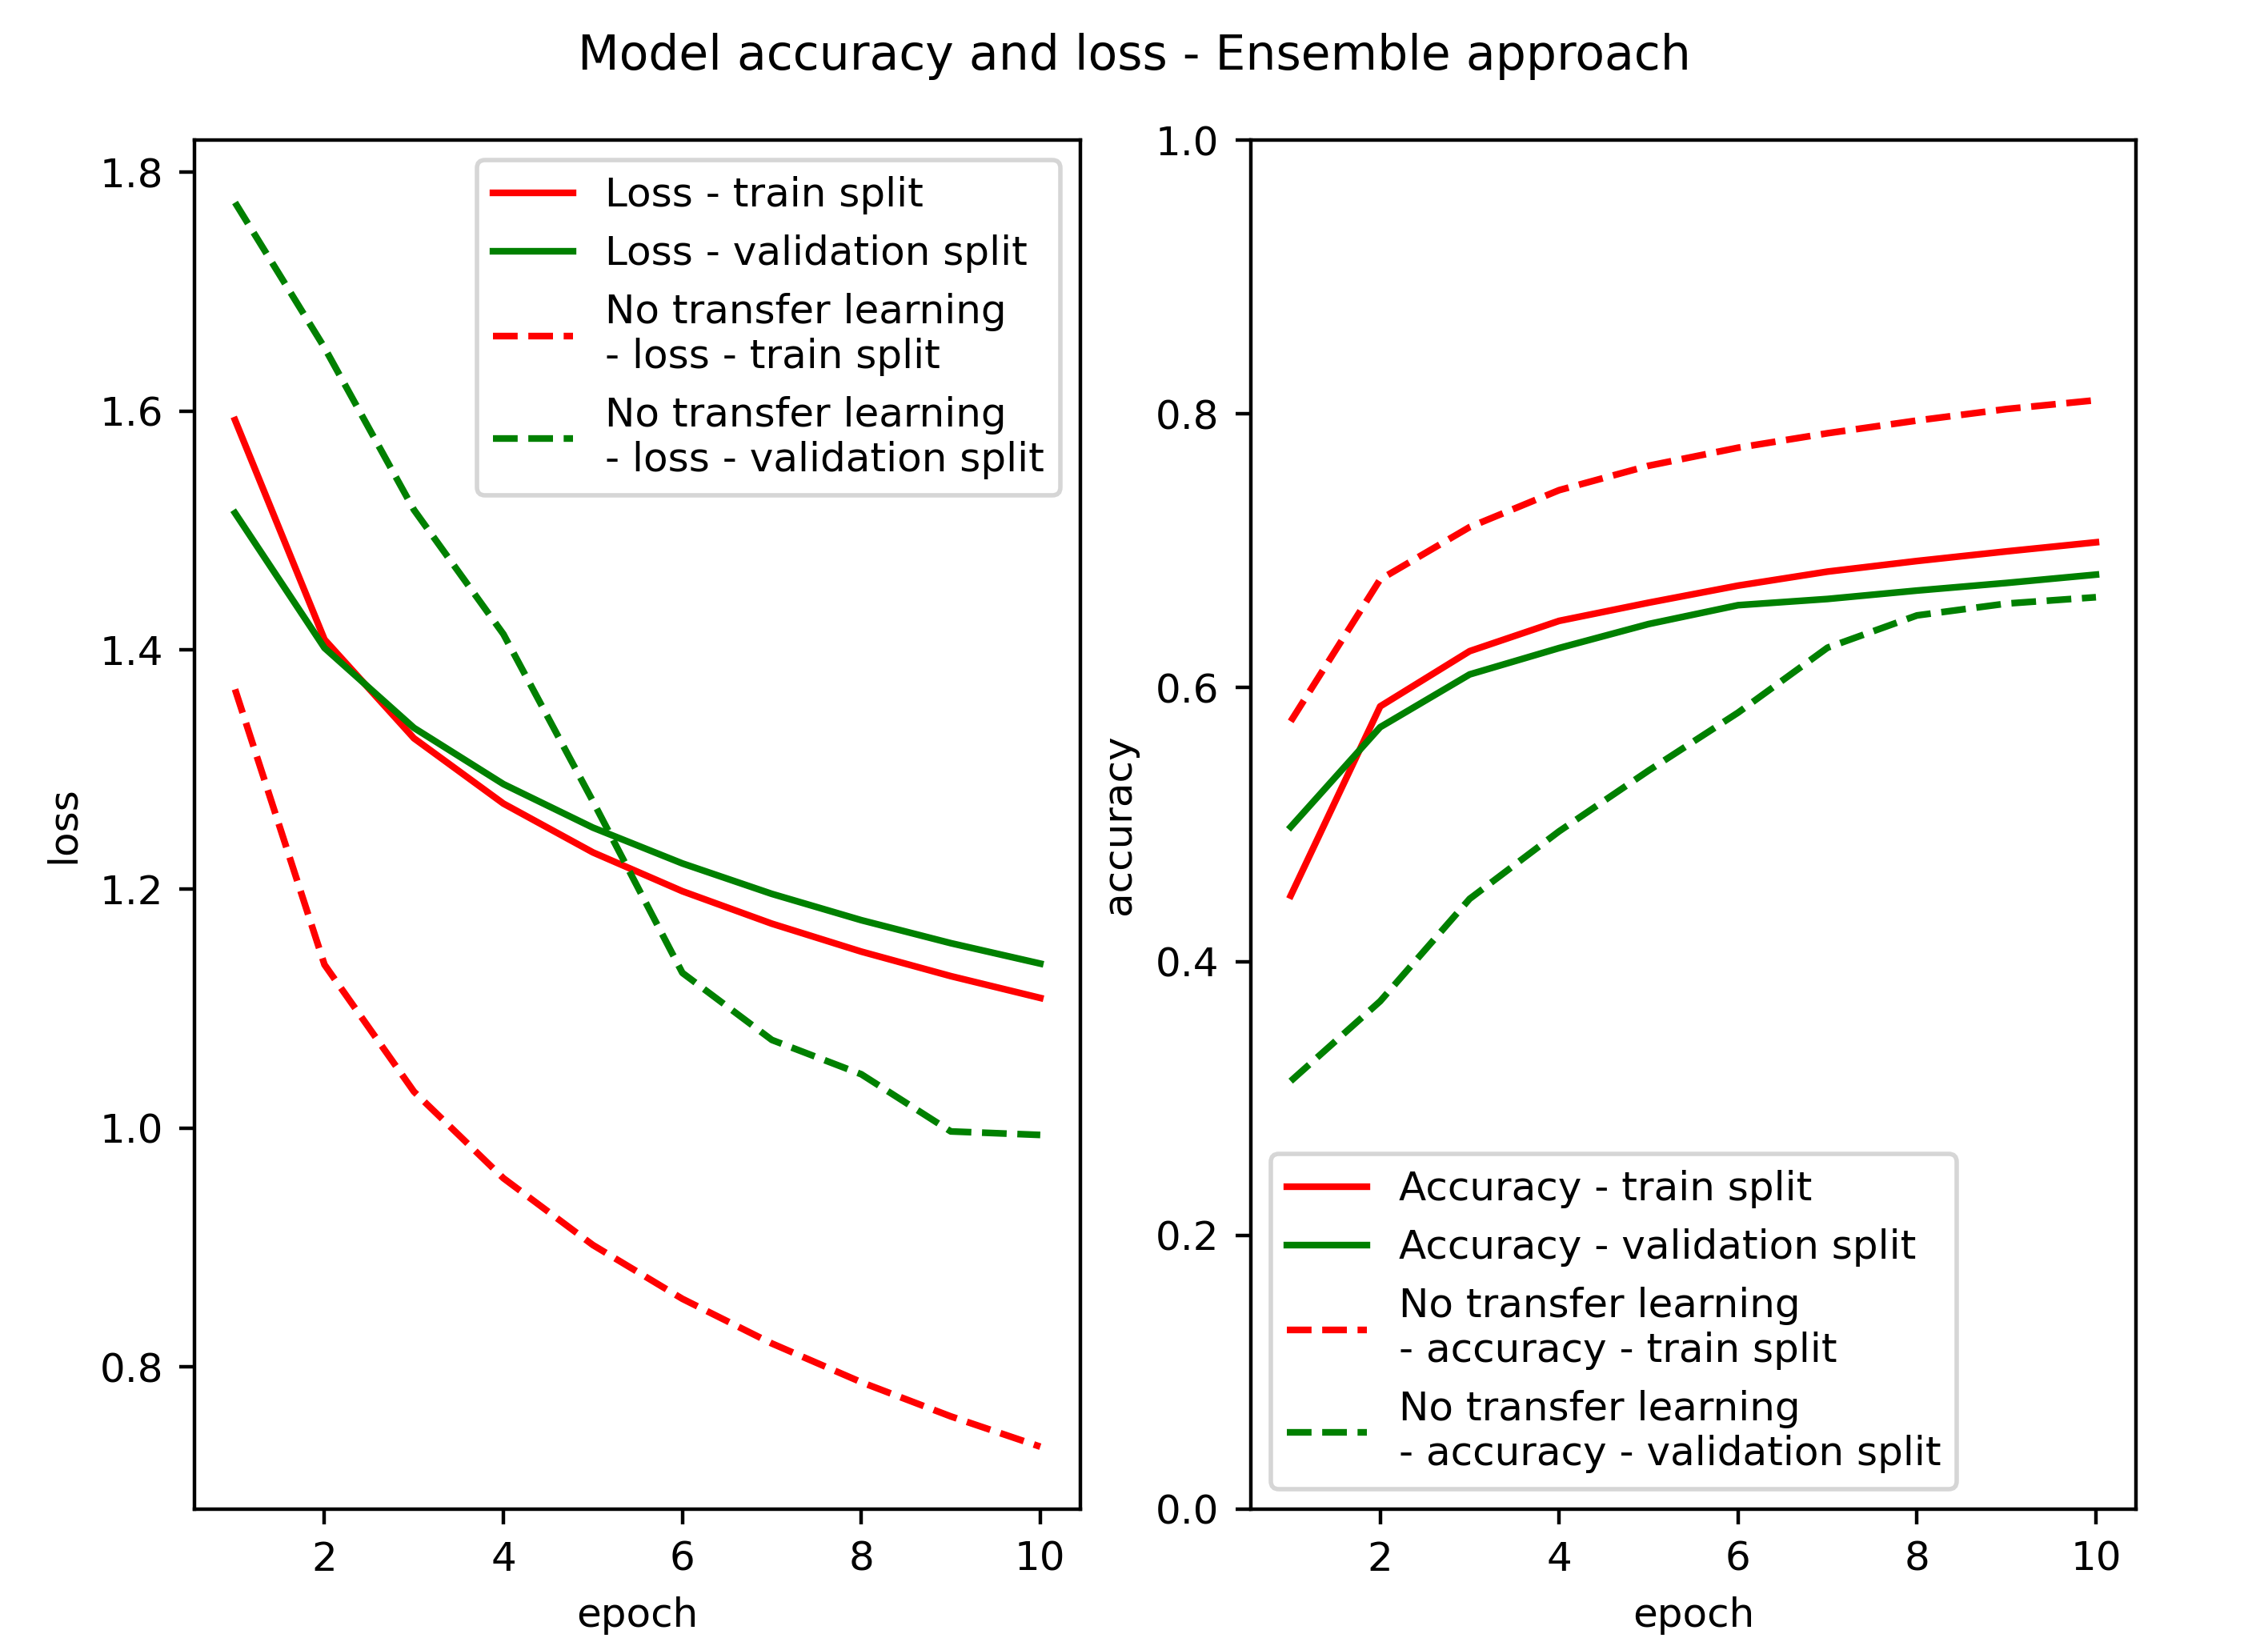
\includegraphics[width=17 cm]{imgs/ensemble/loss_acc.png}
\caption{Averaged accuracy and loss obtained from transfer learning with the \textit{ensemble} approach, compared to an ensemble of FCN models trained only on the target dataset.}
\label{fig:ensemble_acc}
\end{figure}
\FloatBarrier
We also present a win-tie-loss diagram for the \textit{baseline} approach in Figure \ref{fig:win_tie_loss_ensemble}. We see that in the final epoch, most of the datasets did not benefit from transfer learning, but if they did, the benefit was relatively more significant than in the \textit{baseline} approach.

\FloatBarrier
\begin{figure}[h!t]
\centering
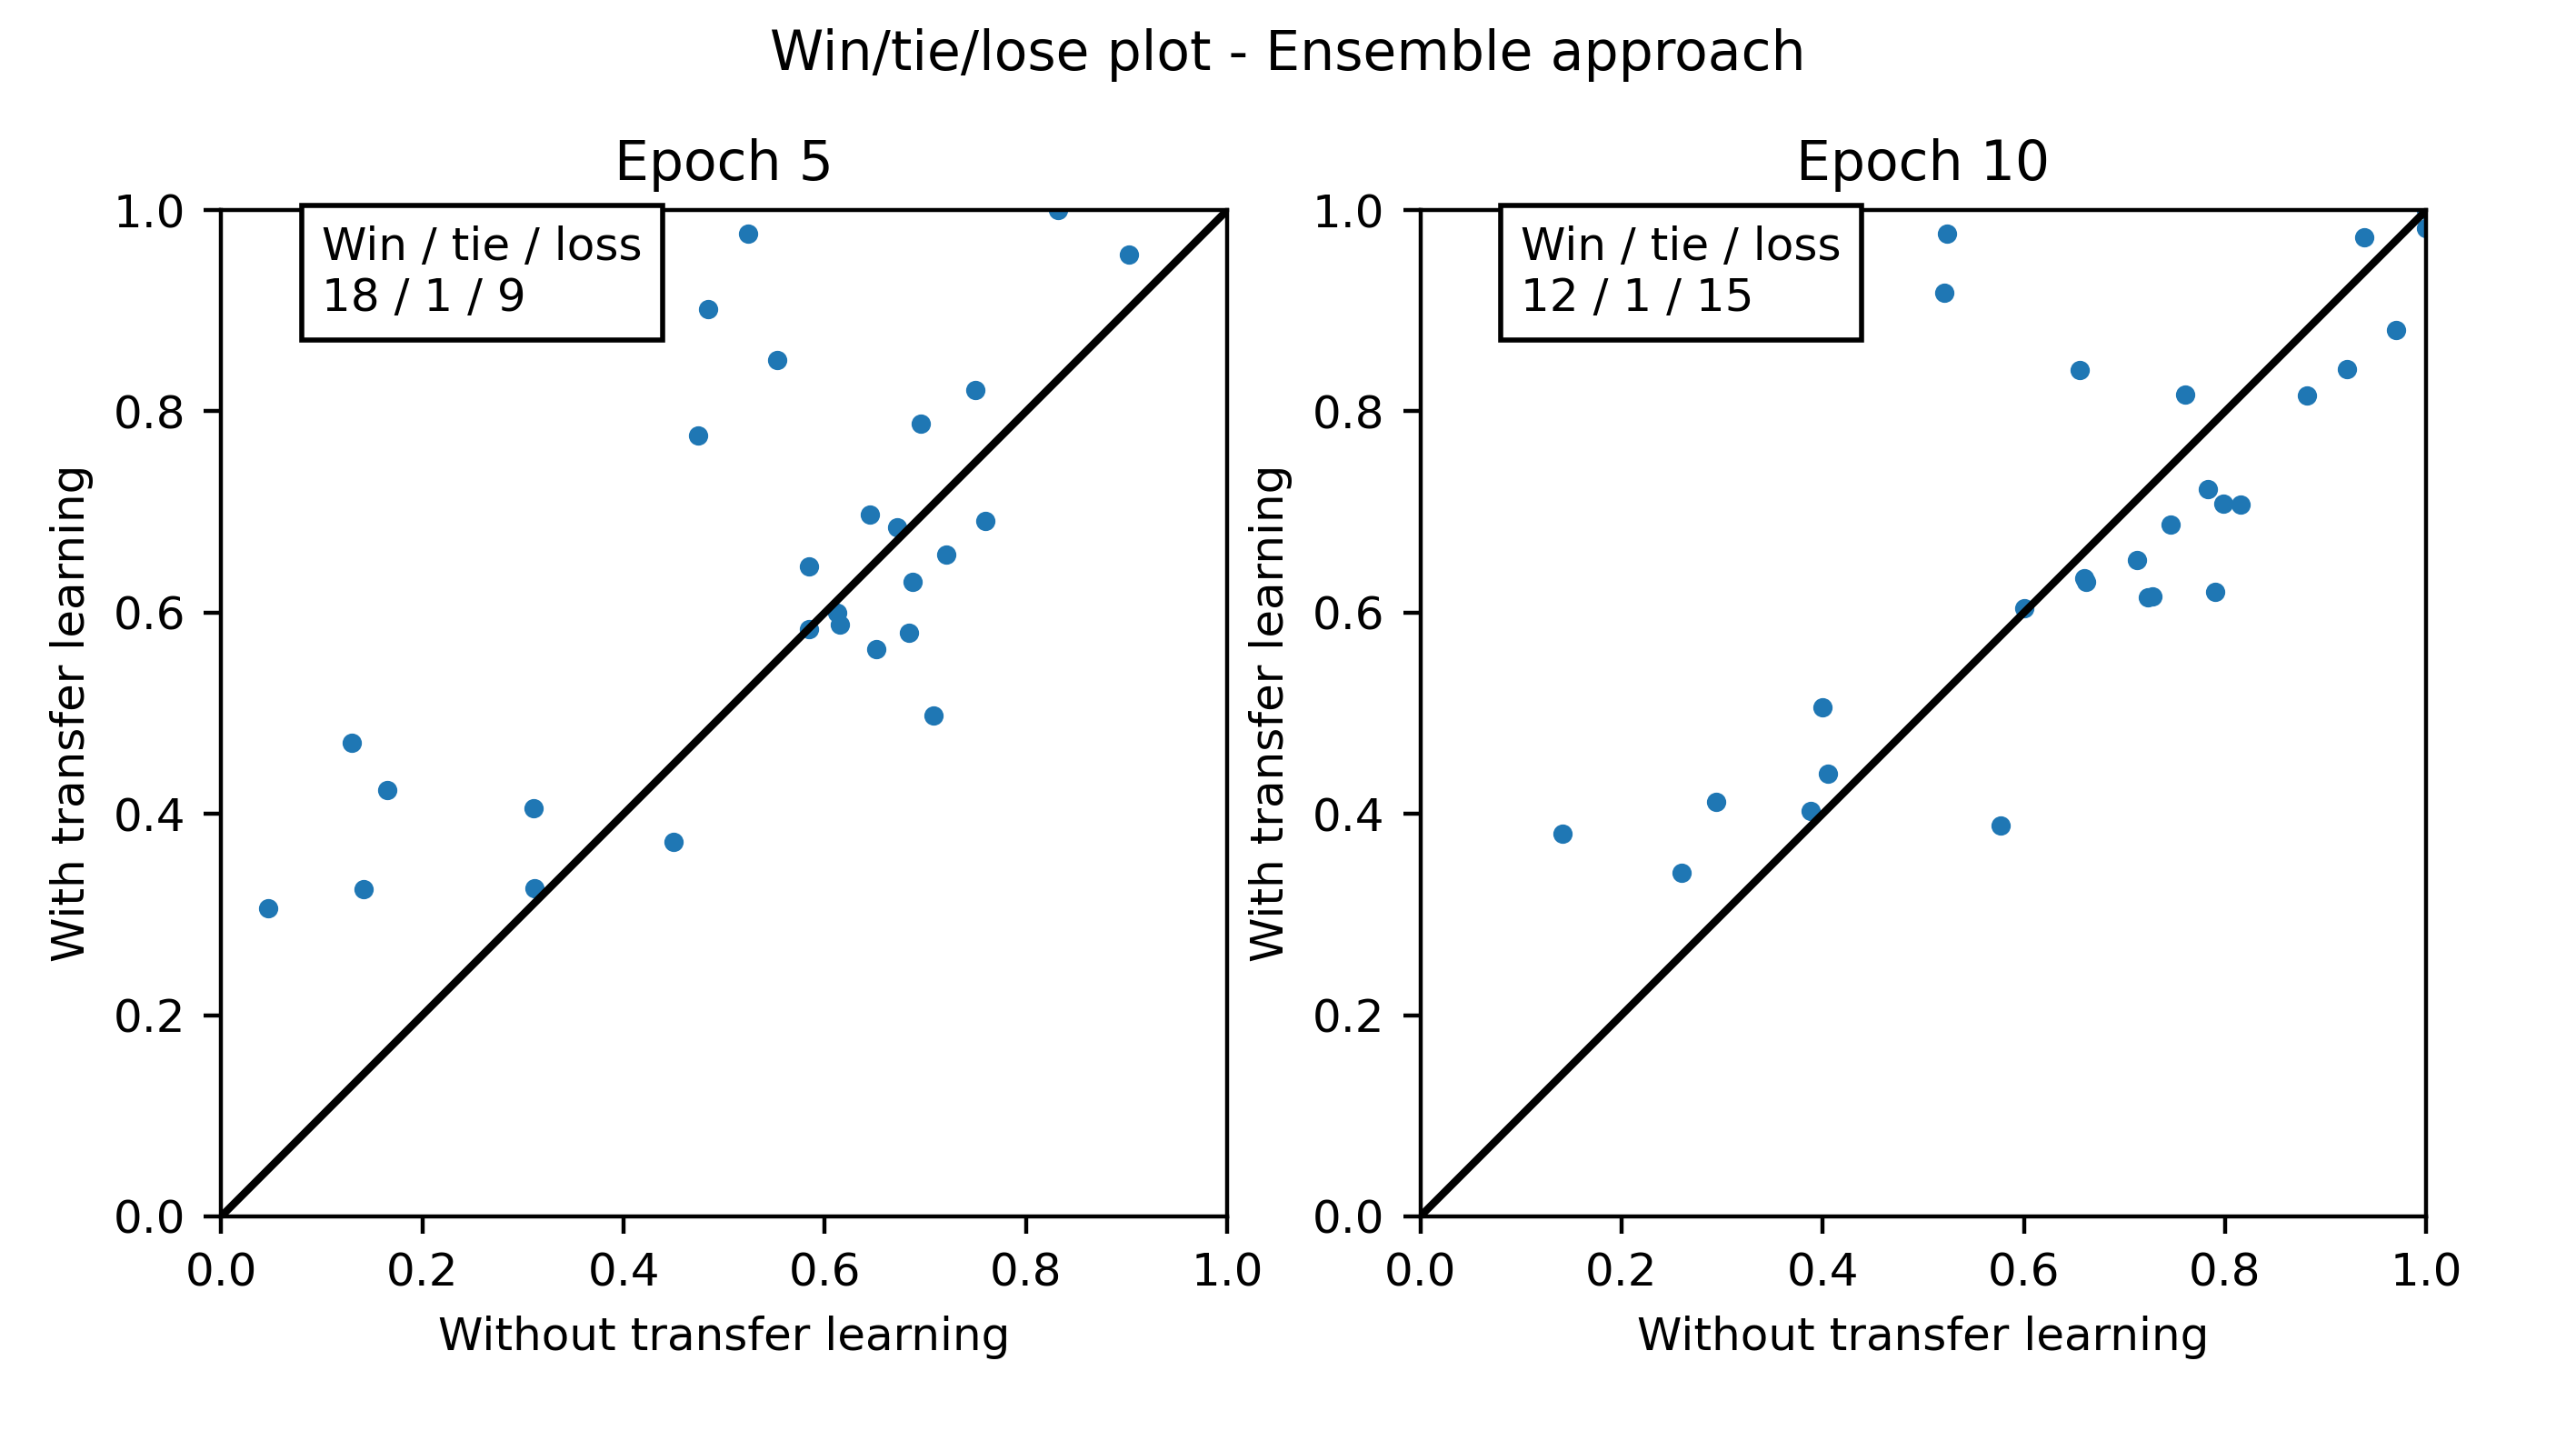
\includegraphics[width=17 cm]{imgs/ensemble/win_tie_lose_epoch.png}
\caption{Win-tie-loss plot. This plot shows the validation accuracy in the 5th and 10th epoch for each run (corresponding to a target dataset). The y-axis corresponds to the \textit{ensemble} approach and the x-axis to the approach without transfer learning. If a dot is above the diagonal, then it means that the transfer learning was beneficial.}
\label{fig:win_tie_loss_ensemble}
\end{figure}
The model used in the ensemble approach consisted of more parameters, thanks to ensembling. This, together with the small sizes of datasets in the UCR archive, might lead to overfitting. As we see in the plot, the gap between accuracy and loss for validation and test split is more significant in the model trained without transfer learning. This may indicate that the models were overfitted. Exposing the models to a larger amount of data in the pre-training phase reduces overfitting. We see that for the transfer learning results, the gap between metrics for validation and train split is smaller. Also, the accuracy of the train split is smaller, which suggests that the overfitting is mitigated.

\section{Comparison of\textit{ baseline }and\textit{ ensemble }approaches}
We see that in both approaches, the results were improved compared to training a network from scratch. Figure \ref{fig:baseline_vs_ensemble} shows the accuracy and loss per each epoch averaged over several runs (corresponding to target datasets)

\FloatBarrier
\begin{figure}[h!t]
\centering
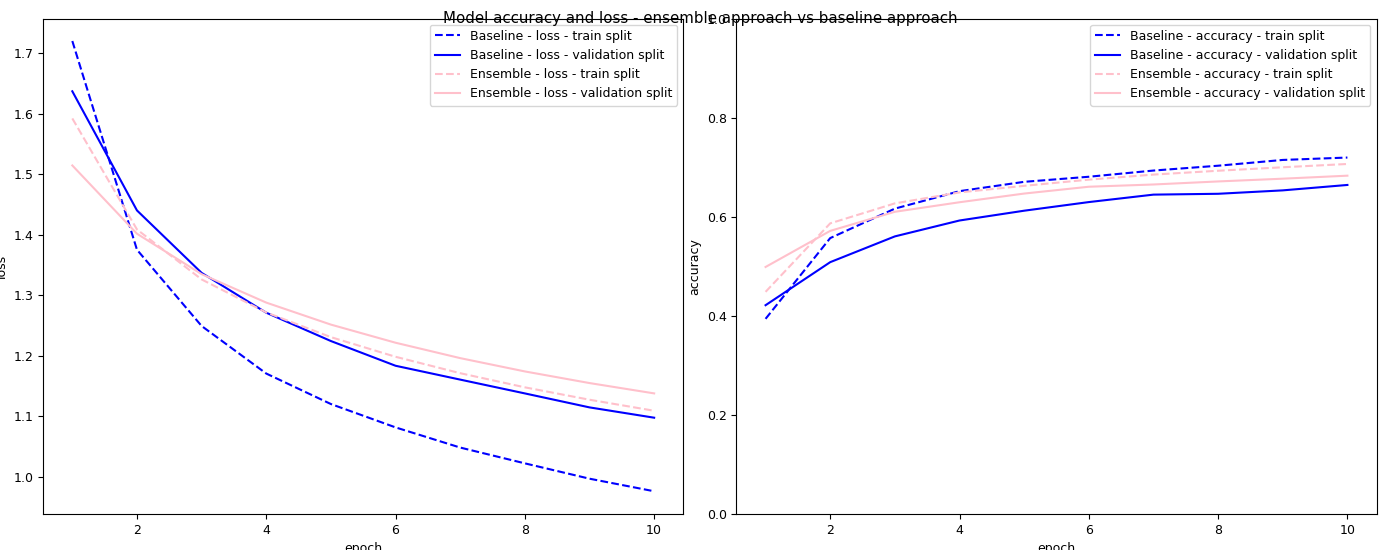
\includegraphics[width=15.5cm]{imgs/baseline_vs_ensemble/loss_acc.png}
\caption{Comparison of loss and accuracy for\textit{ baseline }approach and\textit{ ensemble }approach. }
\label{fig:baseline_vs_ensemble}
\end{figure}
\FloatBarrier
Similarly, as in the two previous sections, where we compared \textit{ensemble} and \textit{baseline} approaches to training without transfer learning, Figure \ref{fig:win_tie_loss_baseline_vs_ensemble} shows a win-tie-loss diagram for 5th and 10th epoch comparing the \textit{baseline} and \textit{ensemble} approaches.

\FloatBarrier
\begin{figure}[h!t]
\centering
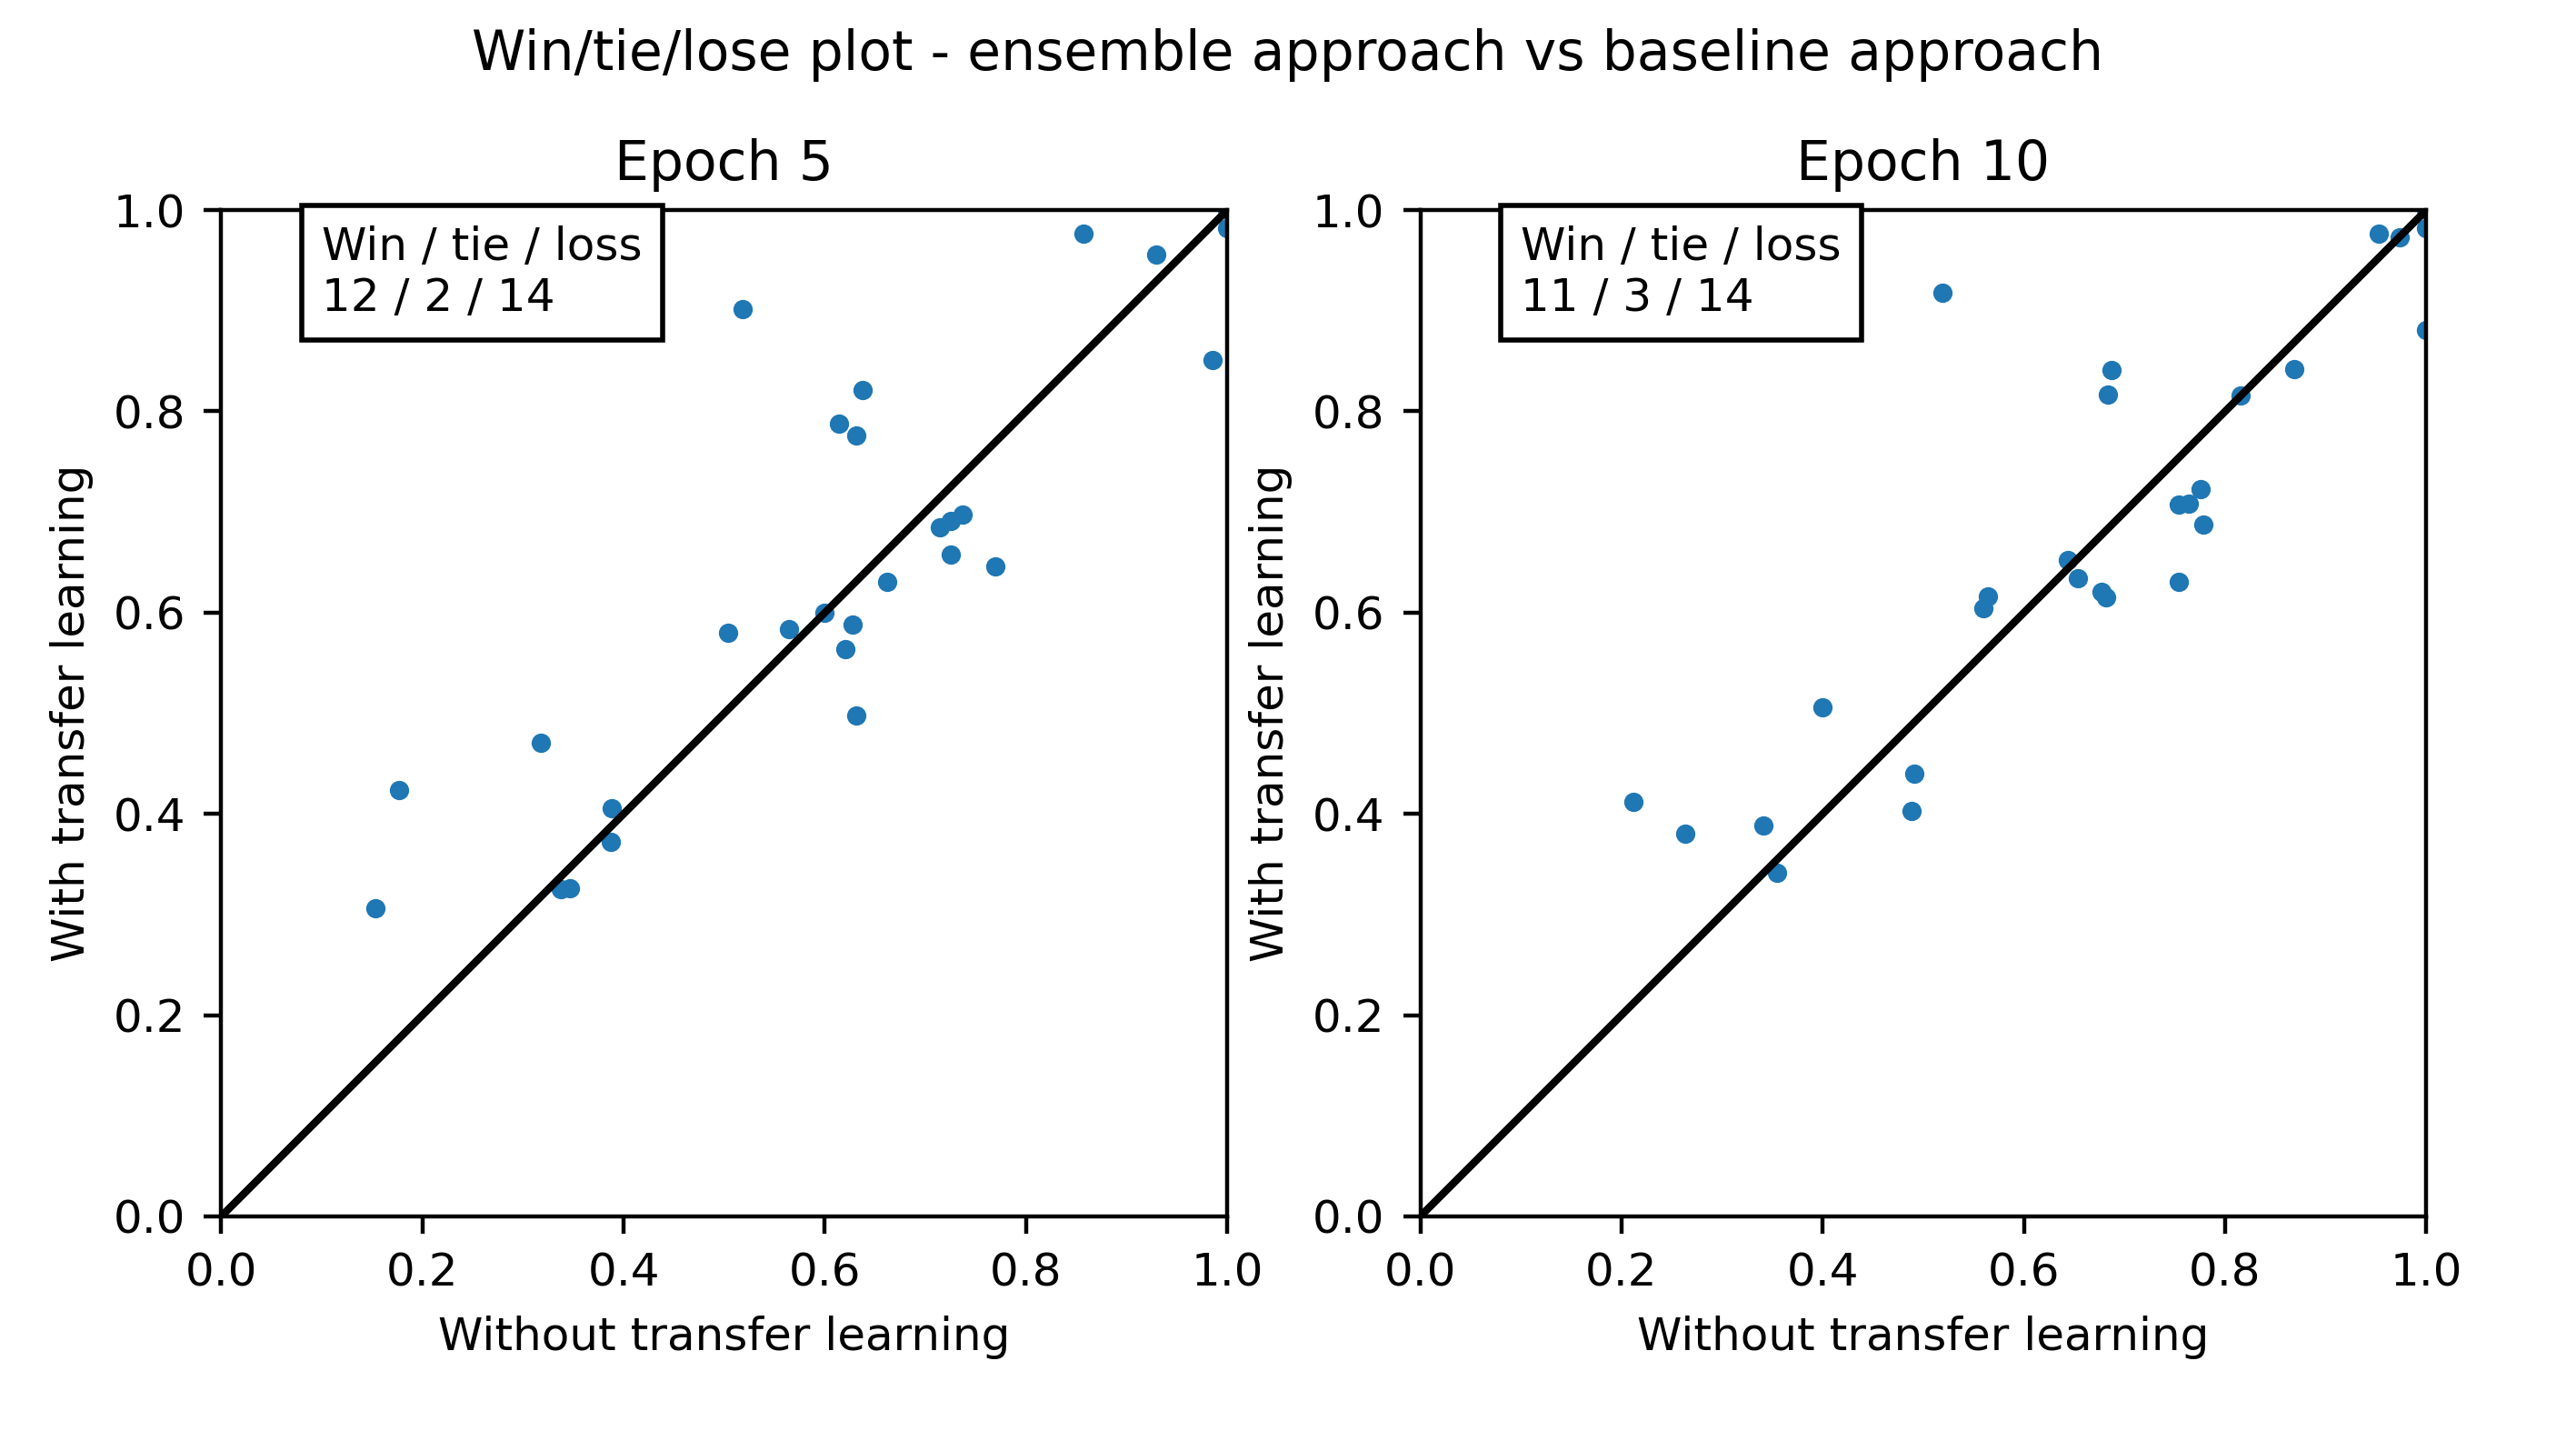
\includegraphics[width=17cm]{imgs/baseline_vs_ensemble/win_tie_lose_epoch.png}
\caption{Win-tie-loss diagram  for\textit{ baseline } and\textit{ ensemble }approach. Dot above the diagonal line means that the run (corresponding to training on a particular dataset)  achieved better results with the \textit{ensemble} approach.}
\label{fig:win_tie_loss_baseline_vs_ensemble}
\end{figure}
\FloatBarrier

Other than the differences in qualitative results, the computation time and sizes of the classifiers differ in both approaches.
For the baseline approach, the model is smaller, and it takes less time to pre-train a single model with a large amount of data than to pre-train a few small separate models with smaller data. Therefore, the time needed to pre-train the network in the \textit{baseline} approach is longer than in the \textit{ensemble} approach.

Training the model used in the \textit{ensemble} approach comprises two steps. In the first step, each component, a single FCN model, is trained on a single dataset corresponding to each source dataset selected for the target dataset. Hence it is a single dataset and a single model. This could be parallelized, as the models and datasets and independent. The second step consists of training the model on the ensemble created from the pre-trained components on the target dataset. The resulting model is larger than the final classifier in the \textit{baseline} approach. Summing up, pre-training the ensemble components and training the network takes longer than in the \textit{baseline} approach. The training procedure in the baseline approach consists of training the source (single) model on the combined dataset and retraining it on the target dataset.
Figure \ref{fig:baseline_ensemble_traning_time} compares training time for both approaches. The training time shown on the plot is the sum needed for the pre-training and fine-tuning steps.
\FloatBarrier
\begin{figure}[h!t]
\centering
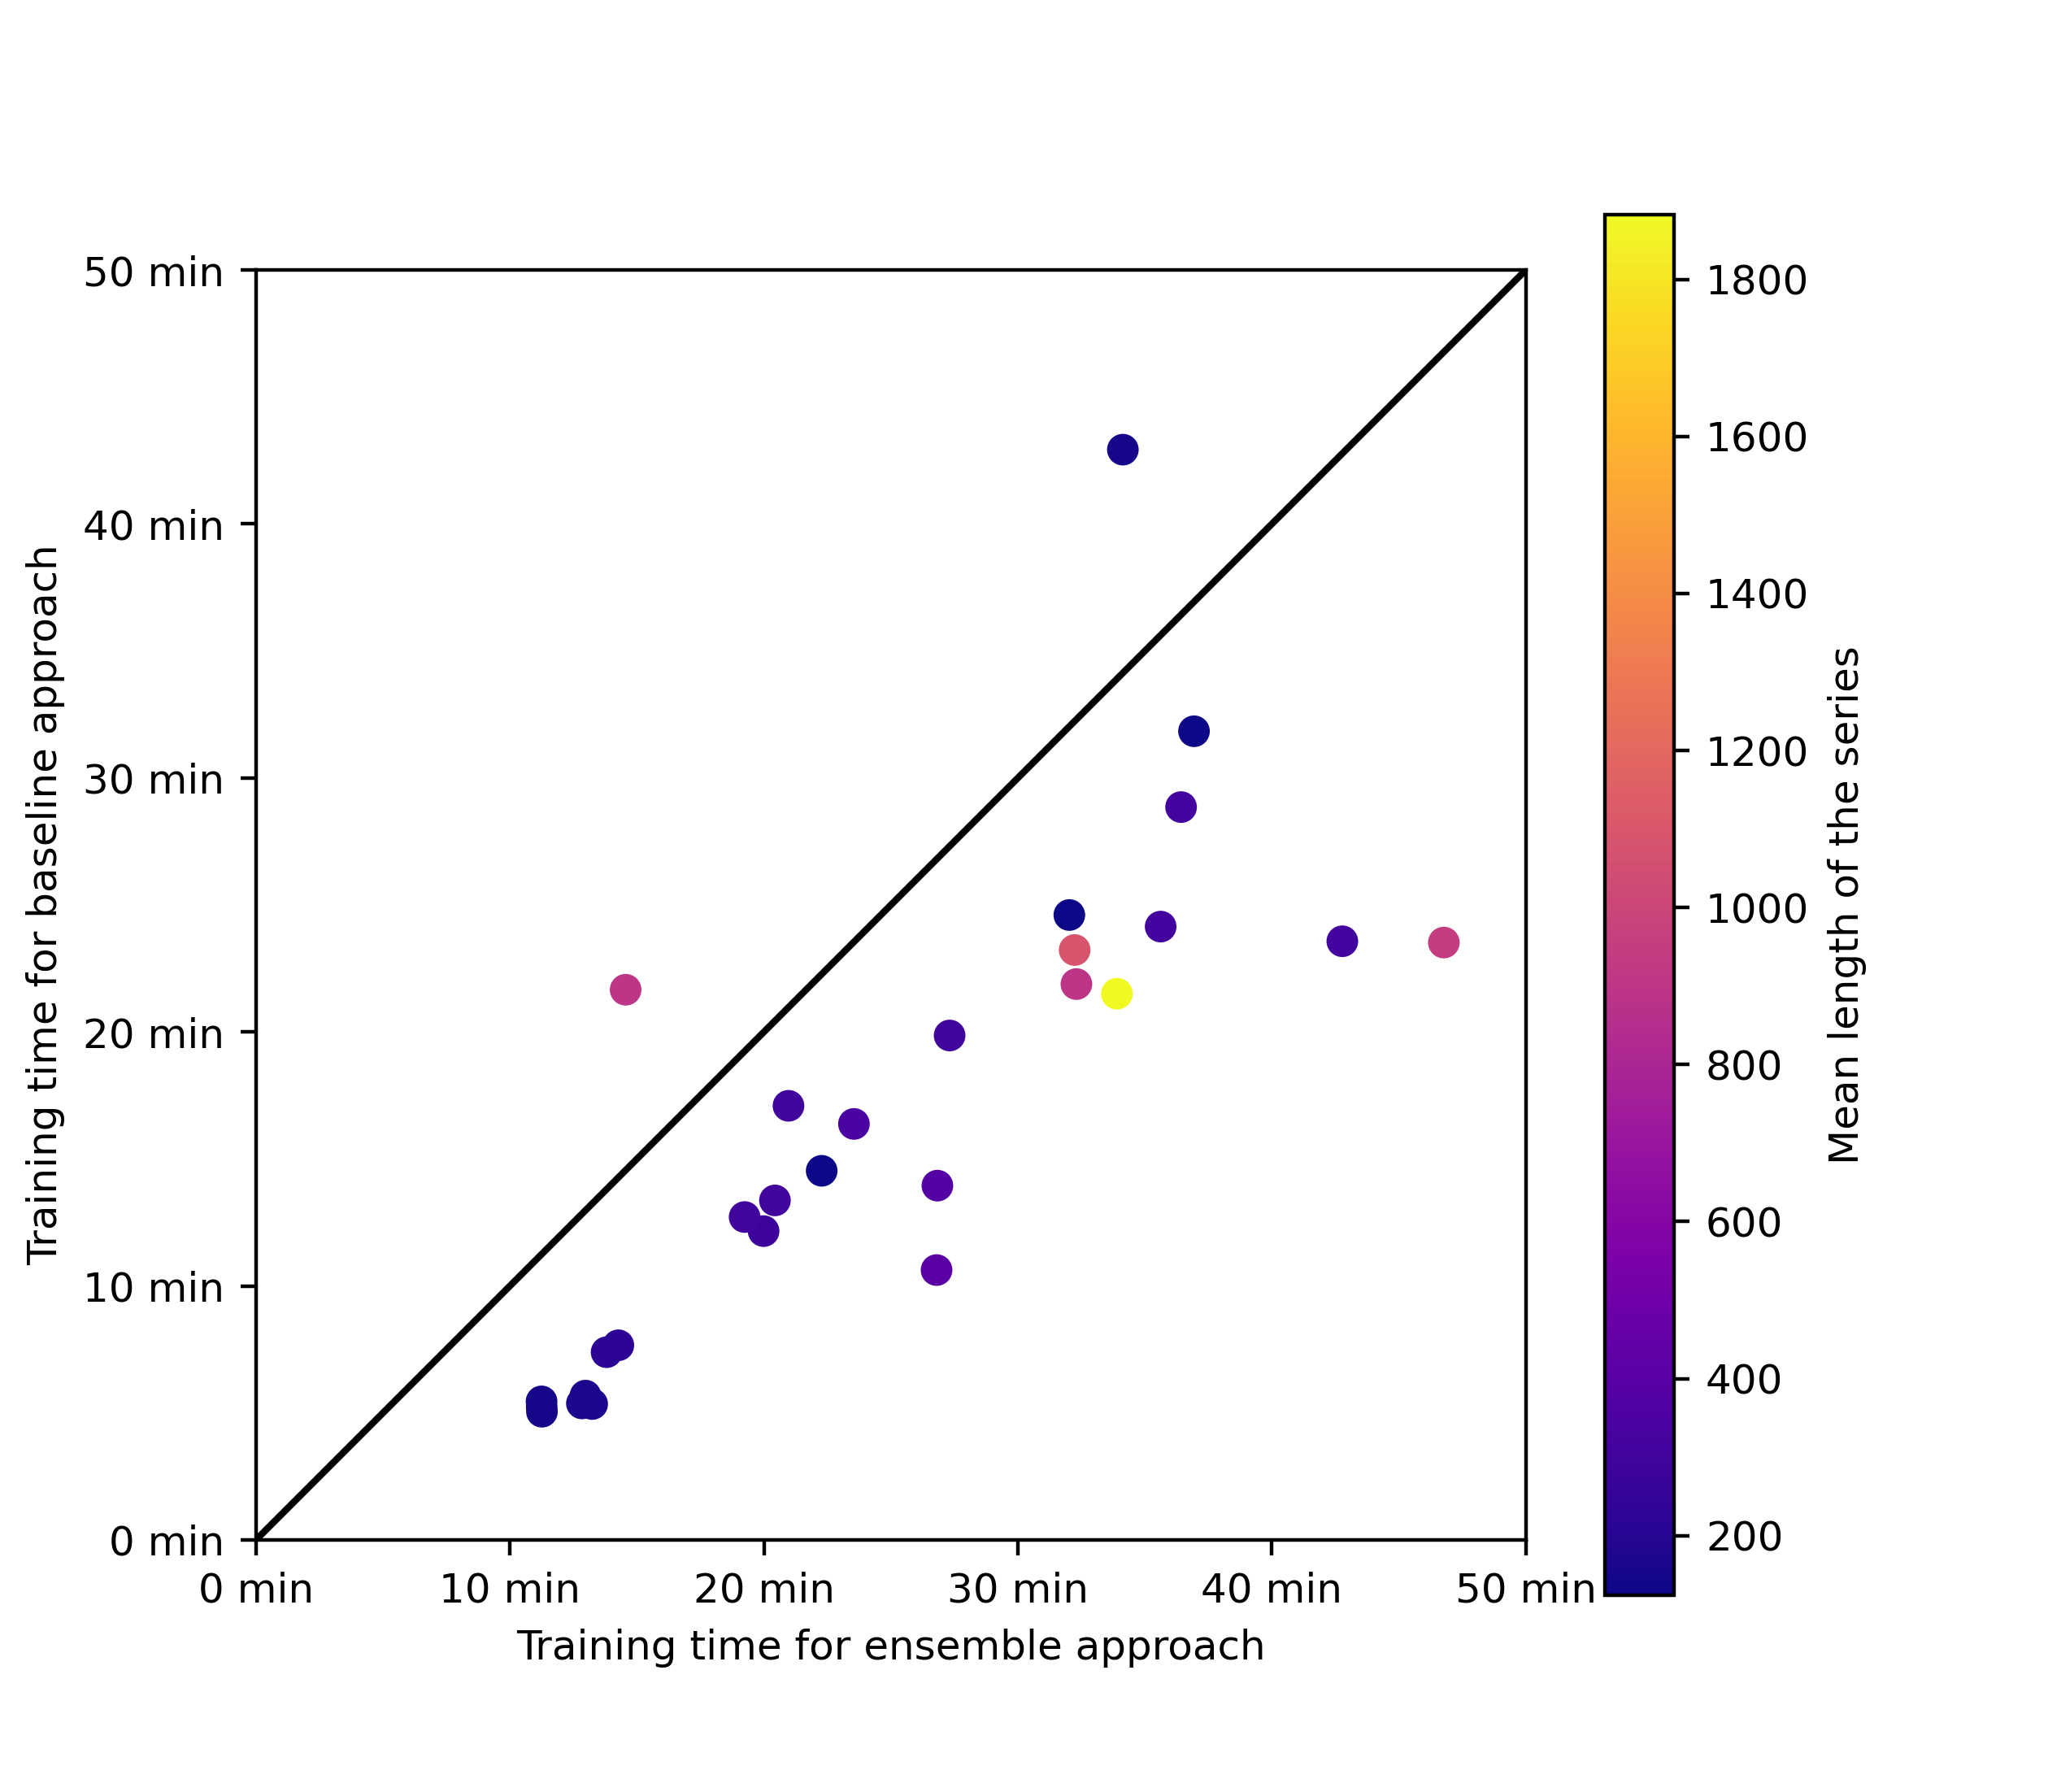
\includegraphics[width=17cm]{imgs/baseline_vs_ensemble/times_comparison.png}
\caption{The total time needed to train the source classifier/classifiers and the target classifier in \textit{baseline} and \textit{ensemble} methods. The color shows the total length of the series (source and target dataset).}
\label{fig:baseline_ensemble_traning_time}
\end{figure}
\FloatBarrier
It is worth mentioning that during the experiments conducted for the sake of this thesis, much time was saved by saving the components pre-trained for the \textit{ensemble}. If a component was trained once on a given source dataset, it was reused every time an ensemble model was created of it. It saved time during the experiments, but the time saved was not deducted from the time shown in Figure \ref{fig:baseline_ensemble_traning_time}.

When it comes to the size of the model, the model used for \textit{baseline} approach consisted of c.a. (depending on the number of classes) $266 000$ parameters, while the model used for \textit{ensemble} approach (created from $5$ components) consisted typically of $1 332 000$ parameters. The model weights used for \textit{baseline} occupied 3.22 MB after saving on disk (as a TensorFlow Checkpoint), and the model weights used for the ensemble approach (created from $5$ components) used 16.04 MB of disk memory.

\section{Evaluation os source datasets selection method}
As mentioned in \ref{section:selecting}, the datasets used for multi-source transfer learning were selected in two ways: randomly or based on the DBA similarity measure. This section contains a comparison of those two methods. The selecting method is independent of the model, thus it can be used for both \textit{ensemble} and \textit{baseline} approaches. Unfortunately, this evaluation is performed only using the \textit{ensemble} approach, given the time and computational limitations.

Figure \ref{fig:random_vs_dba} shows the averaged results using random selection and selection based on the DBA similarity measure.

As we see, selecting the datasets based on the similarity measure led to slight improvement.
\FloatBarrier
\begin{figure}[h!t]
\centering
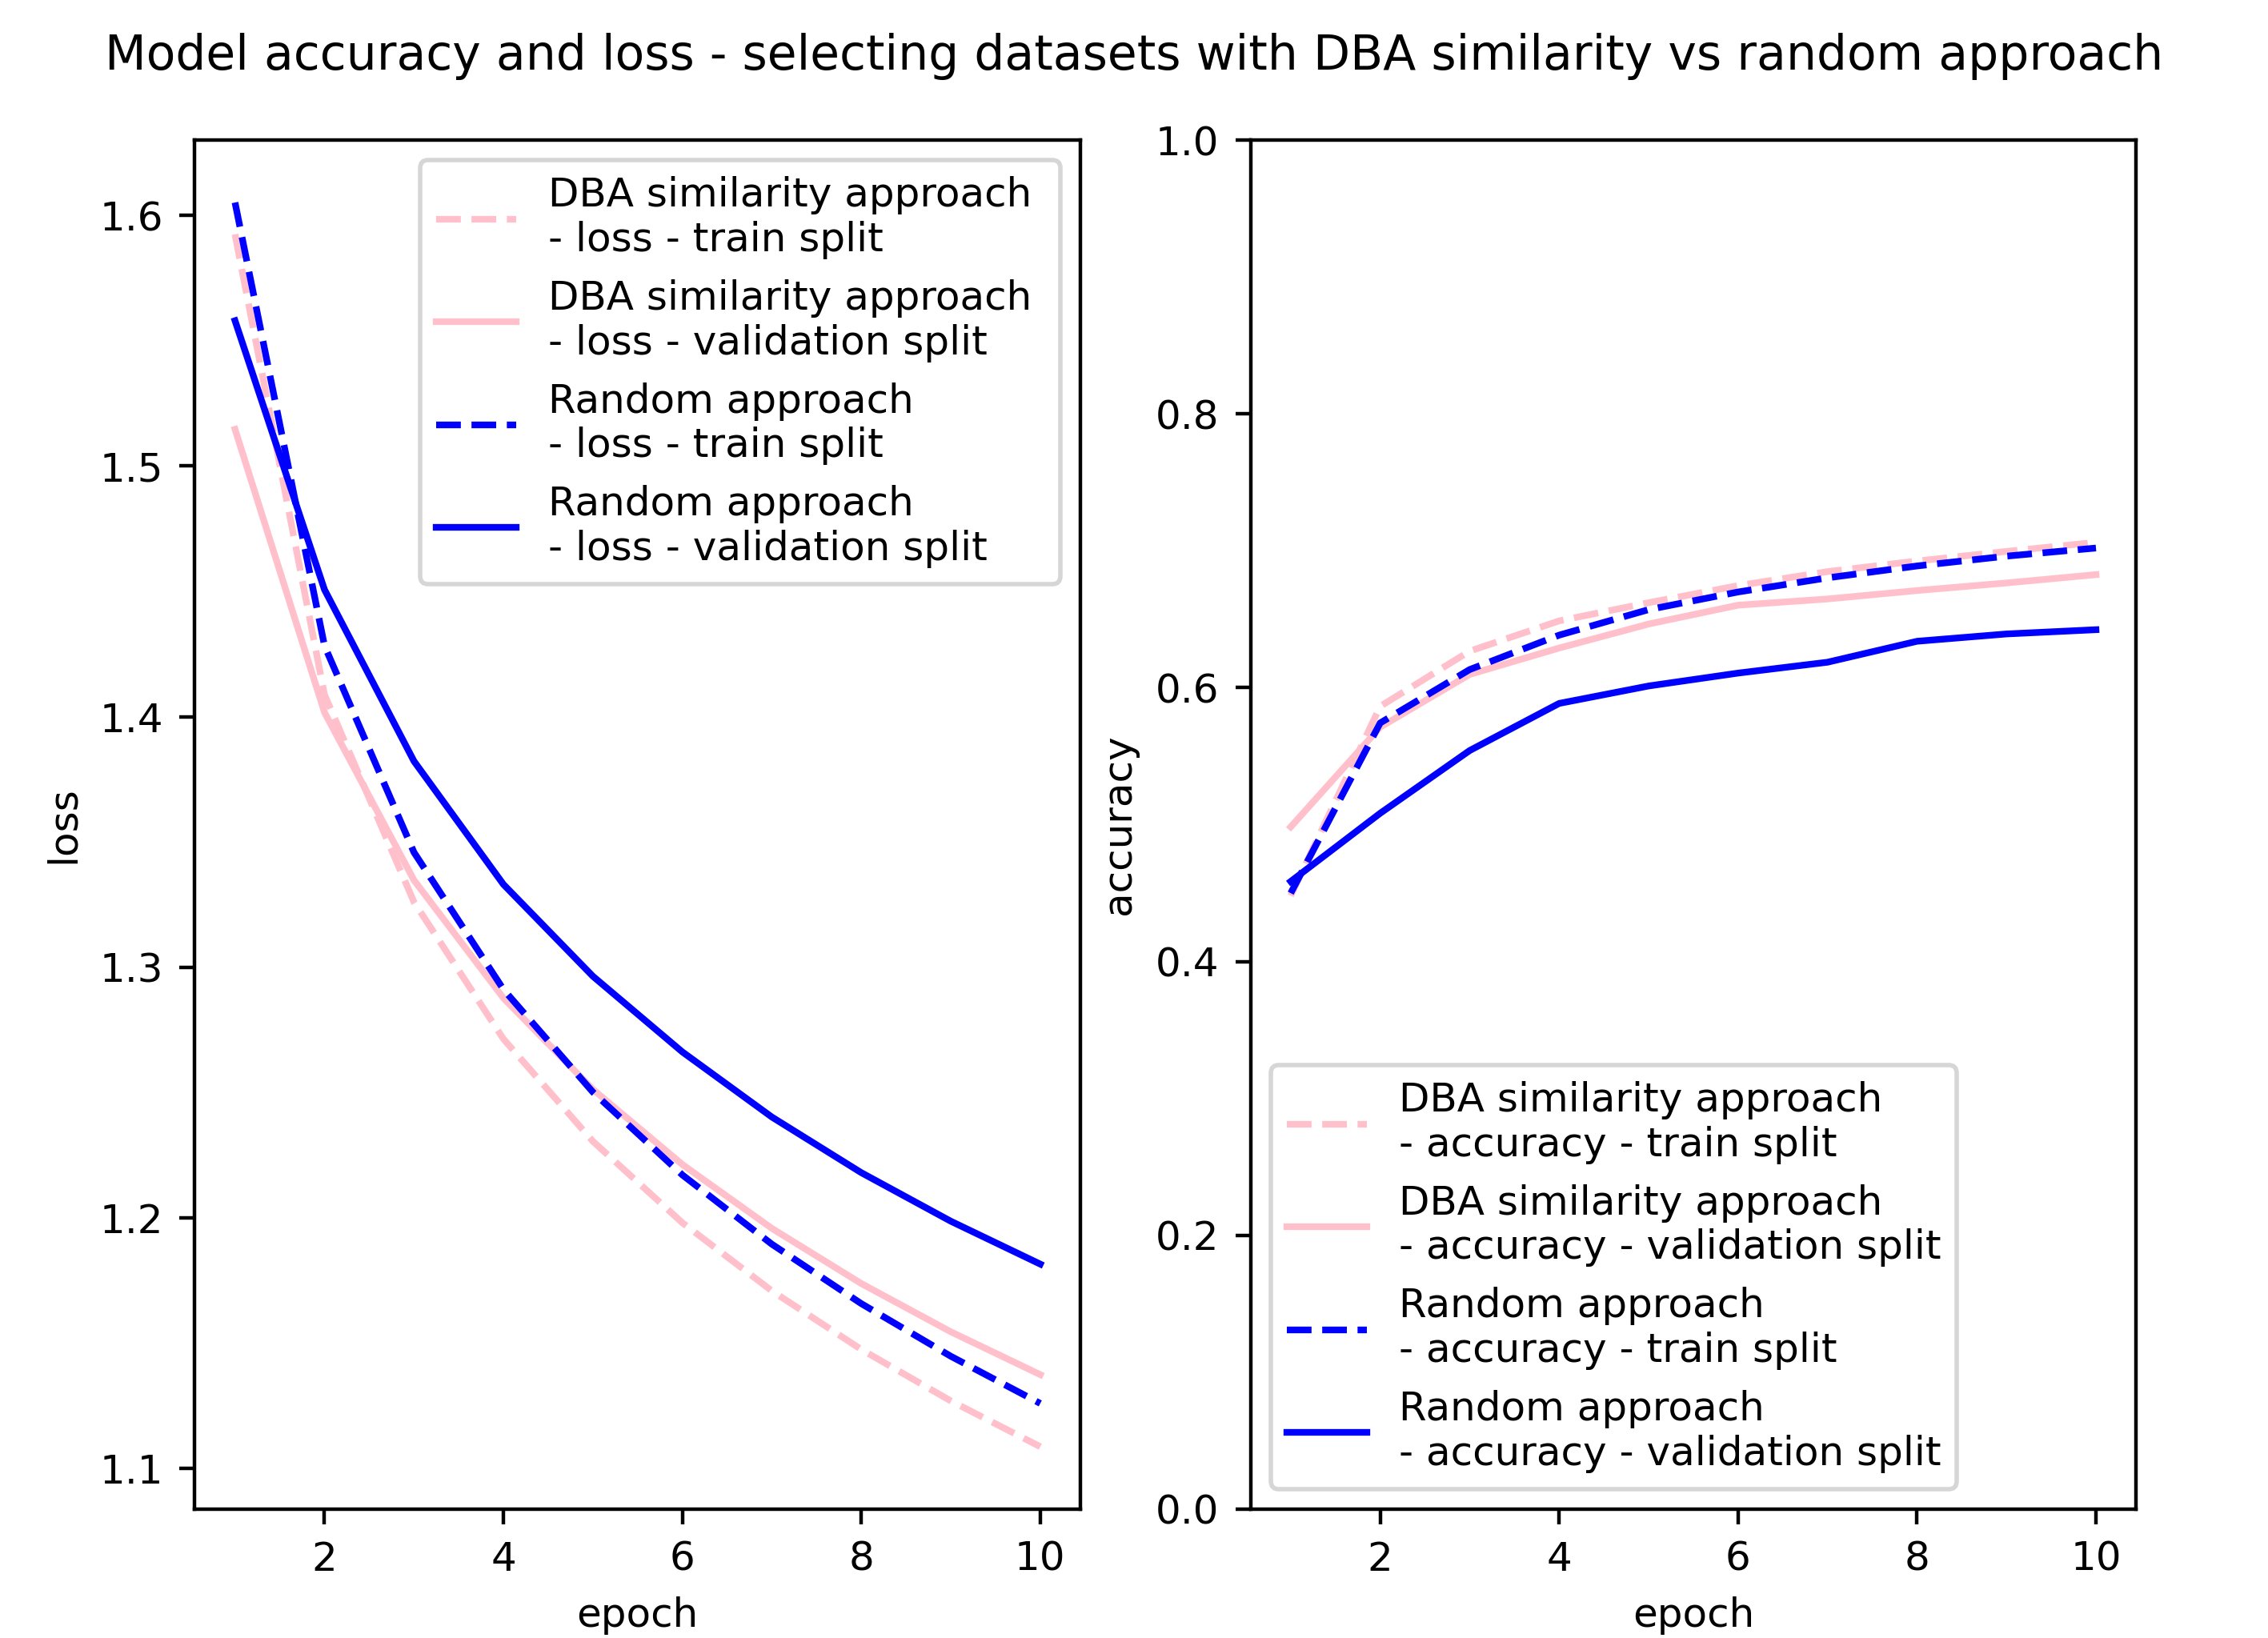
\includegraphics[width=17cm]{imgs/dba_vs_random/loss_acc.png}
\caption{Averaged accuracy and loss per each epoch for the ensemble approach when selecting the source datasets randomly and using the DBA similarity approach.}
\label{fig:random_vs_dba}
\end{figure}
\FloatBarrier
The win-tie-loss diagram also indicates an advantage of the DBA selection approach (Figure \ref{fig:random_vs_dba_win_tie_loss}

\FloatBarrier
\begin{figure}[h!t]
\centering
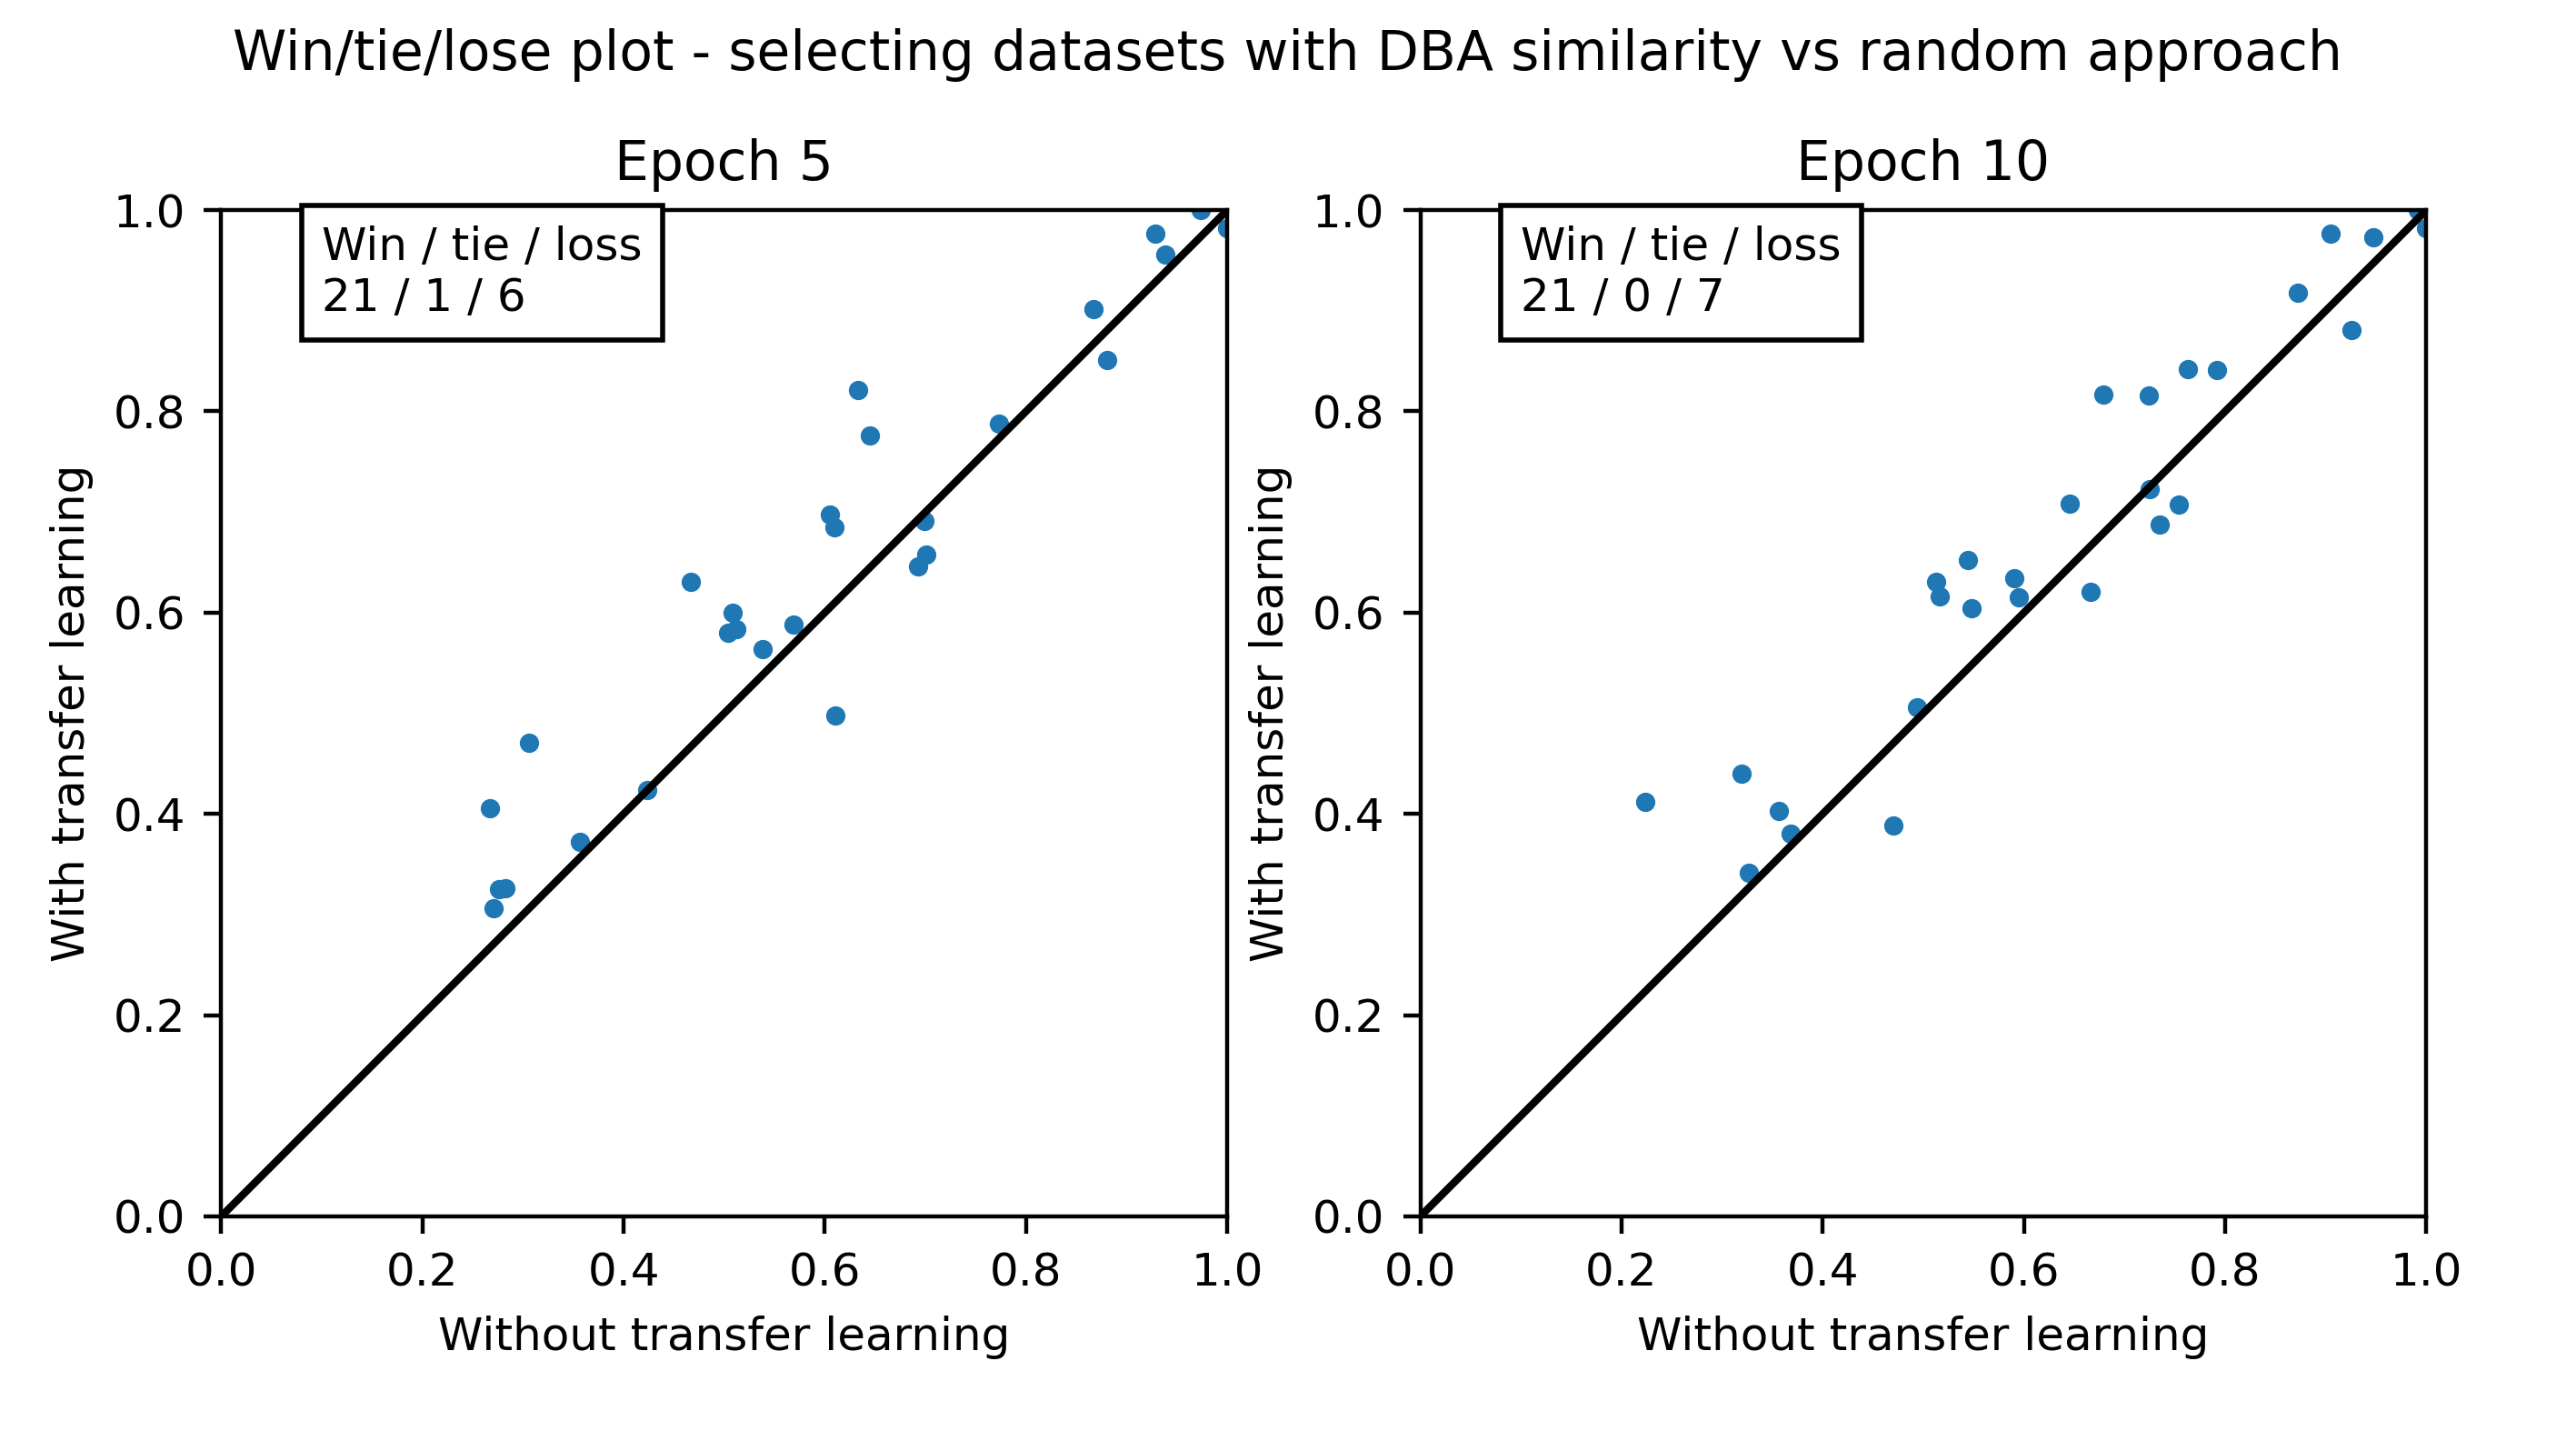
\includegraphics[width=17cm]{imgs/dba_vs_random/win_tie_lose_epoch.png}
\caption{Win-tie-loss diagram comparing selecting the source datasets randomly vs with the DBA similarity approach.}
\label{fig:random_vs_dba_win_tie_loss}
\end{figure}
\FloatBarrier
There is still room to improve the similarity measure. In order to understand the improvements in accuracy when using similarity score, the correlation between the target classifier accuracy and the dba similarity has been examined. The scatterplot is shown on plot \ref{fig:acc_vs_dba_sim}.
\FloatBarrier
\begin{figure}[h!t]
\centering
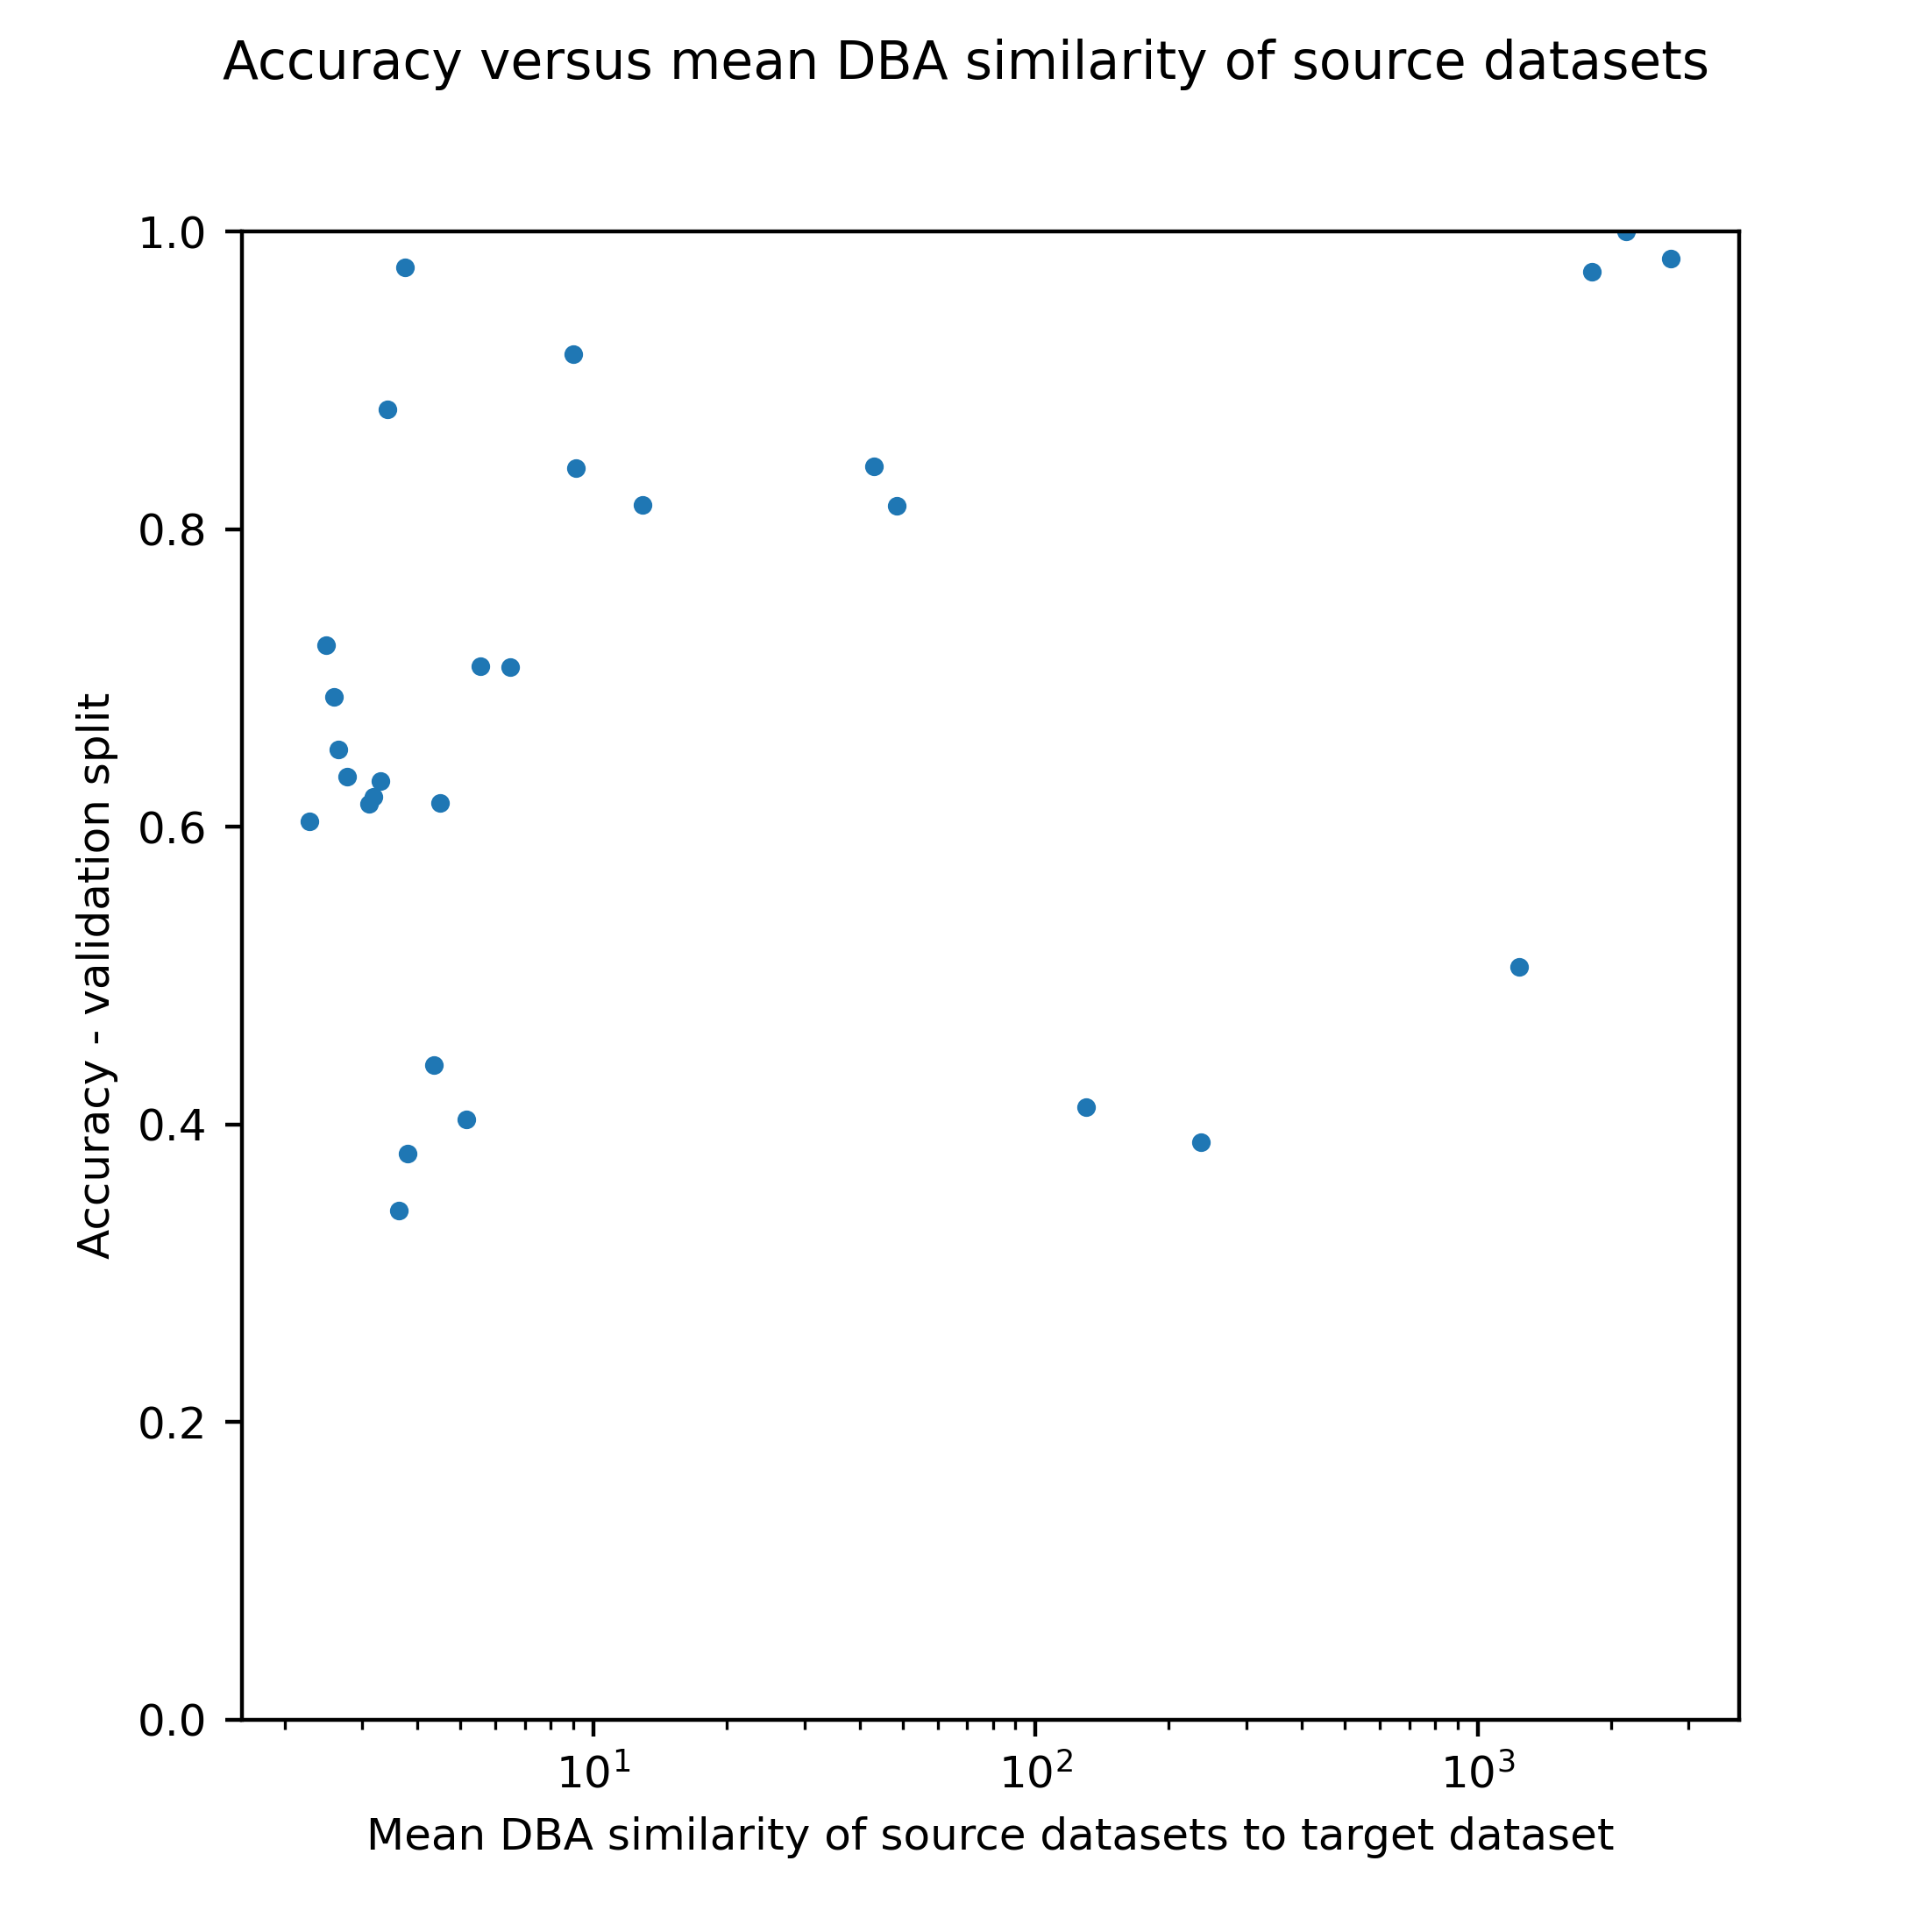
\includegraphics[width=17cm]{imgs/ensemble/accuracy_vs_mean_dba_sim.png}
\caption{}
\label{fig:acc_vs_dba_sim}
\end{figure}
\FloatBarrier
\section{Influence of accuracy of the components used in the ensemble on the target classifiers' accuracy}
This short section checks the hypothesis that the better the model we use in \textit{ensemble} approach, the better the final results on the target classifier. As we see on the plot \ref{fig:acc_source_vs_acc_target}, which shows the mean accuracy of components (measured on each source dataset, using test split) versus the accuracy of the target classifier (measured on the test split of target dataset). The correlation between the two statistics is very moderate (0.15).
\FloatBarrier
\begin{figure}[h!t]
\centering
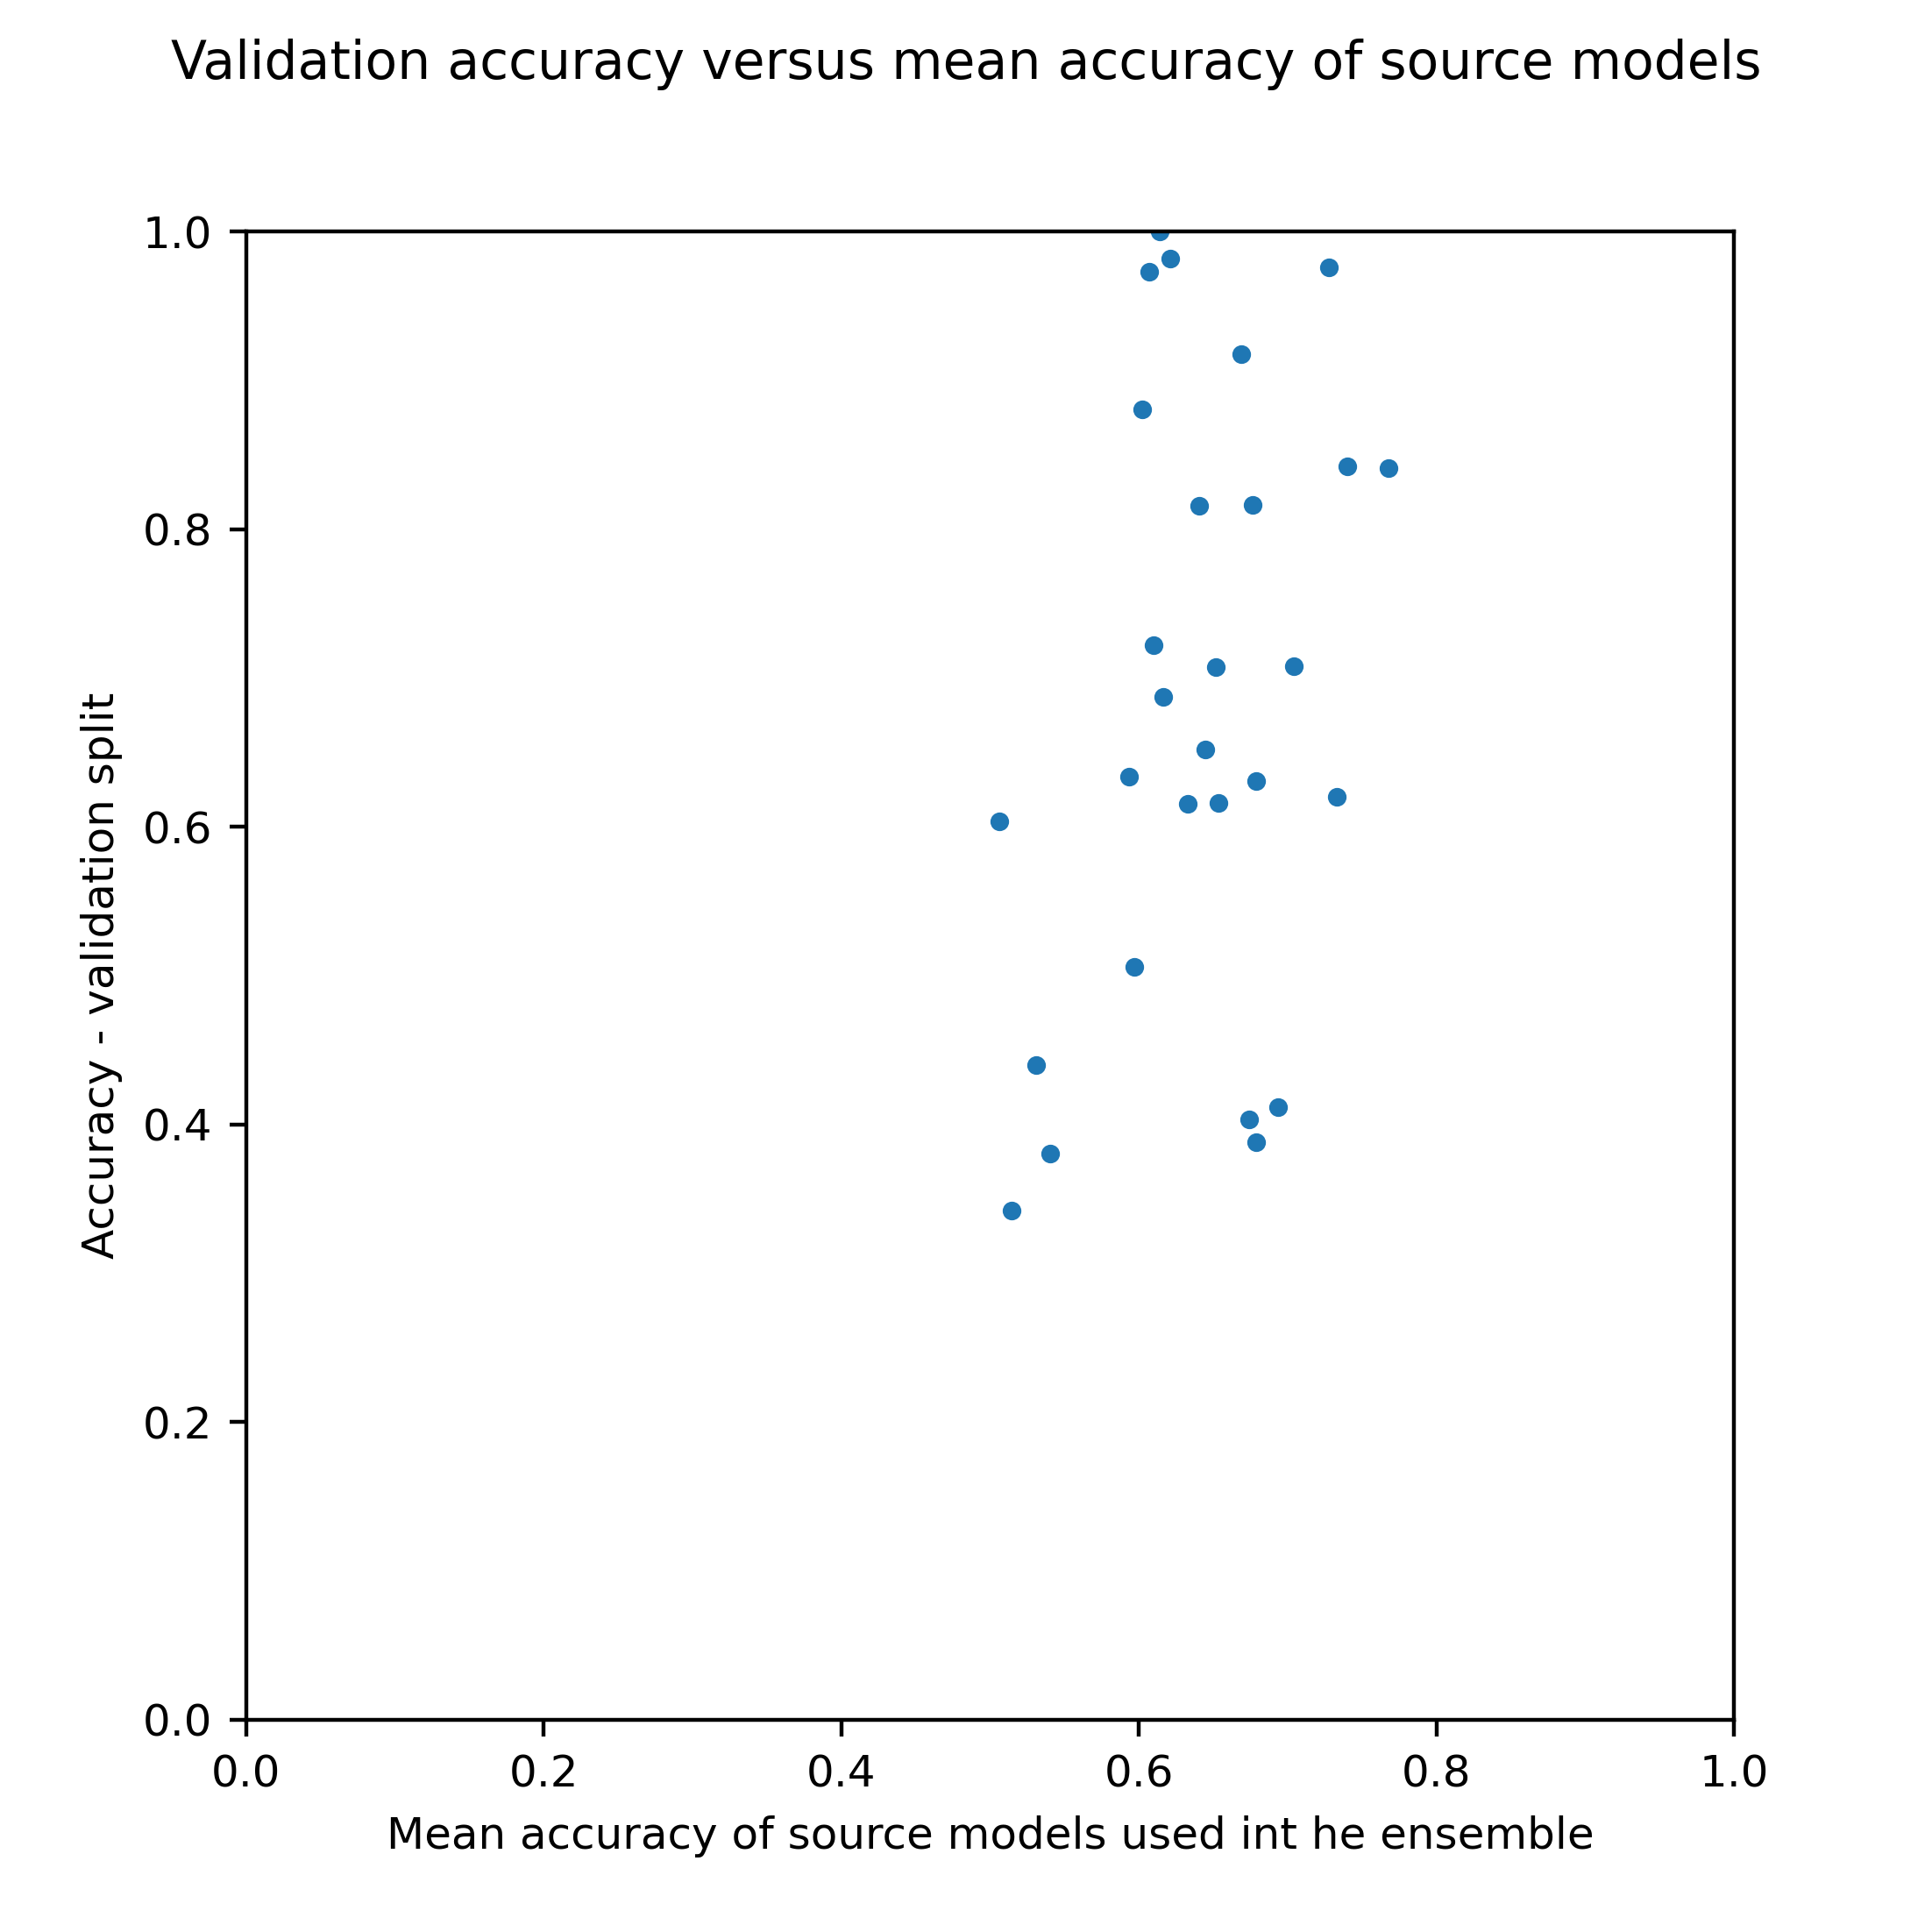
\includegraphics[width=17cm]{imgs/ensemble/source_acc_vs_val.png}
\caption{The weak influence of the accuracy of classifiers used in the \textit{ensemble} method on the target classifier.}
\label{fig:acc_source_vs_acc_target}
\end{figure}
\FloatBarrier
\section{Number of datasets used in multi-source transfer learning}
We used $5$ source datasets for the previous experiments, both for the \textit{ensemble} and \textit{baseline} approach. However, the number of experiments is arbitrary. Similarly, as in the previous sections, we compared \textit{ensemble} and \textit{baseline} approaches to models trained without transfer learning. We compared the accuracy and loss for models pre-trained with $3$, $5$, and $8$ source datasets.

We found that all configurations give good results, while using $5$ datasets gives the best results. Figure \ref{fig:ensemble_3_5_8} shows the averaged accuracy and loss plot. For this comparison, we used the ensemble approach and the DBA similarity measure.

\FloatBarrier
\begin{figure}[h!t]
\centering
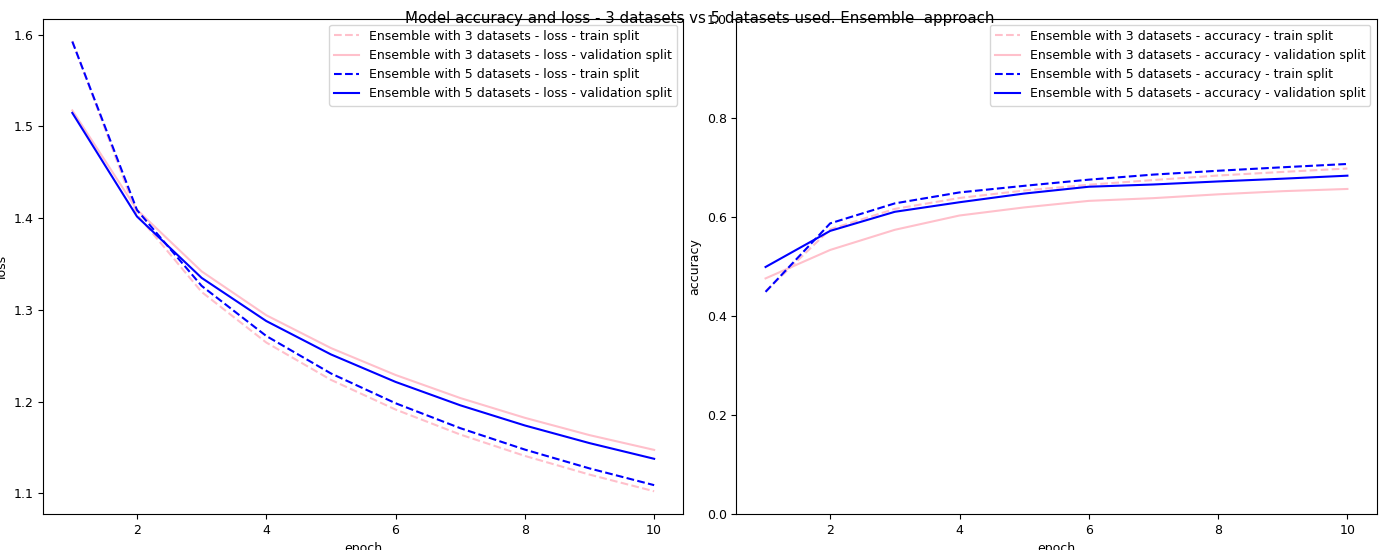
\includegraphics[width=17cm]{imgs/ensemble_dba_3_vs_5/loss_acc.png}
\caption{Accuracy and loss on each epoch, averaged over several target datasets}
\label{fig:ensemble_3_5_8}
\end{figure}
\FloatBarrier


Figures \ref{fig:ensemble_3_5_win_tie_loss} and
\ref{fig:ensemble_5_8_win_tie_loss} also presents the win-tie-loss diagram comparing the same experiment with 3 and 5 datasets, and with 5 and 8 datasets.


\FloatBarrier
\begin{figure}[h!t]
\centering
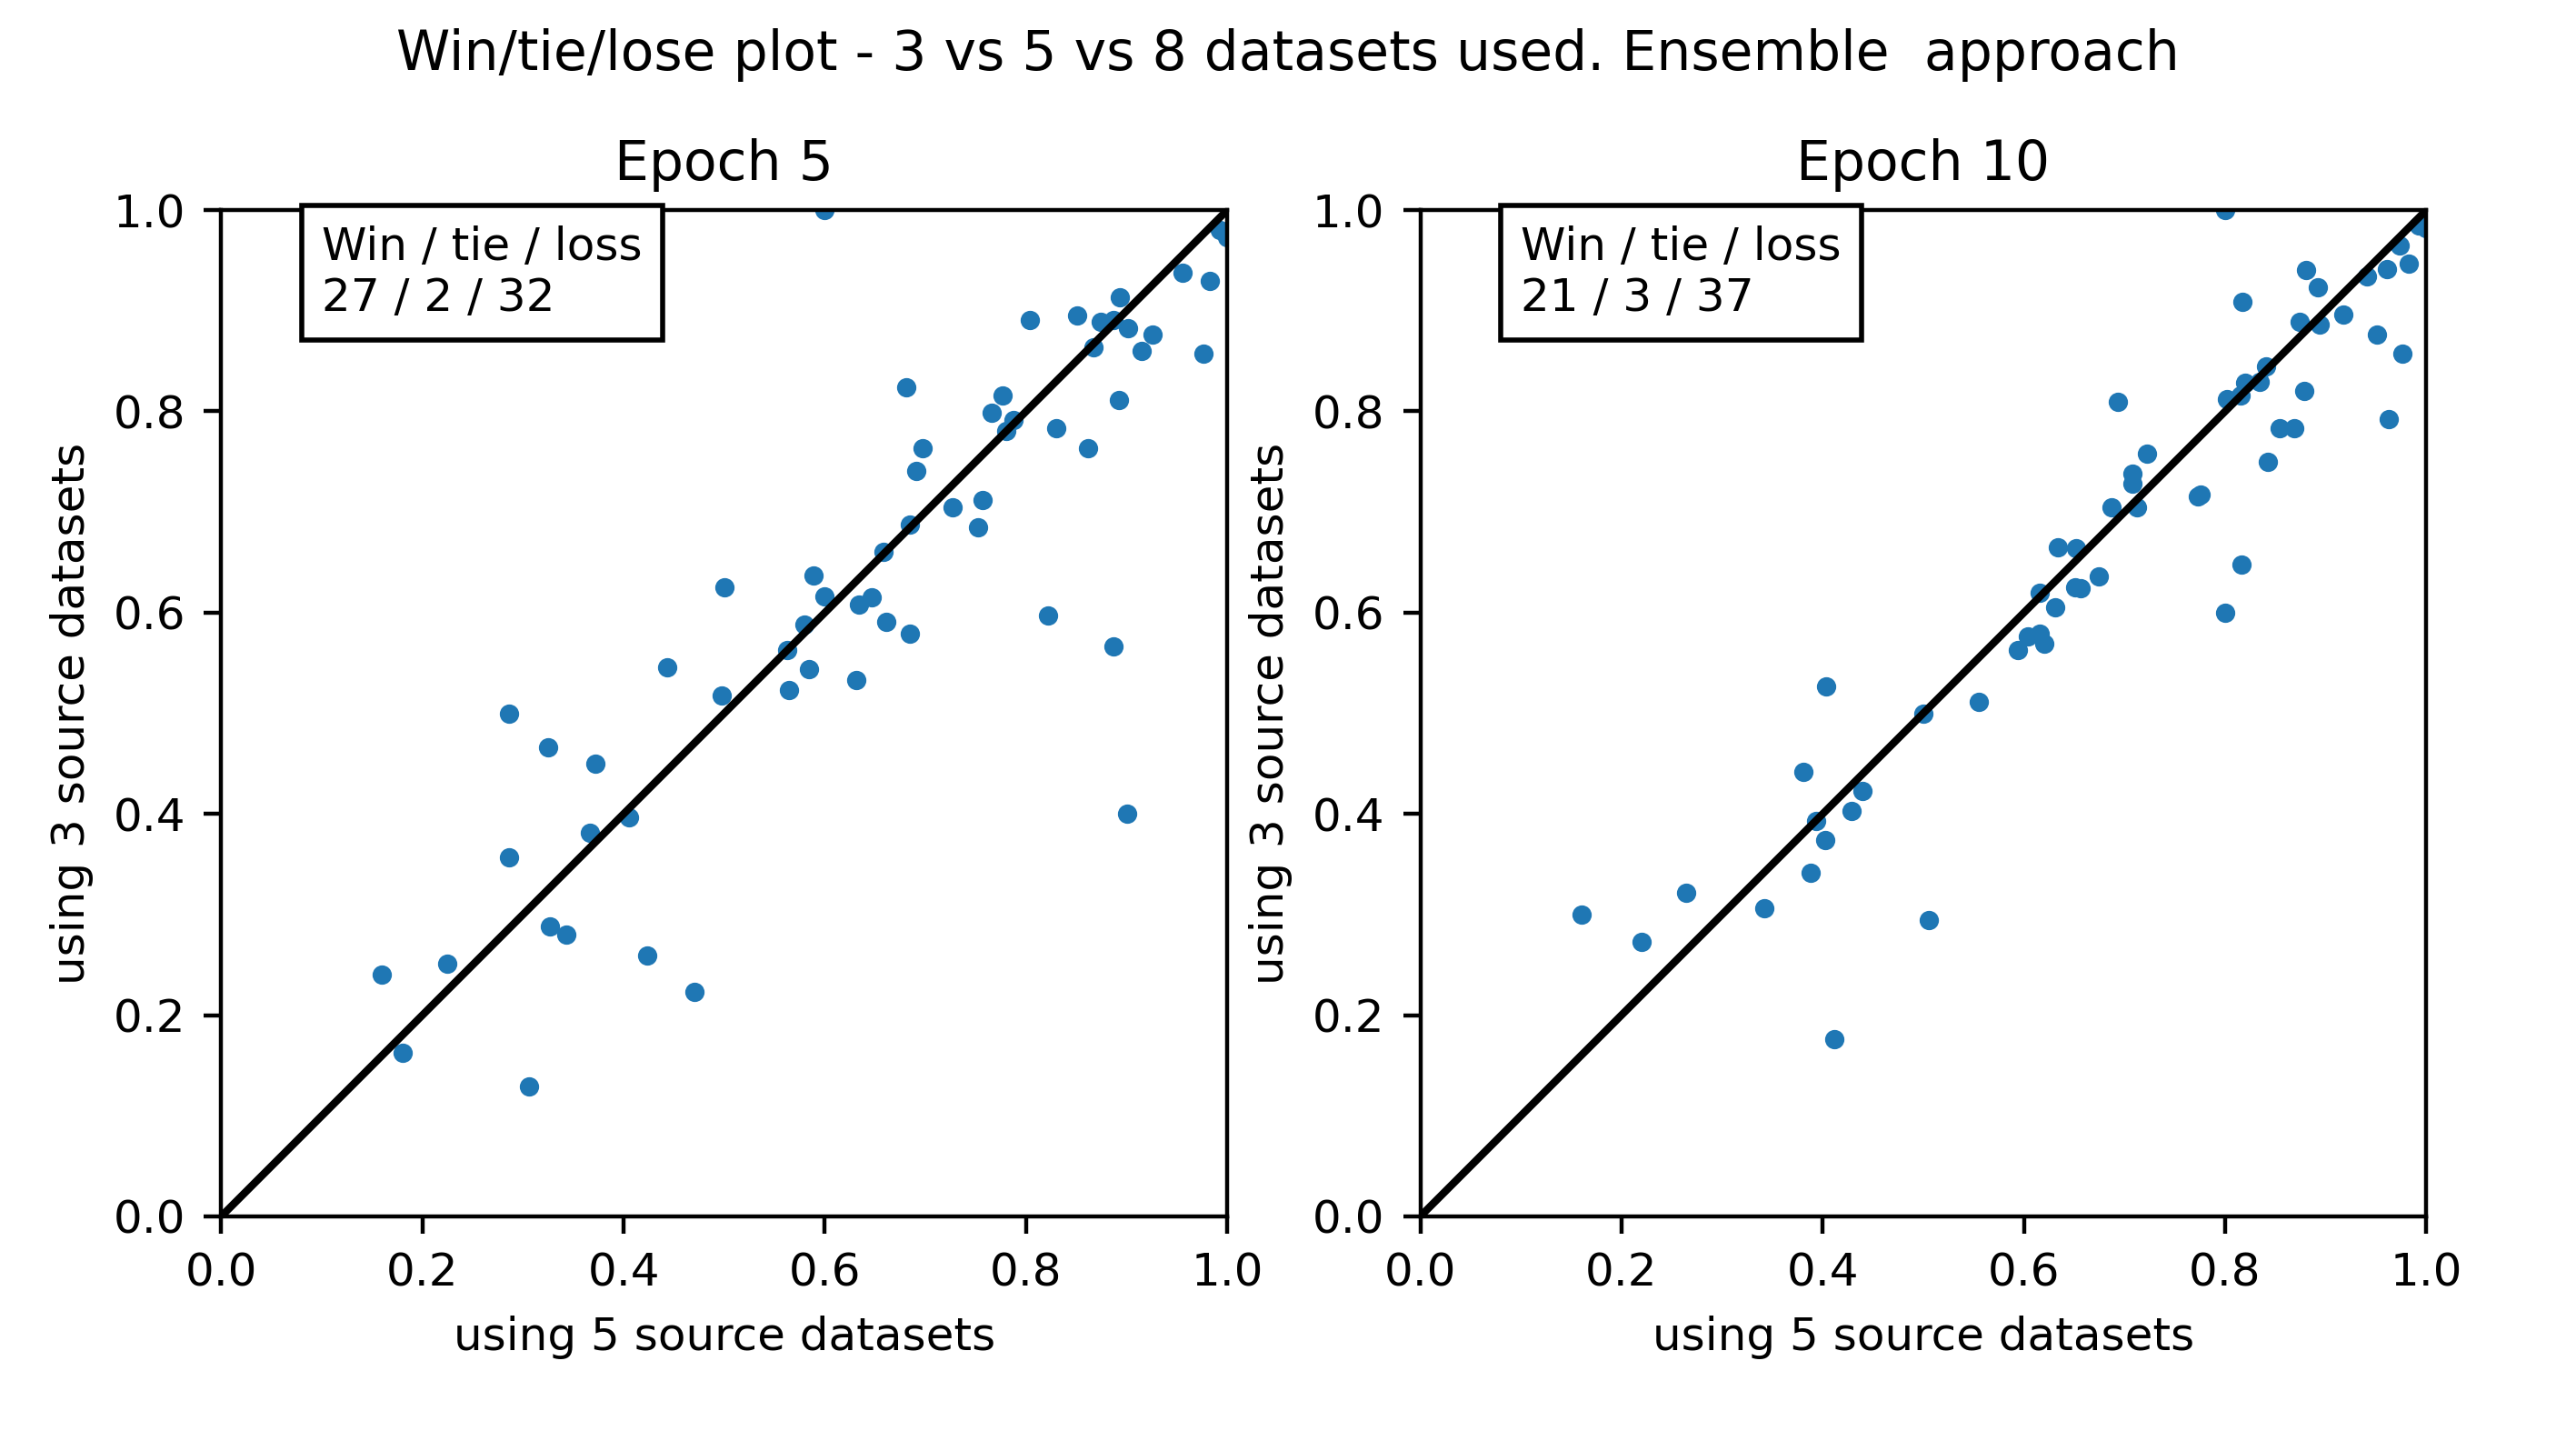
\includegraphics[width=17cm]{imgs/ensemble_dba_3_vs_5/win_tie_lose_epoch.png}
\caption{Win-tie-loss diagram comparing the ensemble approach with 3 and 5 datasets (DBA similarity measure is used for choosing the source datasets}
\label{fig:ensemble_3_5_win_tie_loss}
\end{figure}
\FloatBarrier
\begin{figure}[h!t]
\centering
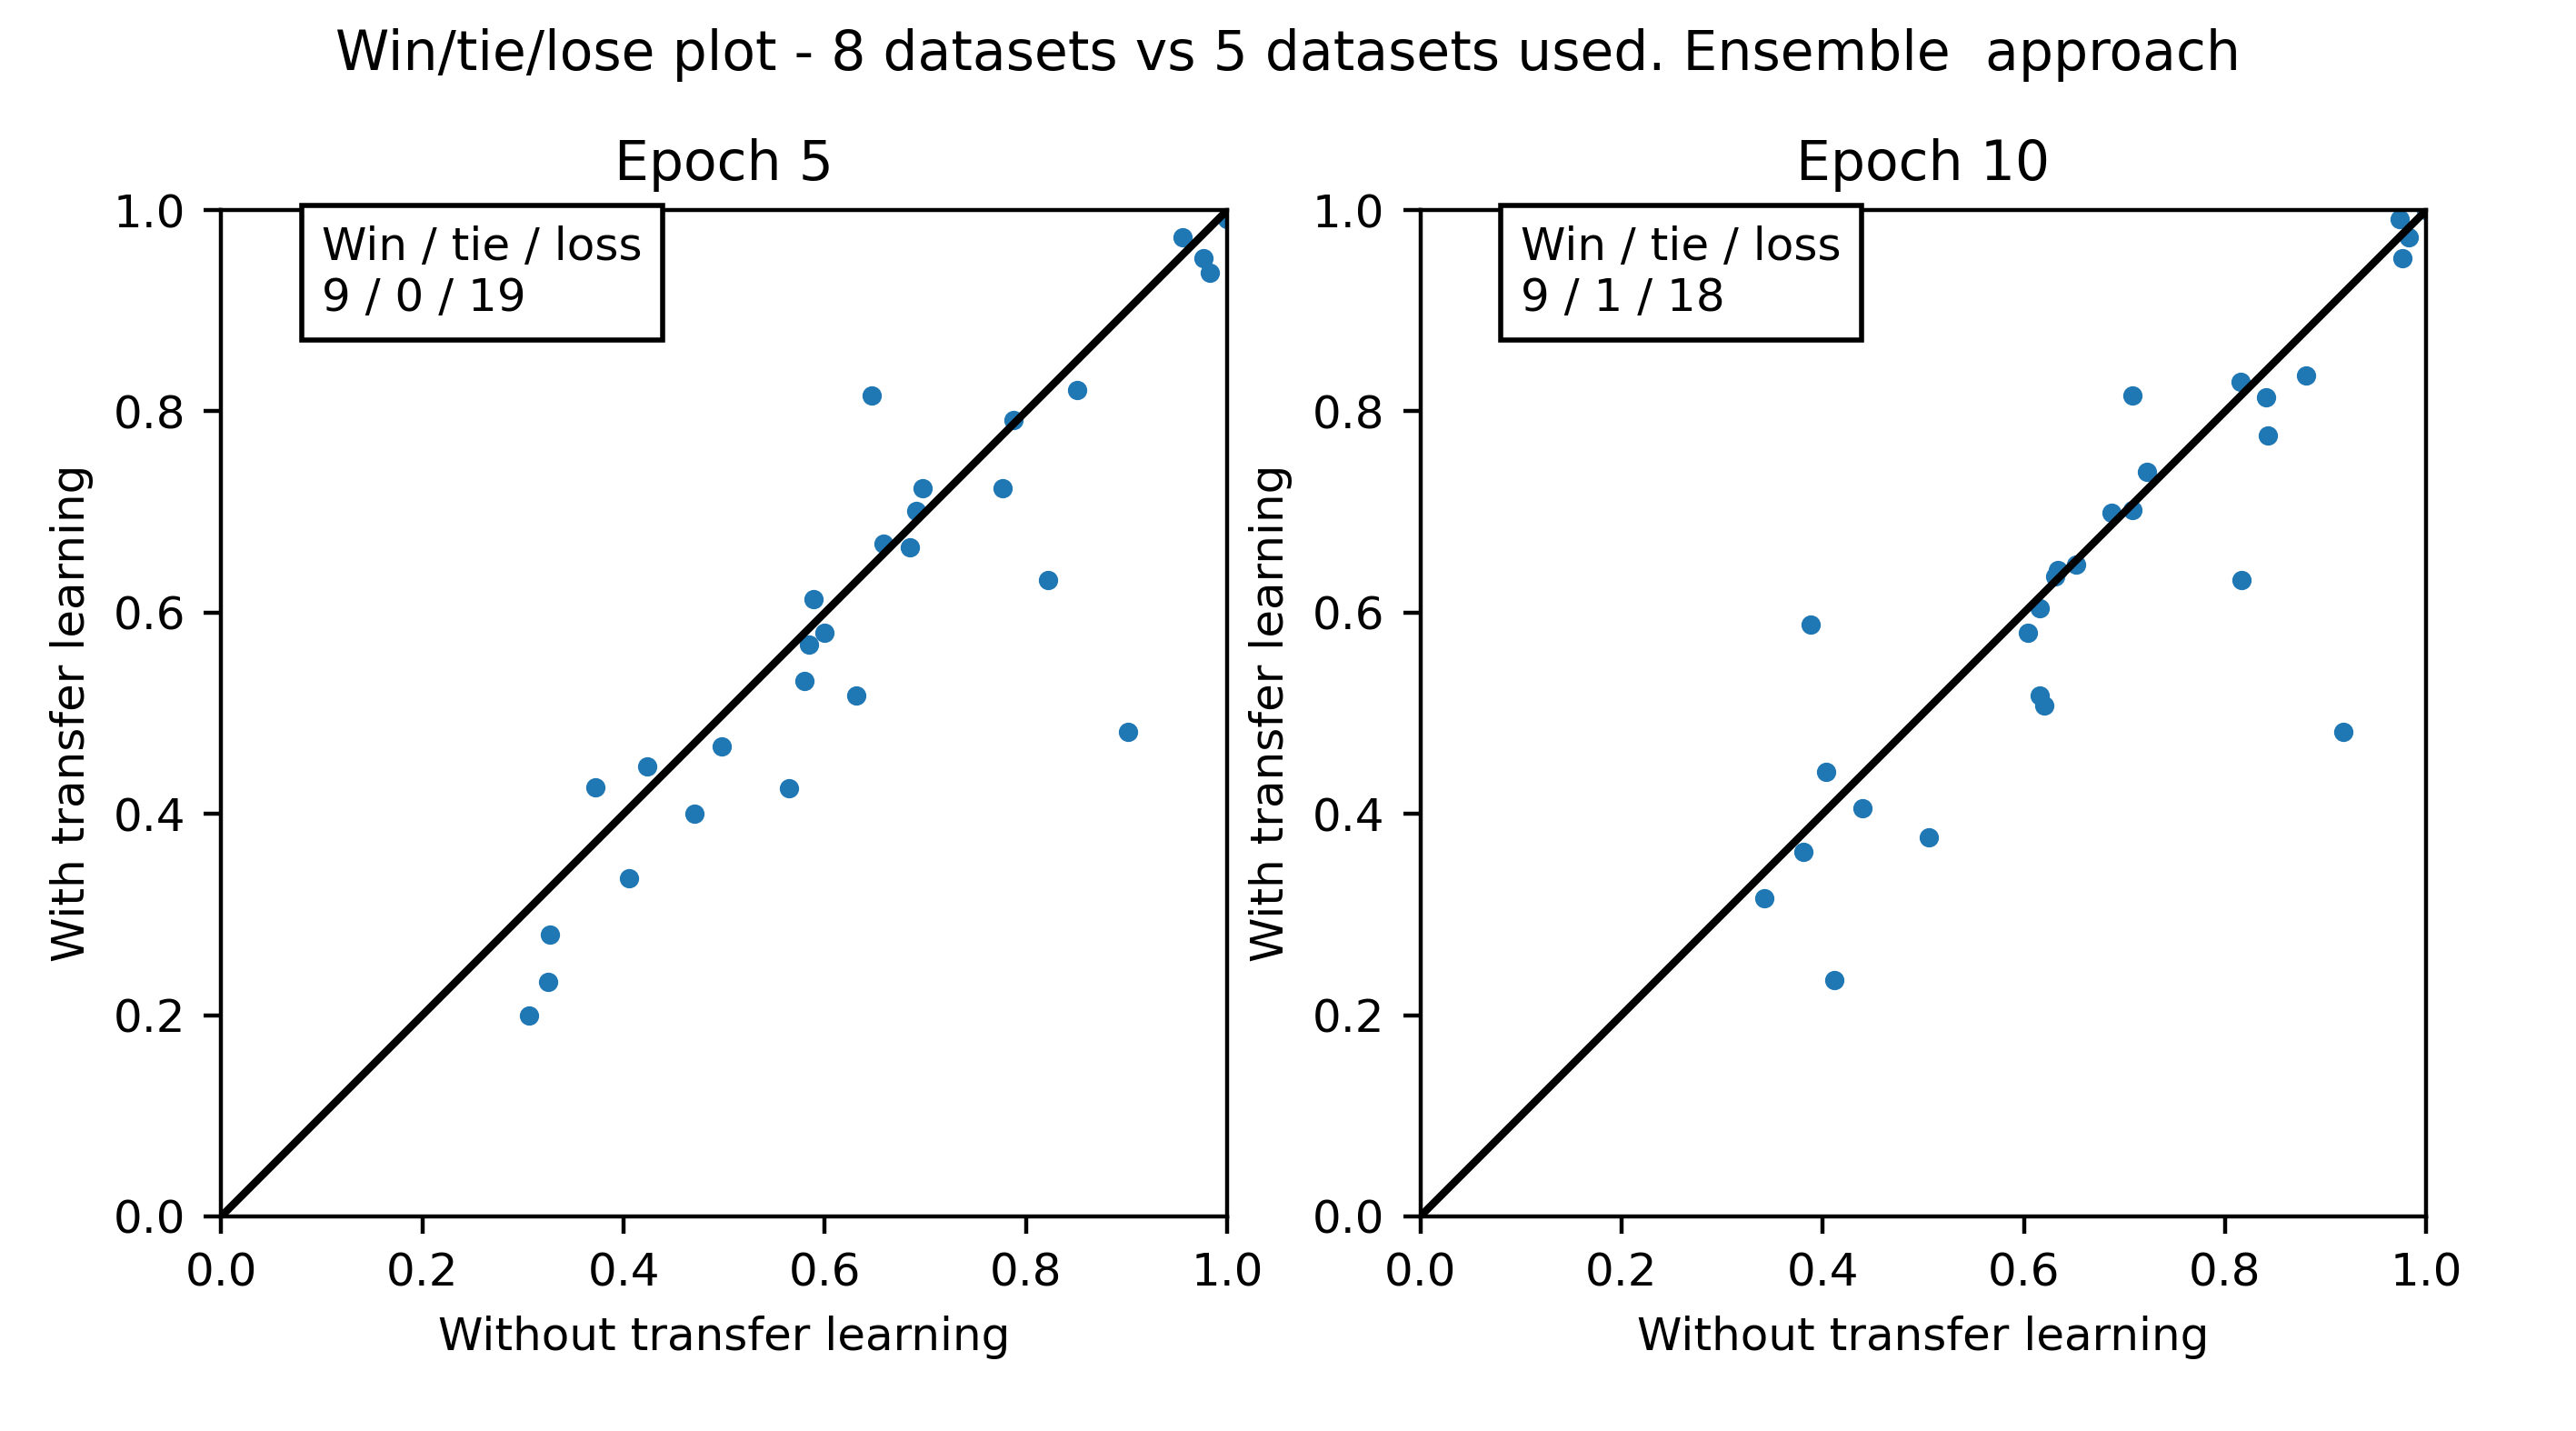
\includegraphics[width=17cm]{imgs/ensemble_dba_5_vs_8/win_tie_lose_epoch.png}
\caption{Win-tie-loss diagram comparing the ensemble approach with 5 and 8 datasets (DBA similarity measure is used for choosing the source datasets}
\label{fig:ensemble_5_8_win_tie_loss}
\end{figure}
\FloatBarrier
\chapter{Conclusions}

In this thesis, we extended the research on transfer learning in time series classification. We proposed two approaches to multi-source transfer learning: the \textit{baseline} and \textit{ensemble} approach, the second inspired by the success of ensemble classifiers in the time series classification domain. The \textit{baseline} approach can be summarized as pre-training a neural network on a concatenated dataset consisting of multiple datasets and then using the weights from the first layers to initialize the final classifier. In the \textit{ensemble} approach, we train several models, each on a different source dataset. Then we construct an ensemble of those models initialized with the weights obtained from pre-training. We have proven that for both approaches, multi-source transfer learning increased the accuracy of the classifiers. The usage of transfer learning also mitigated overfitting, which is very common for small datasets present in the time series classification domain. Furthermore, a detailed comparative analysis of the two approaches was conducted.

The \textit{ensemble} approach proved to be better in terms of performance results. However, the size of the ensemble model may be a limitation, especially with larger networks, bigger datasets, or environments with limited memory. Furthermore, the \textit{ensemble} approach is slightly slower, as we train multiple classifiers, and the resulting model is bigger. However, training the ensemble's component models can be parallelized, the components can be reused, and time can be saved.


We also considered two methods of selecting the datasets for pre-training the source classifiers. The method based on the DBA similarity measure has proven to be slightly advantageous compared to choosing the datasets randomly or by trial and error. We believe that this method may be improved by enhancing the similarity measure.

We also experimented with the number of source datasets. Experiments were conducted using $3$, $5$, and $8$, using the \textit{ensemble} approach. All of those settings resulted in decent results, and using $5$ datasets was averagely more effective than using $3$ or $8$ datasets.

\section{Further works}
As an extension to the work done for this thesis, we may consider an extension to the source dataset selection algorithm. We may consider measuring the similarity of shapelets, as those are the critical attributes learned by convolutional layers.

Also, architectures other than Fully Convolutional Networks could be used in the future. Both \textit{ ensemble }and\textit{ baseline} approaches generally apply to deep neural networks. As we focused on the transfer learning aspect and the computational resources were limited, we tested only the Fully Convolutional Network architecture. It may be worth considering performing the same analysis but using a fixed input size network, long short-term memory network, or residual networks.

The study may also be extended to testing datasets outside of the UCR time series archive or testing transfer learning between different categories in the UCR archive, which wasn't planned in the scope of this thesis due to computational limitations.

The number of datasets used for both \textit{ensemble} or \textit{baseline} approaches can be further studied. We can consider numbers other than $3$, $5$, and $8$ (e.g.,~using all datasets available in the UCR archive). The effort could be combined with improving the similarity measure in order to develop a method to obtain the optimal number of datasets given the similarity measure, e.g.,~with stepwise selection of datasets similar, as in stepwise feature selection.





% ------------------------------- BIBLIOGRAPHY ---------------------------
% LEXICOGRAPHICAL ORDER BY AUTHORS' LAST NAMES
% FOR AMBITIOUS ONES - USE BIBTEX
\
\bibliographystyle{plain} % We choose the "plain" reference style
\bibliography{refs} % Entries are in the refs.bib file


\pagenumbering{gobble}
\thispagestyle{empty}



% ----------------------- LIST OF SYMBOLS AND ABBREVIATIONS ------------------
%\chapter*{List of symbols and abbreviations}
%
%\begin{tabular}{cl}
%nzw. & nadzwyczajny \\
%* & star operator \\
%$\widetilde{}$ & tilde
%\end{tabular}
%\\
%If you don't need it, delete it.
%\thispagestyle{empty}
%
%
%% ----------------------------  LIST OF FIGURES --------------------------------
%\listoffigures
%\thispagestyle{empty}
%If you don't need it, delete it.
%
%
%% -----------------------------  LIST OF TABLES --------------------------------
%\renewcommand{\listtablename}{Spis tabel}
%\listoftables
%\thispagestyle{empty}
%If you don't need it, delete it.
%
%% -----------------------------  LIST OF APPENDICES ---------------------------
%\chapter*{List of appendices}
%\begin{enumerate}
%\item Appendix 1
%\item Appendix 2
%\item In case of no appendices, delete this part.
%\end{enumerate}
%\thispagestyle{empty}


\end{document}
%
%\FloatBarrier
%
%\begin{figure}[h!t]
%\centering
%\includegraphics[width=17cm]{}
%\caption{}
%\label{fig:baseline_acc}
%\end{figure}
%\FloatBarrier
